% UPDATES:
%DIF LATEXDIFF DIFFERENCE FILE
%DIF DEL vStrCueCoding_v3.tex   Tue Jan 30 16:29:44 2018
%DIF ADD vStrCueCoding_v4.tex   Tue Mar  6 23:04:19 2018
% Version 1.2 - JG initial import of text and figures from Google Drive, with edits

\documentclass[11pt]{article}

% packages
\usepackage{natbib}
\usepackage{graphicx}
\usepackage[nolists]{endfloat}
\usepackage{times}
\usepackage{ifthen}
\usepackage{parskip}
\usepackage[font=sf,labelfont=bf]{caption}
\usepackage{xspace}
\usepackage[pdftex]{color}
\usepackage{pdfcolmk}
\usepackage{fixltx2e} % for \textsubscript
%\usepackage{epstopdf}

% line numbers
\usepackage[left]{lineno}

% variable margins
\usepackage[left=2.5cm,top=2.5cm,bottom=3.5cm,right=2.5cm]{geometry}

% this helps figure placement
\renewcommand{\textfraction}{0.0}
\renewcommand{\topfraction}{1}
\renewcommand{\bottomfraction}{1}


% convert tif to png for pdf
%\epstopdfDeclareGraphicsRule{.tif}{png}{.png}{convert #1 \OutputFile}
%\AppendGraphicsExtensions{.tif}

% spacing
\setlength{\parindent}{0in} 
\setlength{\parskip}{2\baselineskip}
\linespread{2}
\renewcommand{\baselinestretch}{1.66}\normalsize

% definitions
\newcommand{\bsf}[1]{\textbf{#1}}
\newcommand{\sem}{S.E.M.\@\xspace}
\newcommand{\degree}{$^o$\@\xspace}
\makeatletter
\setlength{\@fptop}{0pt}
\makeatother

% bib
\bibliographystyle{apa}
\let\cite=\citep
\let\citeN=\citet
\let\citeNP=\citealt
\renewcommand{\bibfont}{\footnotesize}
\setlength{\bibsep}{2pt}
%DIF PREAMBLE EXTENSION ADDED BY LATEXDIFF
%DIF UNDERLINE PREAMBLE %DIF PREAMBLE
\RequirePackage[normalem]{ulem} %DIF PREAMBLE
\RequirePackage{color}\definecolor{RED}{rgb}{1,0,0}\definecolor{BLUE}{rgb}{0,0,1} %DIF PREAMBLE
\providecommand{\DIFadd}[1]{{\protect\color{blue}\uwave{#1}}} %DIF PREAMBLE
\providecommand{\DIFdel}[1]{{\protect\color{red}\sout{#1}}}                      %DIF PREAMBLE
%DIF SAFE PREAMBLE %DIF PREAMBLE
\providecommand{\DIFaddbegin}{} %DIF PREAMBLE
\providecommand{\DIFaddend}{} %DIF PREAMBLE
\providecommand{\DIFdelbegin}{} %DIF PREAMBLE
\providecommand{\DIFdelend}{} %DIF PREAMBLE
%DIF FLOATSAFE PREAMBLE %DIF PREAMBLE
\providecommand{\DIFaddFL}[1]{\DIFadd{#1}} %DIF PREAMBLE
\providecommand{\DIFdelFL}[1]{\DIFdel{#1}} %DIF PREAMBLE
\providecommand{\DIFaddbeginFL}{} %DIF PREAMBLE
\providecommand{\DIFaddendFL}{} %DIF PREAMBLE
\providecommand{\DIFdelbeginFL}{} %DIF PREAMBLE
\providecommand{\DIFdelendFL}{} %DIF PREAMBLE
\newcommand{\DIFscaledelfig}{0.5}
%DIF HIGHLIGHTGRAPHICS PREAMBLE %DIF PREAMBLE
\RequirePackage{settobox} %DIF PREAMBLE
\RequirePackage{letltxmacro} %DIF PREAMBLE
\newsavebox{\DIFdelgraphicsbox} %DIF PREAMBLE
\newlength{\DIFdelgraphicswidth} %DIF PREAMBLE
\newlength{\DIFdelgraphicsheight} %DIF PREAMBLE
% store original definition of \includegraphics %DIF PREAMBLE
\LetLtxMacro{\DIFOincludegraphics}{\includegraphics} %DIF PREAMBLE
\newcommand{\DIFaddincludegraphics}[2][]{{\color{blue}\fbox{\DIFOincludegraphics[#1]{#2}}}} %DIF PREAMBLE
\newcommand{\DIFdelincludegraphics}[2][]{% %DIF PREAMBLE
\sbox{\DIFdelgraphicsbox}{\DIFOincludegraphics[#1]{#2}}% %DIF PREAMBLE
\settoboxwidth{\DIFdelgraphicswidth}{\DIFdelgraphicsbox} %DIF PREAMBLE
\settoboxtotalheight{\DIFdelgraphicsheight}{\DIFdelgraphicsbox} %DIF PREAMBLE
\scalebox{\DIFscaledelfig}{% %DIF PREAMBLE
\parbox[b]{\DIFdelgraphicswidth}{\usebox{\DIFdelgraphicsbox}\\[-\baselineskip] \rule{\DIFdelgraphicswidth}{0em}}\llap{\resizebox{\DIFdelgraphicswidth}{\DIFdelgraphicsheight}{% %DIF PREAMBLE
\setlength{\unitlength}{\DIFdelgraphicswidth}% %DIF PREAMBLE
\begin{picture}(1,1)% %DIF PREAMBLE
\thicklines\linethickness{2pt} %DIF PREAMBLE
{\color[rgb]{1,0,0}\put(0,0){\framebox(1,1){}}}% %DIF PREAMBLE
{\color[rgb]{1,0,0}\put(0,0){\line( 1,1){1}}}% %DIF PREAMBLE
{\color[rgb]{1,0,0}\put(0,1){\line(1,-1){1}}}% %DIF PREAMBLE
\end{picture}% %DIF PREAMBLE
}\hspace*{3pt}}} %DIF PREAMBLE
} %DIF PREAMBLE
\LetLtxMacro{\DIFOaddbegin}{\DIFaddbegin} %DIF PREAMBLE
\LetLtxMacro{\DIFOaddend}{\DIFaddend} %DIF PREAMBLE
\LetLtxMacro{\DIFOdelbegin}{\DIFdelbegin} %DIF PREAMBLE
\LetLtxMacro{\DIFOdelend}{\DIFdelend} %DIF PREAMBLE
\DeclareRobustCommand{\DIFaddbegin}{\DIFOaddbegin \let\includegraphics\DIFaddincludegraphics} %DIF PREAMBLE
\DeclareRobustCommand{\DIFaddend}{\DIFOaddend \let\includegraphics\DIFOincludegraphics} %DIF PREAMBLE
\DeclareRobustCommand{\DIFdelbegin}{\DIFOdelbegin \let\includegraphics\DIFdelincludegraphics} %DIF PREAMBLE
\DeclareRobustCommand{\DIFdelend}{\DIFOaddend \let\includegraphics\DIFOincludegraphics} %DIF PREAMBLE
\LetLtxMacro{\DIFOaddbeginFL}{\DIFaddbeginFL} %DIF PREAMBLE
\LetLtxMacro{\DIFOaddendFL}{\DIFaddendFL} %DIF PREAMBLE
\LetLtxMacro{\DIFOdelbeginFL}{\DIFdelbeginFL} %DIF PREAMBLE
\LetLtxMacro{\DIFOdelendFL}{\DIFdelendFL} %DIF PREAMBLE
\DeclareRobustCommand{\DIFaddbeginFL}{\DIFOaddbeginFL \let\includegraphics\DIFaddincludegraphics} %DIF PREAMBLE
\DeclareRobustCommand{\DIFaddendFL}{\DIFOaddendFL \let\includegraphics\DIFOincludegraphics} %DIF PREAMBLE
\DeclareRobustCommand{\DIFdelbeginFL}{\DIFOdelbeginFL \let\includegraphics\DIFdelincludegraphics} %DIF PREAMBLE
\DeclareRobustCommand{\DIFdelendFL}{\DIFOaddendFL \let\includegraphics\DIFOincludegraphics} %DIF PREAMBLE
%DIF END PREAMBLE EXTENSION ADDED BY LATEXDIFF

\begin{document}

{\Large\bf \DIFdelbegin \DIFdel{Maintained coding of environmental features alongside }\DIFdelend \DIFaddbegin \DIFadd{Persistent coding of }\DIFaddend outcome-predictive \DIFdelbegin \DIFdel{signals in the NAc (old: Coding of behaviorally relevant and irrelevant }\DIFdelend cue features in the
  \DIFdelbegin \DIFdel{nucleus accumbens)}\DIFdelend \DIFaddbegin \DIFadd{rat nucleus accumbens.}\DIFaddend }

{\bf Authors}: Jimmie M.\ Gmaz\textsuperscript{1}, James
E.\ Carmichael\textsuperscript{1}, Matthijs A.\ A.\ van der
Meer\textsuperscript{1*}

\textsuperscript{1}Department of Psychological and Brain Sciences,
Dartmouth College, Hanover NH
03755\\ 

\textsuperscript{*}Correspondence should be addressed to MvdM,
Department of Psychological and Brain Sciences, Dartmouth College, 3
Maynard St, Hanover, NH 03755. E-mail: {\sffamily mvdm@dartmouth.edu}.

\textbf{Number of Figures:} \DIFdelbegin \DIFdel{11}\DIFdelend \DIFaddbegin \DIFadd{12}\DIFaddend \\
\textbf{Number of Tables:} \DIFdelbegin \DIFdel{4}\DIFdelend \DIFaddbegin \DIFadd{1}\DIFaddend \\
\textbf{Total Word Count:} ?\\
\textbf{Abstract Word Count:} ?\\
\textbf{Introduction Word Count:} ?\\
\textbf{Discussion Word Count:} ?\\

\textbf{Acknowledgments}: We thank Nancy Gibson, Martin Ryan and Jean
Flanagan for animal care, and Min-Ching Kuo and
Alyssa Carey for technical assistance. This work was supported by
Dartmouth College (Dartmouth Fellowship to JMG and JEC, and start-up funds to
MvdM) and the Natural Sciences and Engineering Research Council
(NSERC) of Canada (Discovery Grant award to MvdM, Canada Graduate
Scholarship to JMG).

\textbf{Conflict of Interest}: The authors declare no competing
financial interests.\\

\newpage
\linenumbers

\section*{Abstract}

\DIFdelbegin \DIFdel{to do
}\DIFdelend \DIFaddbegin \DIFadd{In reinforcement learning, adaptive behavior requires assigning credit to the appropriate reward-predictive stimuli in the environment. The nucleus accumbens has been shown to be important for learning from feedback, and biasing and invigorating behavior in response to reward-predictive cues. Much work has emphasized nucleus accumbens coding of reward features of reward-predictive stimuli such as magnitude and identity of reward. However, not much is known as to how features of cues themselves are encoded. To test this we designed a decision making task where rats had to learn multiple sets of reward-predictive cues, and recorded single-unit activity in the nucleus accumbens during performance. We found that coding of various cue features occurred alongside coding of expected outcome. Furthermore, we found that this coding persisted during a delay period, after the rat made a decision and was waiting for an outcome, but not after the outcome was revealed. This finding of persistent coding of cue features in the nucleus accumbens could be one way in which the brain maintains an eligibility trace of outcome-predictive stimuli to be used for updating stimulus-outcome associations to inform future behavior.
}\DIFaddend 

\section*{Significance Statement (120 words)}

to do

\newpage

\section*{Introduction}

\DIFaddbegin \DIFadd{A fundamental problem faced by all reinforcement learning agents is which features and/or actions to credit and blame for particular outcomes \mbox{%DIFAUXCMD
\cite{sutton1998}}\hspace{0pt}%DIFAUXCMD
. Adaptive behavior requires associating motivationally relevant outcomes with the cues that predict them through learning from feedback. Much work has focused on value signals such as reward prediction errors (RPEs), state values and action values \mbox{%DIFAUXCMD
\cite{Lee2012,Maia2009}}\hspace{0pt}%DIFAUXCMD
. However, successful learning requires not only a RPE but also a trace of the preceding actions and/or cues. For example, if you become ill after eating food X in restaurant A, depending on if you remember the identity of the restaurant or the food at the time of illness, you may learn to avoid }{\DIFadd{all restaurants; A only; X only; all foods; specific pairing of X-in-A.}}\DIFadd{. Thus a complete understanding of what is learned following feedback requires understanding what “trace” is maintained.
}

\DIFaddend Theories of nucleus accumbens (NAc) function generally agree that this brain
structure contributes to motivated behavior, with some emphasizing a role in
learning from \DIFdelbegin \DIFdel{reward prediction errors (Joel, Doya, Schultz; see also the addiction literature on the effects of drug rewards; Nestler, Kalivas; Carelli) }\DIFdelend \DIFaddbegin \DIFadd{RPEs \mbox{%DIFAUXCMD
\cite{Averbeck2017,Joel2002,Khamassi2012,Lee2012,Maia2009,Schultz2016}}\hspace{0pt}%DIFAUXCMD
\mbox{%DIFAUXCMD
\cite[see also the addiction literature on effects of drug rewards;][]{Carelli2009,Hyman2006,Kalivas2005} }\hspace{0pt}%DIFAUXCMD
}\DIFaddend and others a role in the modulation of ongoing behavior through stimuli associated with motivationally relevant outcomes \DIFdelbegin \DIFdel{(invigorating, directing; Nicola, Floresco, Salamone)}\DIFdelend \DIFaddbegin \DIFadd{\mbox{%DIFAUXCMD
\cite[invigorating, directing;][]{Floresco2015,Nicola2010a,Salamone2012}}\hspace{0pt}%DIFAUXCMD
}\DIFaddend . These proposals echo similar ideas on the functions of the neuromodulator dopamine \DIFdelbegin \DIFdel{(Schultz, Berridge, Maia/Frank, Cools), }\DIFdelend \DIFaddbegin \DIFadd{\mbox{%DIFAUXCMD
\cite{Berridge2012,Maia2009,Salamone2012,Schultz2016}}\hspace{0pt}%DIFAUXCMD
, }\DIFaddend with which the NAc is tightly linked functionally as well as anatomically \DIFdelbegin \DIFdel{(Haber, Sesack, Takahashi)}\DIFdelend \DIFaddbegin \DIFadd{\mbox{%DIFAUXCMD
\cite{Cheer2007,DuHoffmann2014,Ikemoto2007,Takahashi2016}}\hspace{0pt}%DIFAUXCMD
}\DIFaddend .

Much of our understanding of NAc function comes from studies of how cues that
predict motivationally relevant outcomes (e.g. reward) influence behavior and
neural activity in the NAc. Task designs that associate such cues with rewarding
outcomes provide a convenient access point eliciting conditioned responses such
as sign-tracking and goal-tracking \DIFdelbegin \DIFdel{(Robinson)}\DIFdelend \DIFaddbegin \DIFadd{\mbox{%DIFAUXCMD
\cite{hearst1974sign,Robinson2009}}\hspace{0pt}%DIFAUXCMD
}\DIFaddend , pavlovian-instrumental transfer \DIFdelbegin \DIFdel{(Balleine) }\DIFdelend \DIFaddbegin \DIFadd{\mbox{%DIFAUXCMD
\cite{Estes1943,Rescorla1967} }\hspace{0pt}%DIFAUXCMD
}\DIFaddend and enhanced
response vigor \DIFdelbegin \DIFdel{(Niv; McGinty)}\DIFdelend \DIFaddbegin \DIFadd{\mbox{%DIFAUXCMD
\cite{Nicola2010a,Niv2007}}\hspace{0pt}%DIFAUXCMD
}\DIFaddend , which tend to be affected by NAc
manipulations \DIFdelbegin \DIFdel{(Flagel, Balleine, Chang; although not always straightforwardly: Hauber, Chang)}\DIFdelend \DIFaddbegin \DIFadd{\mbox{%DIFAUXCMD
\cite{Chang2012,Corbit2011,Flagel2011} }\hspace{0pt}%DIFAUXCMD
\mbox{%DIFAUXCMD
\cite[although not always
straightforwardly (is Hauber appropriate?);][]{Chang2013,Hauber2000}}\hspace{0pt}%DIFAUXCMD
}\DIFaddend . Similarly, analysis of \DIFdelbegin \DIFdel{reward prediction errors }\DIFdelend \DIFaddbegin \DIFadd{RPEs }\DIFaddend typically proceeds by establishing an association between a cue and subsequent reward, with NAc responses transferring from outcome to the cue with learning \DIFdelbegin \DIFdel{(Schultz, Schoenbaum, Carelli).
WHAT ABOUT HUMAN WORK
}\DIFdelend \DIFaddbegin \DIFadd{\mbox{%DIFAUXCMD
\cite{Day2007a,Roitman2005,Setlow2003,Schultz1997}}\hspace{0pt}%DIFAUXCMD
(Day 2007 is the only paper referenced here that looks at transferring of responses from reward to CS+, other papers are in VTA, or the development of CS+ responses).
}\DIFaddend 

Surprisingly, although substantial work has been done on the coding of outcomes predicted by such cues \DIFdelbegin \DIFdel{(e.g. reward value; Hollerman/Schultz, Roesch, Day; reward identity; Cooch), }\DIFdelend \DIFaddbegin \DIFadd{\mbox{%DIFAUXCMD
\cite{Atallah2014,Bissonette2013,Cooch2015,Day2006,Goldstein2012,Hollerman1998,Lansink2012,McGinty2013,Nicola2004,Roesch2009a,Roitman2005,Saddoris2011,Setlow2003,Sugam2014,West2016}}\hspace{0pt}%DIFAUXCMD
, }\DIFaddend much less is known about how reward-predictive cues themselves are encoded in the NAc \DIFdelbegin \DIFdel{(Hayden from primate realm)}\DIFdelend \DIFaddbegin \DIFadd{\mbox{%DIFAUXCMD
\cite{Sleezer2016}}\hspace{0pt}%DIFAUXCMD
}\DIFaddend . This is an important issue for at least two reasons. First, in reinforcement learning, motivationally relevant outcomes are typically temporally delayed relative to the cues that predict them. In order to solve the problem of assigning credit (or blame) across such temporal gaps, some trace of preceding activity needs to be maintained \DIFdelbegin \DIFdel{\mbox{%DIFAUXCMD
\cite{Lee2012} }\hspace{0pt}%DIFAUXCMD
(Maia?)}\DIFdelend \DIFaddbegin \DIFadd{\mbox{%DIFAUXCMD
\cite{Lee2012,sutton1998}}\hspace{0pt}%DIFAUXCMD
}\DIFaddend . Since NAc is a primary target of DA signals interpretable as RPEs, and NAc lesions impair RPEs related to timing, its activity trace will help determine what can be learned when RPEs arrive \DIFdelbegin \DIFdel{(Takahashi)}\DIFdelend \DIFaddbegin \DIFadd{\mbox{%DIFAUXCMD
\cite{Hamid2016,Hart2014,Ikemoto2007,McDannald2011,Takahashi2016}}\hspace{0pt}%DIFAUXCMD
}\DIFaddend .

Second, for ongoing behavior, the relevance of cues typically depends on “context”. In experimental settings, context may include the identity of a preceding cue \DIFdelbegin \DIFdel{(occasion setter, Holland, Kesner), }\DIFdelend \DIFaddbegin \DIFadd{\mbox{%DIFAUXCMD
\cite{Holland1992}}\hspace{0pt}%DIFAUXCMD
, }\DIFaddend spatial or configural arrangements \DIFdelbegin \DIFdel{(Good/Honey, Eichenbaum), }\DIFdelend \DIFaddbegin \DIFadd{\mbox{%DIFAUXCMD
\cite{Honey2014}}\hspace{0pt}%DIFAUXCMD
, }\DIFaddend and unsignaled rules as occurs in set shifting and other cognitive control tasks \DIFdelbegin \DIFdel{(CITE)}\DIFdelend \DIFaddbegin \DIFadd{\mbox{%DIFAUXCMD
\cite{Grant1948}}\hspace{0pt}%DIFAUXCMD
}\DIFaddend . In such situations, the question arises how selective, context-dependent processing of reward-predictive cues is implemented. For instance, is there a “gate” prior to NAc, or are all cues represented in NAc but their current values dynamically updated \DIFdelbegin \DIFdel{(FitzGerald; WHAT ARE SOME THEORETICAL POSITIONS ON THIS)? 
}\DIFdelend \DIFaddbegin \DIFadd{\mbox{%DIFAUXCMD
\cite{Fitzgerald2014,Sleezer2016}}\hspace{0pt}%DIFAUXCMD
.
}\DIFaddend 

Thus, both from a learning and a flexible performance perspective, it is of interest to determine how cue identity is represented in the brain, with NAc of particular interest given its anatomical and functional position at the center of motivational systems. We sought to determine whether cue \DIFdelbegin \DIFdel{features signalling identity are }\DIFdelend \DIFaddbegin \DIFadd{identity is }\DIFaddend represented in the NAc, \DIFdelbegin \DIFdel{and }\DIFdelend if cue identity is represented alongside other motivationally relevant variables, such as cue value\DIFaddbegin \DIFadd{, and if these representations are maintained after a behavioral decision has been made }\DIFaddend (Figure \ref{fig:schematic}). To address \DIFdelbegin \DIFdel{this question, we designed an experiment }\DIFdelend \DIFaddbegin \DIFadd{these questions, we recorded the activity of NAc neurons as rats performed a task }\DIFaddend in which multiple, distinct sets of cues predicted the same outcome.
\DIFdelbegin \DIFdel{We recorded the activity of NAc neurons as rats performed this task. 
}\DIFdelend 

\begin{figure}[h]
\centering
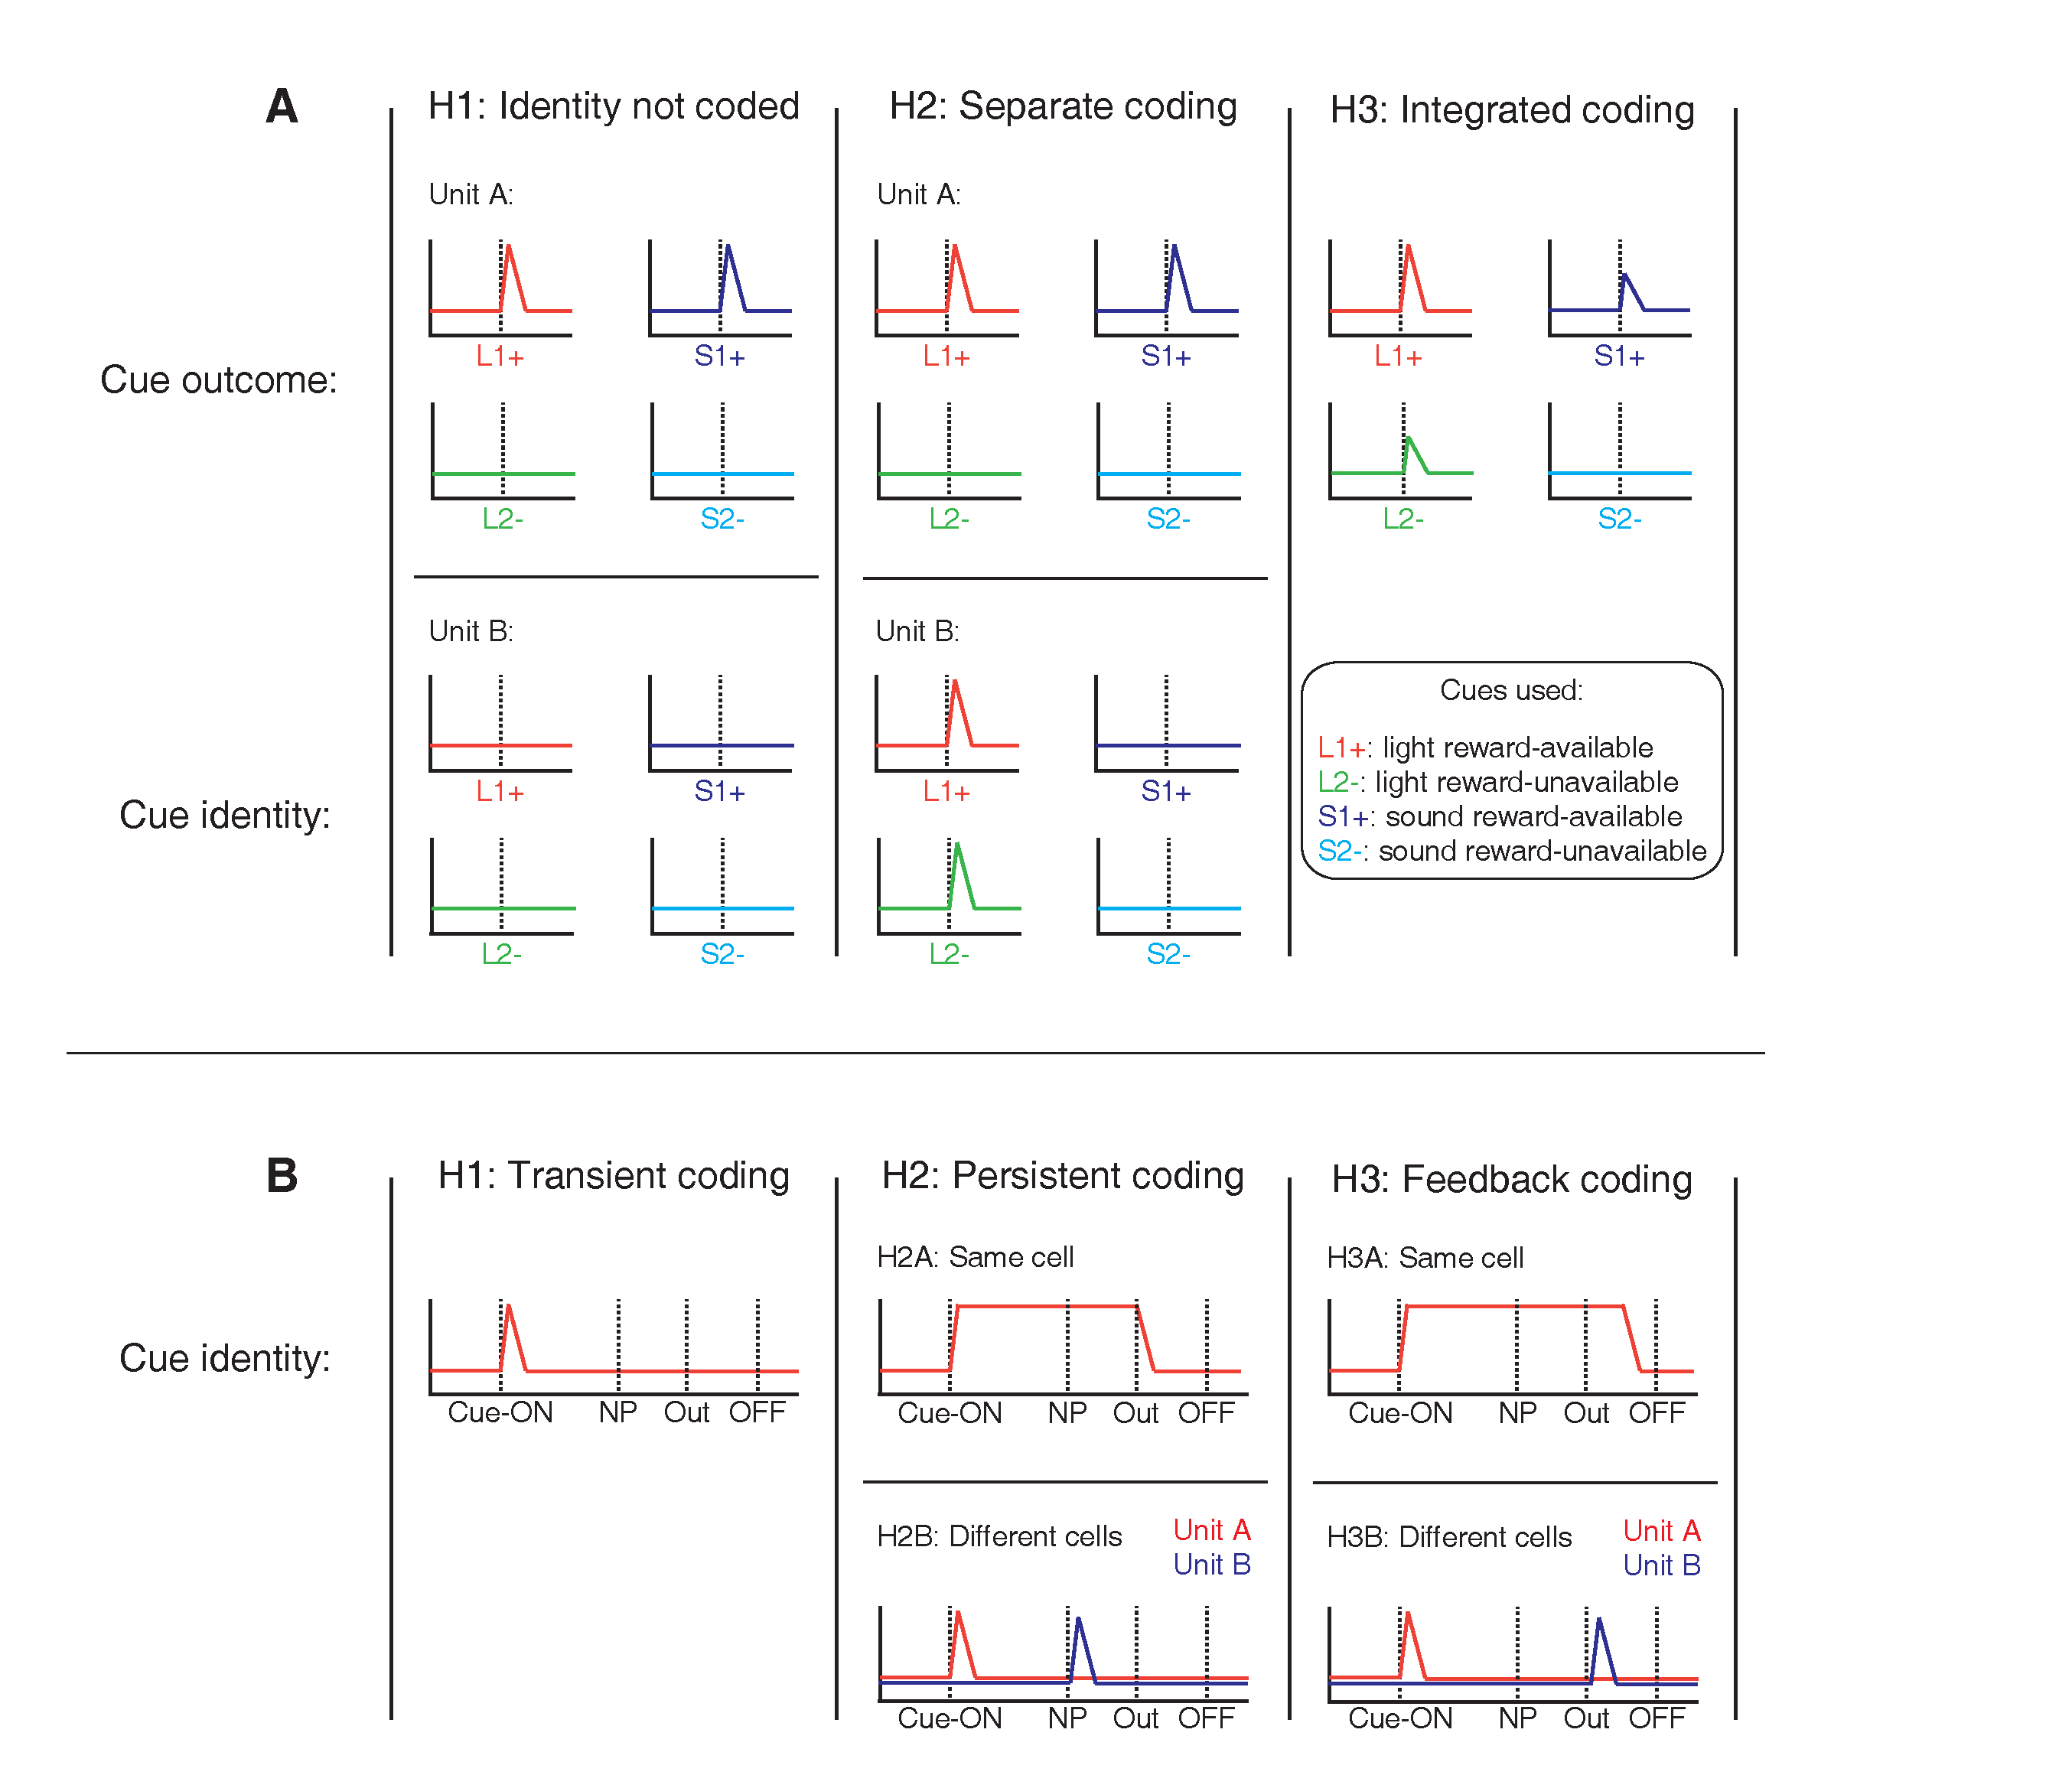
\includegraphics[height=0.5\textheight]{Fig 1 - Schematic neural.png}
\caption{Schematic of potential coding strategies \DIFaddbeginFL \DIFaddFL{for cue identity (light,
  sound) and cue outcome (reward-available, reward-unavailable) }\DIFaddendFL employed by
  single units in the NAc. \DIFdelbeginFL \DIFdelFL{Aim 1. }\DIFdelendFL \DIFaddbeginFL \DIFaddFL{\bsf{A}: }\DIFaddendFL Displayed are schematic PETHs illustrating
  putative responses to different cues under different hypotheses of how cue
  identity and value are coded. H1 (left panel): Coding of cue identity is
  absent in the NAc. Top: Unit A \DIFdelbeginFL \DIFdelFL{responds to }\DIFdelendFL \DIFaddbeginFL \DIFaddFL{encodes }\DIFaddendFL a motivationally relevant variable,
  such as expected outcome, similarly across other cue features, such as \DIFdelbeginFL \DIFdelFL{stimulus modality }\DIFdelendFL \DIFaddbeginFL \DIFaddFL{cue
  identity }\DIFaddendFL or physical location. Hypothetical plot is firing rate across
  time. \DIFdelbeginFL \DIFdelFL{Light}\DIFdelendFL \DIFaddbeginFL \DIFaddFL{L1}\DIFaddendFL + (red) signifies a reward-available light cue, \DIFdelbeginFL \DIFdelFL{Sound}\DIFdelendFL \DIFaddbeginFL \DIFaddFL{S1}\DIFaddendFL + (navy blue) a
  reward-available sound cue, \DIFdelbeginFL \DIFdelFL{Light- }\DIFdelendFL \DIFaddbeginFL \DIFaddFL{L2- }\DIFaddendFL (green) a reward-unavailable light cue, \DIFdelbeginFL \DIFdelFL{Sound- }\DIFdelendFL \DIFaddbeginFL \DIFaddFL{S2-
  }\DIFaddendFL (light blue) a reward-unavailable sound cue. Dashed line indicates onset of
  cue. Bottom: No units within the NAc discriminate their firing according to
  cue identity. H2 (middle panel): Coding of cue identity occurs independently
  of encoding of motivationally relevant variables \DIFdelbeginFL \DIFdelFL{like }\DIFdelendFL \DIFaddbeginFL \DIFaddFL{such as }\DIFaddendFL expected outcome or
  subsequent vigor. Top: Same as H1, with unit A discriminating between
  reward-available and reward-unavailable cues. Bottom: Unit B discriminates
  firing across stimulus modalities, depicted here as firing to light cues but
  not sound cues. H3 (right panel): Coding of cue identity is integrated with
  coding of other motivationally relevant variables. Hypothetical example
  demonstrating a unit that responds to reward-predictive cues, but firing rate
  is also modulated by \DIFdelbeginFL \DIFdelFL{stimulus modality}\DIFdelendFL \DIFaddbeginFL \DIFaddFL{cue identity}\DIFaddendFL , firing most for the reward-available light
  cue. \DIFdelbeginFL \DIFdelFL{Aim 2. }\DIFdelendFL \DIFaddbeginFL \DIFaddFL{\bsf{B}: }\DIFaddendFL Displayed are schematic PETHs illustrating potential ways in
  which cue identity \DIFdelbeginFL \DIFdelFL{is represented}\DIFdelendFL \DIFaddbeginFL \DIFaddFL{signals may persist over time}\DIFaddendFL . H1 (left panel): Cue-onset
  triggers a transient response to a unit that codes for cue identity. Dashed
  lines indicate time of a behavioral or environmental event. \DIFdelbeginFL \DIFdelFL{‘}\DIFdelendFL \DIFaddbeginFL \DIFaddFL{'}\DIFaddendFL Cue-ON\DIFdelbeginFL \DIFdelFL{’ }\DIFdelendFL \DIFaddbeginFL \DIFaddFL{' }\DIFaddendFL signifies
  onset of cue, \DIFdelbeginFL \DIFdelFL{‘}\DIFdelendFL \DIFaddbeginFL \DIFaddFL{'}\DIFaddendFL NP\DIFdelbeginFL \DIFdelFL{’ }\DIFdelendFL \DIFaddbeginFL \DIFaddFL{' }\DIFaddendFL signifies when the rat holds a nosepoke at a reward
  receptacle, \DIFdelbeginFL \DIFdelFL{‘}\DIFdelendFL \DIFaddbeginFL \DIFaddFL{'}\DIFaddendFL Out\DIFdelbeginFL \DIFdelFL{’ }\DIFdelendFL \DIFaddbeginFL \DIFaddFL{' }\DIFaddendFL signifies when the outcome is revealed, \DIFdelbeginFL \DIFdelFL{‘}\DIFdelendFL \DIFaddbeginFL \DIFaddFL{'}\DIFaddendFL Cue-OFF\DIFdelbeginFL \DIFdelFL{’ }\DIFdelendFL \DIFaddbeginFL \DIFaddFL{' }\DIFaddendFL signifies
  when the cue turns off. H2 (middle panel): Coding of cue identity is
  maintained during a nosepoke hold period until outcome is revealed. Coding can
  either be maintained by the same unit as during cue-onset (H2A) or by a
  sequence of units (H2B). H3 (right panel): Coding of cue identity is
  maintained during entire duration of cue, including after outcome is
  revealed. \DIFdelbeginFL \DIFdelFL{Same }\DIFdelendFL \DIFaddbeginFL \DIFaddFL{The same }\DIFaddendFL hypotheses \DIFdelbeginFL \DIFdelFL{applies }\DIFdelendFL \DIFaddbeginFL \DIFaddFL{apply }\DIFaddendFL to other information-containing aspects of
  the environment when the cue is presented, such as the physical location of
  the cue.}
\label{fig:schematic}
\end{figure}
\section*{Methods}

{\bf Subjects:}

Adult male Long-Evans rats (n = 4, Charles River, Saint Constant, QC) were used
as subjects. Rats were individually housed with a 12/12-h light-dark cycle, and
tested during the light cycle. Rats were food deprived to 85-90\% of their free
feeding weight (weight at time of implantation was 440 - 470 g), and water
restricted 4-6 hours before testing. All experimental procedures were approved
by the the University of Waterloo Animal Care Committee (protocol\# 11-06) and
carried out in accordance with Canadian Council for Animal Care (CCAC)
guidelines.

{\bf Overall timeline:}

Each \DIFdelbegin \DIFdel{subject }\DIFdelend \DIFaddbegin \DIFadd{rat }\DIFaddend was first handled for seven days during which they were exposed to the
\DIFdelbegin \DIFdel{running }\DIFdelend \DIFaddbegin \DIFadd{experiment }\DIFaddend room, the sucrose solution used as a reinforcer, and the click of the
\DIFdelbegin \DIFdel{valves upon approach to the receptacles. They }\DIFdelend \DIFaddbegin \DIFadd{sucrose dispenser valves. Rats }\DIFaddend were then shaped to run on the task for \DIFdelbegin \DIFdel{seven days where they were }\DIFdelend \DIFaddbegin \DIFadd{sucrose
reward while being }\DIFaddend restricted to running in the clockwise direction by
presenting a physical barrier to running counterclockwise. \DIFdelbegin \DIFdel{Rats then continued to be trained each day for 100 trials in both a light and sound block until approach behavior discriminated between reward-available and reward-unavailable cuesfor three consecutive days according to a chi square test, at which }\DIFdelend \DIFaddbegin \DIFadd{Cues signaling the
availability and inavailability of reward were then introduced (described in
detail below, and rats were trained for 200 trials per day until they
discriminated between the cues. At this }\DIFaddend point they underwent hyperdrive
implantation targeted at the NAc. Rats were allowed to recover for a minimum of
five days before being retrained on the task, and recording began once
performance returned to pre-surgery levels. Upon completion of recording,
animals were \DIFdelbegin \DIFdel{sacrificed }\DIFdelend \DIFaddbegin \DIFadd{euthanized }\DIFaddend and recording sites were histologically confirmed.

{\bf Behavioral task and training:}

Rats were trained to run clockwise on an elevated, square-shaped track (\DIFdelbegin \DIFdel{100x100 cm}\DIFdelend \DIFaddbegin \DIFadd{100 x
100 cm, track width 10 cm}\DIFaddend ) containing four possible reward locations (Figure
\ref{fig:task}). Rats initiated a \DIFdelbegin \DIFdel{trial }\DIFdelend \DIFaddbegin {\it \DIFadd{trial}} \DIFaddend by running down the length of an
arm, and triggering a photobeam located 24 cm from the start of each arm. Upon
trial initiation, \DIFdelbegin \DIFdel{a light or sound cue }\DIFdelend \DIFaddbegin \DIFadd{one of two possible light cues (L1, L2), or one of two
possible sound cues (S1, S2), }\DIFaddend was presented that signaled the presence (\DIFaddbegin {\it
  \DIFaddend reward-available trial\DIFaddbegin }\DIFadd{, L1+, S1+}\DIFaddend ) or absence (\DIFaddbegin {\it \DIFaddend reward-unavailable trial\DIFaddbegin }\DIFadd{,
L2-, S2-}\DIFaddend ) of a 12\% sucrose water reward (0.1 mL) at the upcoming \DIFaddbegin \DIFadd{reward }\DIFaddend site. A
trial was classified as an \DIFdelbegin \DIFdel{approach trial }\DIFdelend \DIFaddbegin {\it \DIFadd{approach trial}} \DIFaddend if the rat turned left at the
decision point and made a nosepoke at the reward receptacle (40 cm from the
decision point), while trials were classified as a \DIFdelbegin \DIFdel{skip trial }\DIFdelend \DIFaddbegin {\it \DIFadd{skip trial}} \DIFaddend if the rat
instead turned right at the decision point and triggered the photobeam to
initiate the \DIFdelbegin \DIFdel{following trial. In }\DIFdelend \DIFaddbegin \DIFadd{next trial. A trial is labeled }{\it \DIFadd{correct}} \DIFadd{if the rat approached
(i.e.\ nosepoked) on }\DIFaddend reward-available trials\DIFaddbegin \DIFadd{, and skipped (i.e.\ did not
nosepoke) on reward-unavailable trials. On reward-available trials }\DIFaddend there was a 1
second delay between a nosepoke and subsequent reward delivery. \DIFdelbegin \DIFdel{Trial length }\DIFdelend \DIFaddbegin {\it \DIFadd{Trial
  length}} \DIFaddend was determined by measuring the length of time from cue onset until
nosepoke (for approach trials), or from cue onset until the start of the
following trial (for skip trials). Trials could only be initiated through
clockwise progression through the series of arms, and each entry into the
subsequent arm on the track counted as a trial.
\DIFdelbegin \DIFdel{To get enough trials for neural analysis rats were trained each day in both a light and sound }\DIFdelend \DIFaddbegin 

\DIFadd{Each session consisted of both a }{\it \DIFadd{light }\DIFaddend block\DIFdelbegin \DIFdel{for }\DIFdelend \DIFaddbegin } \DIFadd{and a }{\it \DIFadd{sound block}} \DIFadd{with
}\DIFaddend 100 trials each. Within a block, one cue signaled reward was available on that
trial \DIFaddbegin \DIFadd{(L1+ or S1+)}\DIFaddend , while the other signaled reward was not available \DIFaddbegin \DIFadd{(L2- or
S2-)}\DIFaddend . Light block cues were a flashing white light, and a constant yellow
light. Sound block cues were a 2 kHz sine wave and a 8 kHz sine wave whose
amplitude was modulated from 0 to maximum by a 2 Hz sine wave. Reward-cue
associations were counterbalanced across rats\DIFdelbegin \DIFdel{. Cue }\DIFdelend \DIFaddbegin \DIFadd{, e.g.\ for some rats L1+ was the
flashing white light, and for others L1+ was the constant yellow light. The
order of cue }\DIFaddend presentation was pseudorandomized so that the same cue could not be
presented more than twice in a row. Block order within each day was also
pseudorandomized, such that the rat could \DIFaddbegin \DIFadd{not }\DIFaddend begin a session with the same
block for more than two days in a row. Each \DIFdelbegin \DIFdel{training or testing day }\DIFdelend \DIFaddbegin \DIFadd{session }\DIFaddend consisted of a 5 minute
pre-session period on a pedestal \DIFaddbegin \DIFadd{(a terracotta planter filled with towels)}\DIFaddend ,
followed by the first block, then the second block, then a 5 minute post-session
period on the pedestal. \DIFdelbegin \DIFdel{Performance was determined by the proportion of trials a rat approached each cue. Perfect performance would be 100\% approach on reward-available trials, and 0\% approach on reward-unavailable trials. }\DIFdelend Rats were trained daily until they could distinguish
between the reward-available and reward-unavailable cues for both light and
sound blocks for three consecutive days, according to a chi-square test
rejecting the null hypothesis of equal approaches for reward-available and
reward-unavailable trials, at which point they underwent \DIFaddbegin \DIFadd{eletrode implant
}\DIFaddend surgery.

\begin{figure}
[h]
\centering
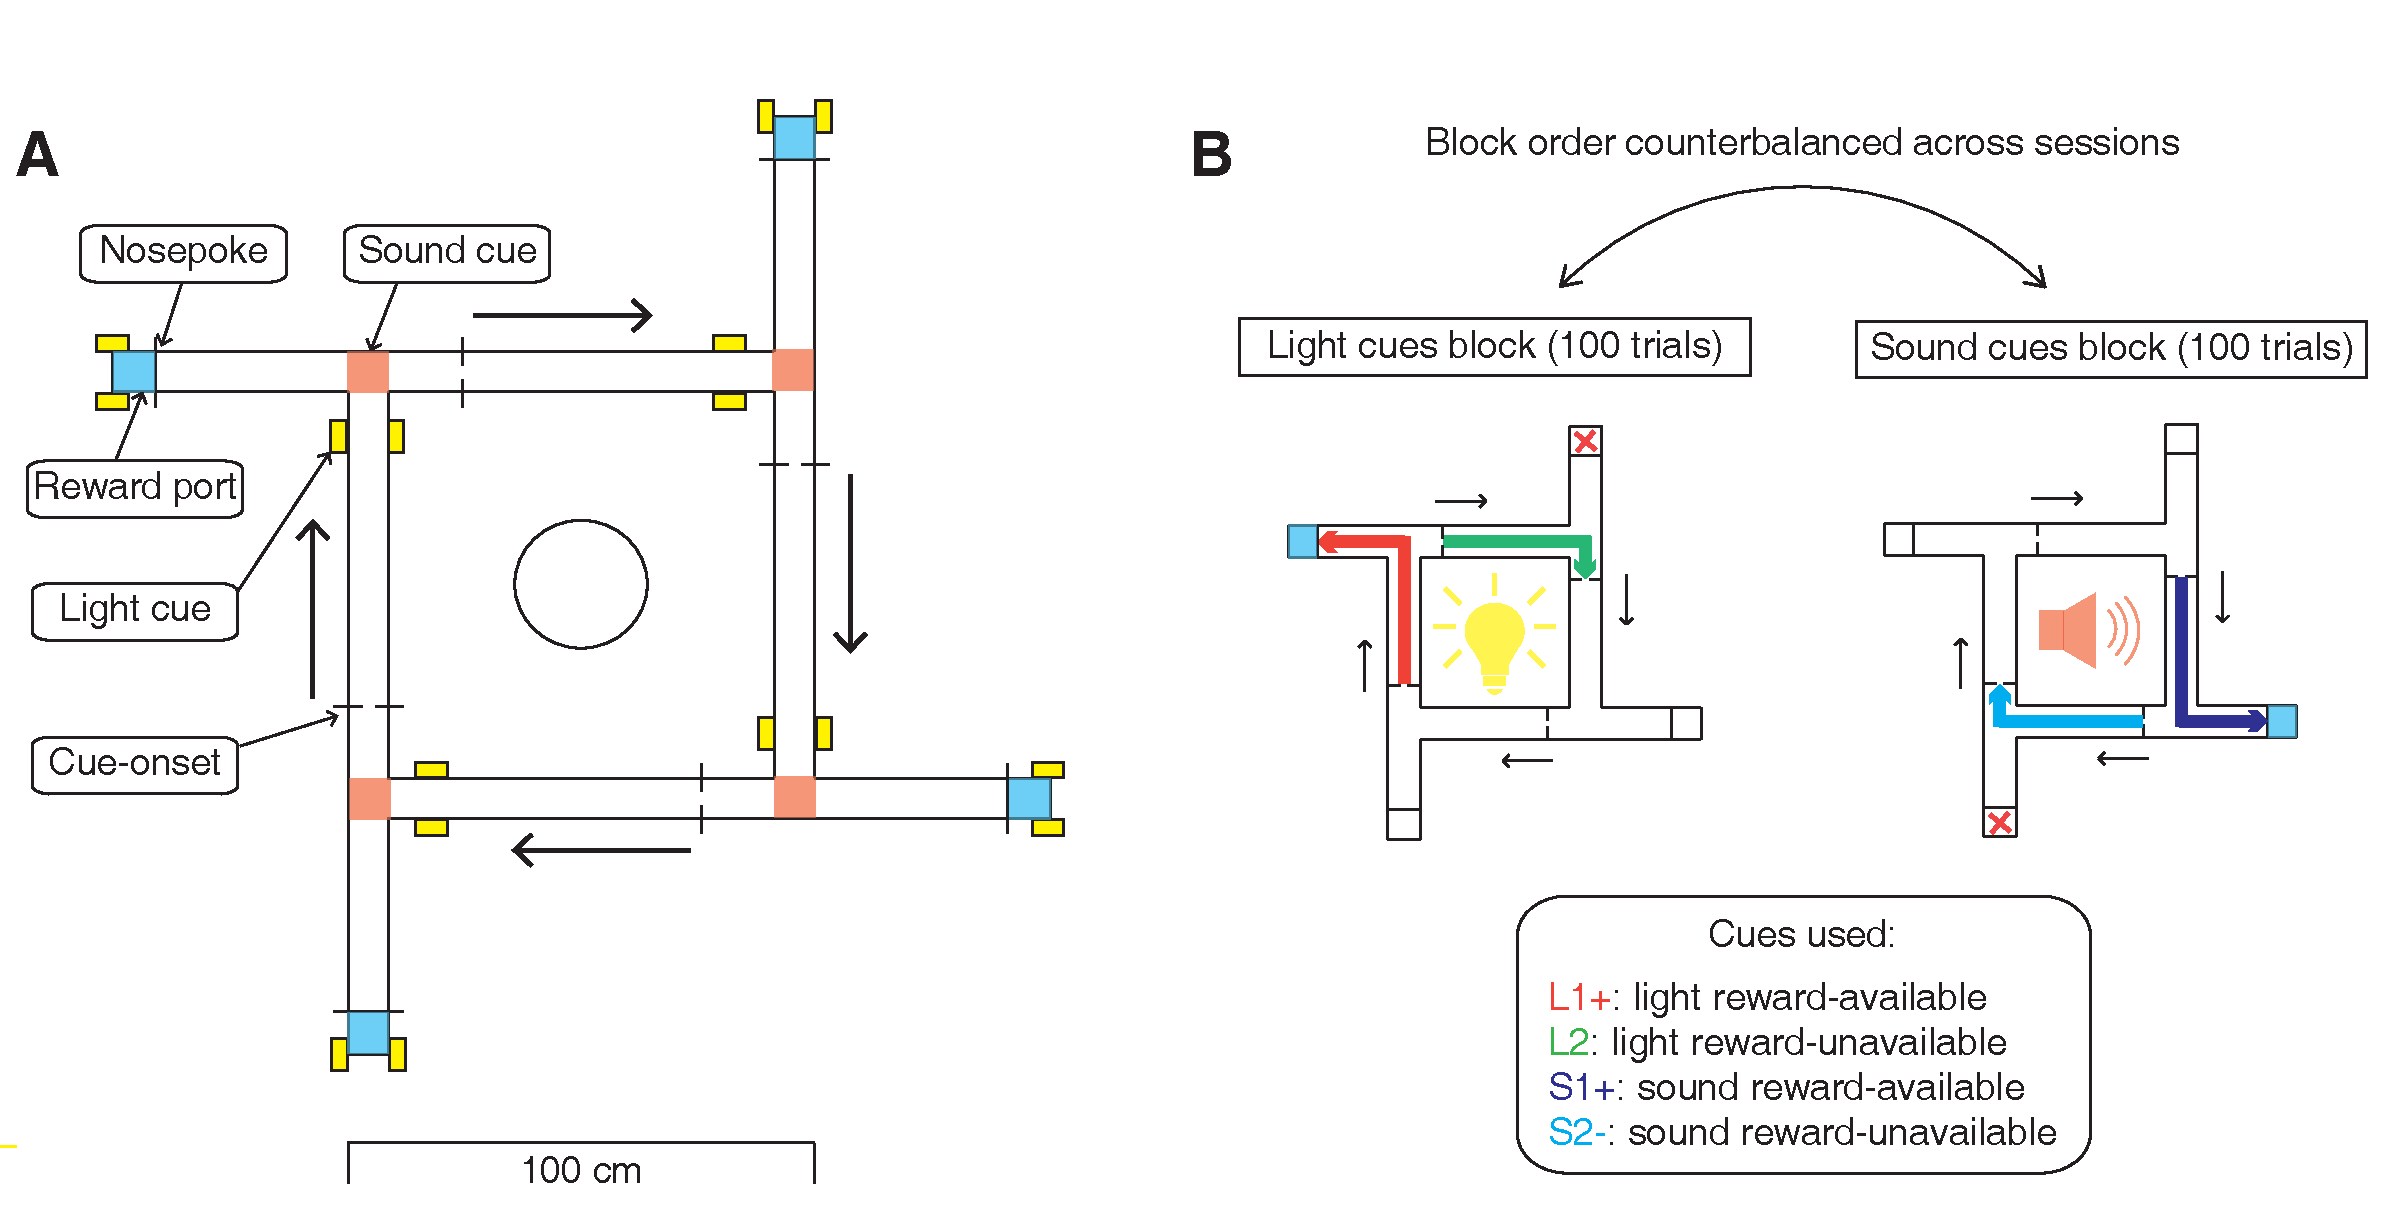
\includegraphics[width=\textwidth]{Fig 2 - Schematic task.png}
\caption{Schematic of behavioral task. \DIFdelbeginFL \DIFdelFL{A. }\DIFdelendFL \DIFaddbeginFL \DIFaddFL{\bsf{A}: }\DIFaddendFL To scale depiction of square
  track consisting of multiple identical T-choice points. \DIFdelbeginFL \DIFdelFL{Dashed lines indicate location of photobeams. Photobeams on the center}\DIFdelendFL \DIFaddbeginFL \DIFaddFL{At each choice point}\DIFaddendFL ,
  \DIFdelbeginFL \DIFdelFL{square portion }\DIFdelendFL \DIFaddbeginFL \DIFaddFL{the availability }\DIFaddendFL of \DIFaddbeginFL \DIFaddFL{sucrose reward at }\DIFaddendFL the \DIFdelbeginFL \DIFdelFL{track triggered the start }\DIFdelendFL \DIFaddbeginFL \DIFaddFL{nearest reward receptacle (light
  blue fill) was signaled by one }\DIFaddendFL of \DIFaddbeginFL \DIFaddFL{four possible cues, presented when the rat
  initiated }\DIFaddendFL a trial \DIFdelbeginFL \DIFdelFL{and onset of }\DIFdelendFL \DIFaddbeginFL \DIFaddFL{by crossing }\DIFaddendFL a \DIFdelbeginFL \DIFdelFL{cue, whereas photobeams }\DIFdelendFL \DIFaddbeginFL \DIFaddFL{photobeam on the track (dashed
  lines). Photobeams }\DIFaddendFL at the ends of the arms by the receptacles registered
  nosepokes. Rectangular boxes with yellow fill indicate location of LEDs used
  for light cues. Speakers for tone cues were placed underneath the choice
  points, indicated by magenta fill on track. Light blue fill on ends of arms
  indicate location of receptacles where sucrose was dispensed on rewarded
  trials. Circle in the center indicates location of pedestal during pre- and
  post-records. Scale bar is located beneath the track. \DIFdelbeginFL \DIFdelFL{B. }\DIFdelendFL \DIFaddbeginFL \DIFaddFL{\bsf{B}: }\DIFaddendFL Progression of
  a recording session. A session was started with a 5 minute recording period on
  a pedestal placed in the center of the apparatus. Rats then performed two
  blocks of a cue discrimination task on a square track where they had to
  dissociate between a reward-available and reward-unavailable cue for a set of
  light cues and a set of sound cues for a target of 100 trials each. Rats ran
  clockwise on the square track, and upon presentation of the cue could either
  turn left at the choice point to check if reward was available at the reward
  receptacle (approach trial; red and navy blue in figure), or turn right at the
  choice point to initiate the following trial (skip trial; green and light blue
  in figure). Reward-available and reward-unavailable cues were presented
  pseudo-randomly, such that not more than two of the same type of cue could be
  presented in a row. Location of the cue on the track was irrelevant for
  behavior, all cue locations contained an equal amount of reward-available and
  reward-unavailable trials. Left in figure depicts a light block, showing an
  example trajectory for a correct reward-available (red) and reward-unavailable
  (green) trial. Right in figure depicts a sound block, with a reward-available
  (navy blue) and reward-unavailable (light blue) trial. Ordering of the light
  and sound blocks was counterbalanced across sessions. Dashed line within track
  indicates photobeam that triggered cue onset. Solid line within track
  indicates photobeam that registered a nosepoke into the reward
  receptacles. Receptacles containing sucrose solution are present within the
  squares at the end of each arm. Light blue fill signifies reward receipt on a
  correct reward-available trial. Arrows outside of track indicate correct
  running direction. A session ended with another 5 minute recording period on
  the pedestal.}
\label{fig:task}

\end{figure}
{\bf Surgery:} 

Surgical procedures were as described previously (Malhotra et al.,
2015). Briefly, animals were \DIFaddbegin \DIFadd{administered analgesics and antibiotics,
}\DIFaddend anesthetized with isoflurane, induced with 5\% in medical grade oxygen and
maintained at 2\% throughout the surgery (~0.8 L/min). Rats were then
chronically implanted with a \DIFdelbegin \DIFdel{“hyperdrive” }\DIFdelend \DIFaddbegin \DIFadd{``hyperdrive'' }\DIFaddend consisting of 16 independently
drivable tetrodes, either all 16 targeted for the right NAc (AP +1.4 mm and ML
+1.6 mm \DIFdelbegin \DIFdel{, }\DIFdelend relative to bregma; Paxinos and Watson, 2005), or 12 in the right NAc
and 4 targeted at the mPFC (AP +3.0 mm and ML +0.6 mm, relative to bregma; only
data from NAc tetrodes \DIFdelbegin \DIFdel{were }\DIFdelend \DIFaddbegin \DIFadd{was }\DIFaddend analyzed). Following surgery, all animals were given
at least five days to recover \DIFdelbegin \DIFdel{and lower tetrodes
}\DIFdelend \DIFaddbegin \DIFadd{while receiving post-operative care, and tetrodes
were lowered }\DIFaddend to the target (DV -6.0 mm) before being reintroduced to the
behavioral task.

{\bf Data acquisition and preprocessing:}

After recovery, rats were placed back on the task for recording. NAc signals
were acquired at 20 kHz with a RHA2132 v0810 preamplifier (Intan) and a
KJE-1001/KJD-1000 data acquisition system (Amplipex). Signals were referenced
against a tetrode placed in the corpus callosum above the NAc. \DIFdelbegin %DIFDELCMD < 

%DIFDELCMD < %%%
\DIFdelend Candidate spikes
for sorting into putative single units were obtained by band-pass filtering the
data between 600-9000 Hz, thresholding and aligning the peaks (UltraMegaSort2k,
Hull et al., 2011). Spike waveforms were then clustered with KlustaKwik using
energy and the first derivative of energy as features, and manually sorted into
units (MClust 3.5, A.D.\DIFaddbegin \DIFadd{\ }\DIFaddend Redish et al.). Isolated units containing a minimum of
200 spikes within a session were included for subsequent analysis. Units were
classified as fast spiking interneurons (FSIs) by an absence of interspike
intervals (ISIs) $>$ 2 s, while medium spiny neurons (MSNs) had a combination of
ISIs $>$ 2 s and phasic activity with shorter ISIs (Barnes 2005, Atallah 2014).

{\bf Data analysis:}

\DIFdelbegin \DIFdel{For behavioral performance }\DIFdelend \DIFaddbegin {\it \DIFadd{Behavior.}} \DIFadd{To determine if rats distinguished behaviorally between the
reward-available and reward-unavailable cues (}{\it \DIFadd{cue outcome}}\DIFadd{), }\DIFaddend we generated
linear mixed effects models to investigate the relationships between cue type
and our behavioral variables, with \DIFdelbegin \DIFdel{cue type as a fixed effect}\DIFdelend \DIFaddbegin {\it \DIFadd{cue outcome}} \DIFadd{(reward available or not)
and }{\it \DIFadd{cue identity}} \DIFadd{(light or sound) as fixed effects}\DIFaddend , and the addition of an
intercept for rat identity as a random effect. \DIFdelbegin \DIFdel{Average }\DIFdelend \DIFaddbegin \DIFadd{For each cue, the average
}\DIFaddend proportion of trials approached and trial length for a session were used as
response variables. Contribution of cue \DIFdelbegin \DIFdel{type }\DIFdelend \DIFaddbegin \DIFadd{outcome }\DIFaddend to behavior was determined by
comparing the full model to a model with cue \DIFdelbegin \DIFdel{type }\DIFdelend \DIFaddbegin \DIFadd{outcome }\DIFaddend removed for each behavioral
variable.

\DIFaddbegin {\it \DIFadd{Neural data.}} \DIFaddend To investigate the contribution of \DIFdelbegin \DIFdel{various cue features
on NAc firing rates }\DIFdelend \DIFaddbegin \DIFadd{different cue features
}{\DIFadd{cue identity and cue outcome) on the firing rates of NAc single units, }\DIFaddend we first
  determined whether firing rates for a unit were modulated by the onset of a
  cue by collapsing across all cues and comparing the firing rates for the 1 s
  preceding cue-onset with the 1 s following cue-onset. Single units were
  considered to be \DIFdelbegin \DIFdel{cue-responsive }\DIFdelend \DIFaddbegin {\it \DIFadd{cue-modulated}} \DIFaddend if a Wilcoxon signed-rank test comparing
  pre- and post-cue firing \DIFdelbegin \DIFdel{had a p $<$ }\DIFdelend \DIFaddbegin \DIFadd{was significant at $p <$ }\DIFaddend .01. \DIFdelbegin \DIFdel{(Excluded: ‘the mean firing rate difference between pre- and post-cue onset was within the lower or upper 2.5\% of a shuffled distribution’, as there is redundancy using both, and I did both because I was paranoid about just using one. ). }\DIFdelend Cue-modulated units
  were then classified as either increasing or decreasing \DIFdelbegin \DIFdel{in response to the cue }\DIFdelend if the post-cue
  activity was higher or lower than the pre-cue activity, respectively.

To determine the relative contribution of \DIFdelbegin \DIFdel{various }\DIFdelend \DIFaddbegin \DIFadd{different }\DIFaddend task parameters to firing
rate variance \DIFdelbegin \DIFdel{for units whose firing was modulated by cue-onset }\DIFdelend (as in Figures \ref{fig:examples}\DIFdelbegin \DIFdel{,}\DIFdelend \DIFaddbegin \DIFadd{-}\DIFaddend \ref{fig:GLM}), a forward
selection stepwise general linear model (GLM) was fit to each \DIFdelbegin \DIFdel{cue-responsive }\DIFdelend \DIFaddbegin \DIFadd{cue-modulated
}\DIFaddend unit. Cue identity (light block, sound block), cue location (arm 1, arm 2, arm
3, arm 4), cue outcome (reward-available, reward-unavailable), \DIFdelbegin \DIFdel{approach behavior
, }\DIFdelend \DIFaddbegin \DIFadd{behavior
(approach, skip), }\DIFaddend trial length, trial number, and trial history \DIFaddbegin \DIFadd{(reward
availability on the previous 2 trials) }\DIFaddend were used as predictors, and the 1 s
post-cue firing rate as the response variable. Units were classified as being
modulated by a given task parameter if addition of the parameter significantly
improved model fit using deviance as the criterion (\DIFdelbegin \DIFdel{p $<$ }\DIFdelend \DIFaddbegin \DIFadd{$p <$ }\DIFaddend .01). A comparison of
the R-squared value between the final model and the final model minus the
predictor of interest was used to determine the amount of firing rate variance
explained by the addition of that predictor for a given unit.

To better visualize responses to cues and enable subsequent population level
analyses (as in Figures \ref{fig:examples}, \ref{fig:pop}, \DIFaddbegin \DIFadd{and
}\DIFaddend \ref{fig:tiling}), spike trains were convolved with a Gaussian kernel ($\sigma$
= 100 ms), and peri-event time histograms (PETHs) were generated by taking the
average of the convolved spike trains across trials for a given task
condition. For analysis of population-level responses for cue features (Figure
\ref{fig:pop}), convolved spike trains for all units where cue identity, cue
location, or cue outcome explained a significant portion of firing rate variance
were z-scored. Within a given cue feature, normalized spike trains were then
separated according to the preferred and non-preferred cue condition
(e.g.\DIFdelbegin \DIFdel{light vs }\DIFdelend \DIFaddbegin \DIFadd{\ light vs.\ }\DIFaddend sound block), and averaged across units to generate
population-level averages. To account for separation that would result from any
random selection of units, cell identity was shuffled and the shuffled average
for \DIFdelbegin \DIFdel{preferrend }\DIFdelend \DIFaddbegin \DIFadd{preferred }\DIFaddend and non-preferred cue conditions was generated for 1000 shuffles.

To visualize NAc representations of task space within cue conditions, normalized
spike trains for all units were ordered by the location of their maximum or
minimum firing rate for a specified cue condition (Figure \ref{fig:tiling}). To
compare representations of task space across cue conditions for a cue feature,
the ordering of units derived for one condition (e.g.\ light block) was then
applied to the normalized spike trains for the other condition (e.g.\ sound
block). For control comparisons within cue conditions, half of the trials for a
condition were compared against the other half. To look at the correlation of
firing rates of all cells within and across various cue conditions, trials for
each cue condition for a cell were shuffled and divided into two averages, and
averages within and across cue conditions were correlated. A linear mixed
effects model was run for each cue condition to determine if correlations of
firing rates within cue conditions were more similar than correlations across
cue conditions.

To identify the responsivity of units to different cue features at the time of a
nosepoke into a reward receptacle, and subsequent reward delivery, the same
cue-responsive units from the cue-onset analyses were analyzed at the time of
nosepoke and reward receipt using identical analysis techniques (Figures
\ref{fig:NP_examples}, \ref{fig:NP_GLM}, \ref{fig:NP_pop}, \DIFaddbegin \DIFadd{and
}\DIFaddend \ref{fig:NP_tiling}).

Given that some of our analyses compare firing rates across time, particularly
comparisons across blocks, we sought to exclude units with unstable firing rates
that would generate spurious results reflecting a drift in firing rate over time
unrelated to our task. To do this we ran a Mann-Whitney U test comparing the
cue-evoked firing rates for the first and second half of trials within a block,
and excluded 99 units from analysis that showed a significant change for either
block. All analyses were completed in MATLAB R2015a, the code is available on
our public GitHub repository (http://github.com/vandermeerlab/papers), and the
data can be accessed through DataLad.

{\bf Histology:}

Upon completion of the experiment, rats were anesthetized with 5\% isoflurane,
then asphyxiated with carbon dioxide. Transcardial perfusions were performed,
and brains were fixed and removed. Brains were sliced in 50 $\mu m$ coronal
sections and stained with thionin. Slices were visualized under light
microscopy, tetrode placement was determined, and electrodes with recording
locations in the NAc were analyzed (Figure \ref{fig:histo}).

\begin{figure}[h]
\centering
\includegraphics[width=\textwidth]{Fig 3 - Histology.png}
\caption{Histological verification of recording sites. Upon completion of
  experiments, brains were sectioned and tetrode placement was
  confirmed. \DIFdelbeginFL \DIFdelFL{A. }\DIFdelendFL \DIFaddbeginFL \DIFaddFL{\bsf{A}: }\DIFaddendFL Example section from R060 showing a recording site in the
  NAc core just dorsal to the anterior commissure (white circle). \DIFdelbeginFL \DIFdelFL{B. }\DIFdelendFL \DIFaddbeginFL \DIFaddFL{\bsf{B}:
  }\DIFaddendFL Schematic showing recording areas for the four rats used\DIFdelbeginFL \DIFdelFL{in the present study}\DIFdelendFL .\DIFdelbeginFL \DIFdelFL{.}\DIFdelendFL }
\label{fig:histo}
\end{figure}
\section*{Results}

\subsection*{Behavior}

Rats were trained to discriminate between cues signaling the availability and
absence of reward on a square track with four identical arms for two distinct
sets of cues \DIFaddbegin \DIFadd{(Figure \ref{fig:task})}\DIFaddend . During each session, rats were presented
sequentially with two behavioral blocks containing cues from different sensory
modalities, a light and a sound block, with each block containing a cue that
signalled the availability of reward (reward-available), and a cue that
signalled the absence of reward (reward-unavailable). \DIFdelbegin \DIFdel{An example learning curve is seen in }\DIFdelend \DIFaddbegin \DIFadd{To maximize reward
receipt, rats should approach reward sites on reward-available trials, and skip
reward sites on reward-unavailable trials (see }\DIFaddend Figure \ref{fig:behav}A \DIFdelbegin \DIFdel{,B}\DIFdelend \DIFaddbegin \DIFadd{for an
example learning curve)}\DIFaddend . All four rats learned to discriminate between the
reward-available and reward-unavailable cues for both the light and sound blocks
as determined by reaching significance (\DIFdelbegin \DIFdel{p $<$ }\DIFdelend \DIFaddbegin \DIFadd{$p <$ }\DIFaddend .05) on a daily chi-square test
comparing approach behavior for reward-available and reward-unavailable cues for
each block, for at least three consecutive days (range for time to criterion: 22
- 57 days). Maintenance of behavioral performance during recording sessions was
assessed using linear mixed effects models for both proportion of trials where
the rat approached the receptacle, and trial length. Analyses revealed that the
likelihood of a rat to make an approach was influenced by which of the cues was
presented (Percentage approached: light reward-available = 97\%; light
reward-unavailable = 34\%; sound reward-available = 91\%; sound
reward-unavailable 35\%; p $<$ .001), but that cue identity did not
significantly affect the length of time taken to complete a trial (Trial length:
light reward-available = 1.85 s; light reward-unavailable = 1.74 s; sound
reward-available = 1.91 s; sound reward-unavailable 1.78 s; p $=$ .13\DIFdelbegin \DIFdel{)(}\DIFdelend \DIFaddbegin \DIFadd{; }\DIFaddend Figure
\ref{fig:behav}C,D). Thus, during recording, rats successfully discriminated the
\DIFdelbegin \DIFdel{various }\DIFdelend cues according to whether or not they \DIFdelbegin \DIFdel{signalled }\DIFdelend \DIFaddbegin \DIFadd{signaled }\DIFaddend the availability of reward at the
reward receptacle.

\begin{figure}[h]
\centering
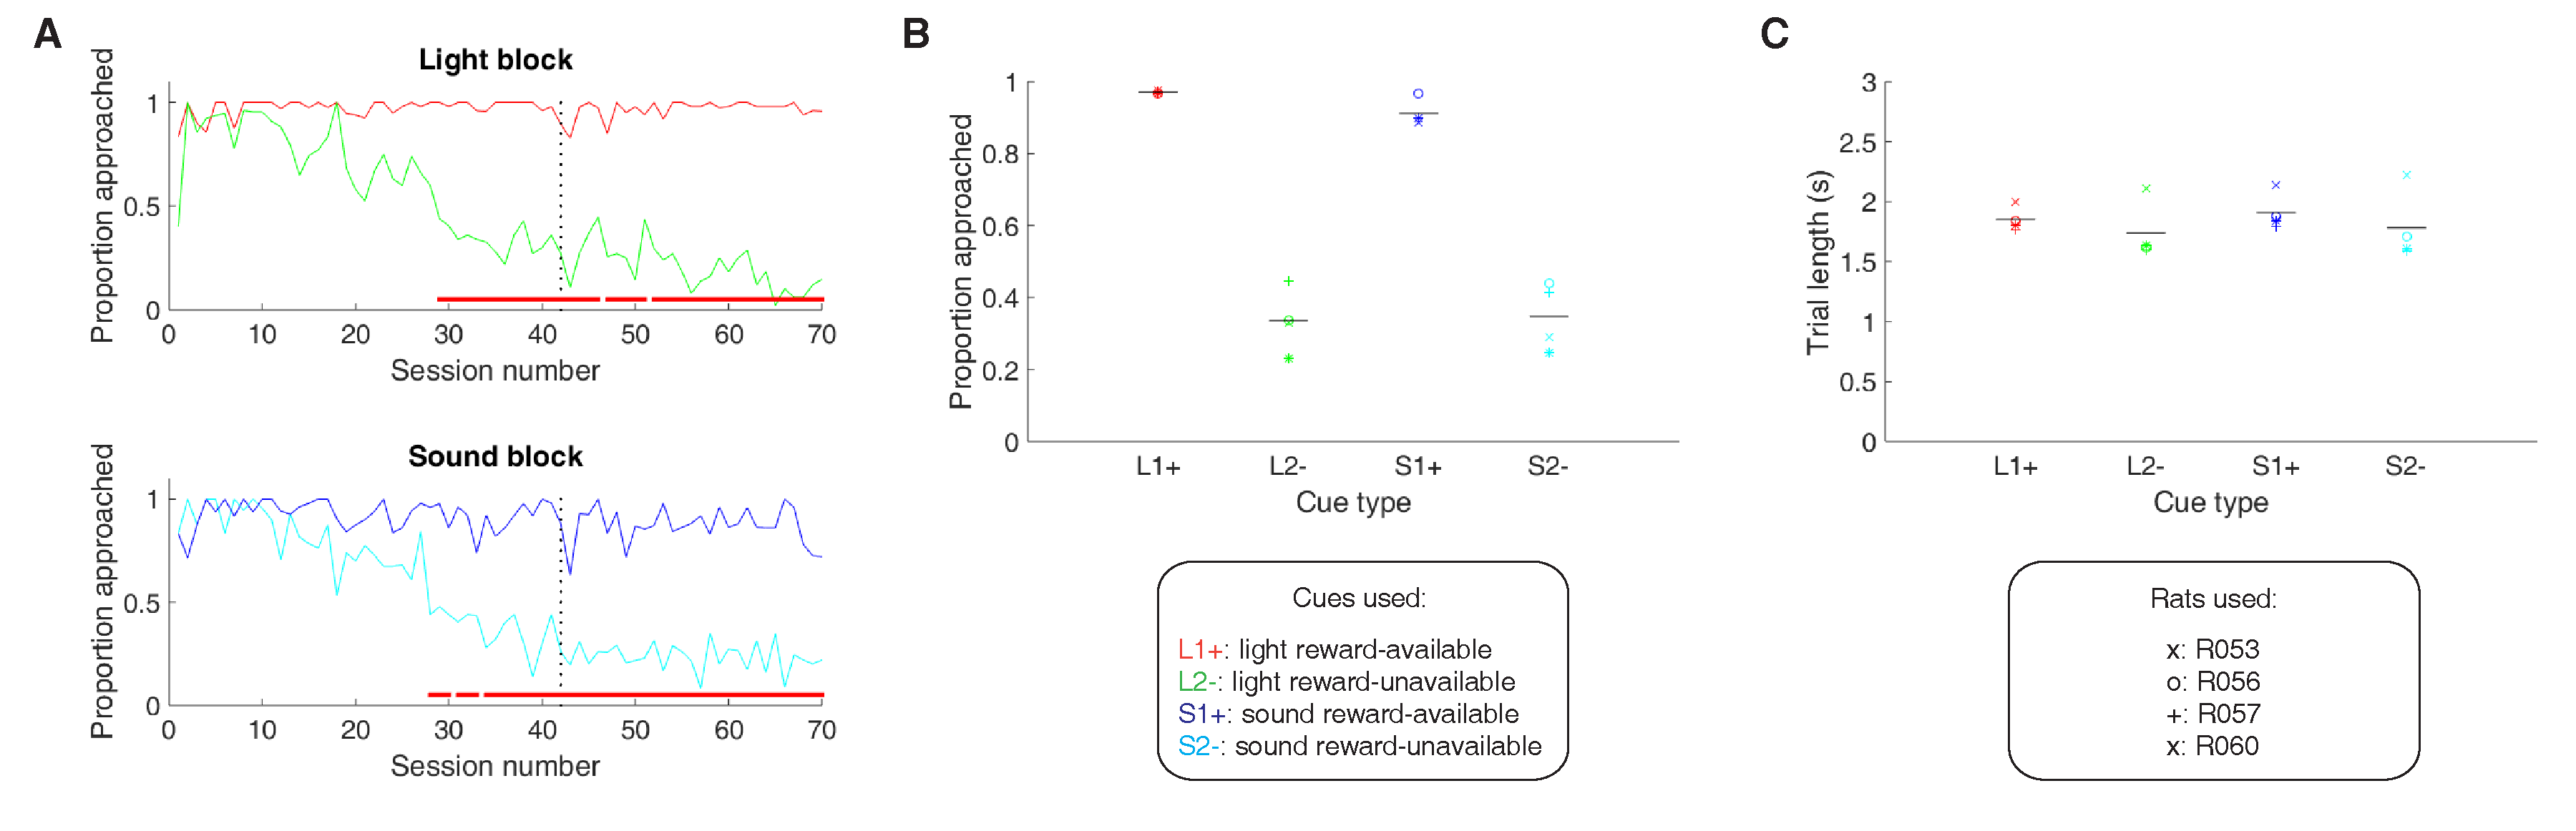
\includegraphics[width=\textwidth]{Fig 4 - Behavioral results.png}
\caption{Performance on the behavioral task. \DIFdelbeginFL \DIFdelFL{A-B}\DIFdelendFL \DIFaddbeginFL \DIFaddFL{\bsf{A-B}}\DIFaddendFL . Example learning curves
  across sessions from a single subject (R060) showing the proportion approached
  for reward-available (red line for light block, navy blue line for sound
  block) and reward-unavailable trials (green line for light block, light blue
  line for sound block). Fully correct performance corresponds to approach
  proportion of 1 for reward-available trials and 0 for reward-unavailable
  trials. Rats initially \DIFdelbeginFL \DIFdelFL{start out approaching }\DIFdelendFL \DIFaddbeginFL \DIFaddFL{approach }\DIFaddendFL on both reward-available and
  reward-unavailable trials, and learn with experience to skip non-rewarded
  trials. Red bars indicate days in which a rat statistically discriminated
  between reward-available and reward-unavailable cues, determined by a chi
  square test. Dashed line indicates time of electrode implant
  surgery. \DIFdelbeginFL \DIFdelFL{C-D. }\DIFdelendFL \DIFaddbeginFL \DIFaddFL{\bsf{C-D}: }\DIFaddendFL Summary of performance during recording sessions for each
  rat. \DIFdelbeginFL \DIFdelFL{C. }\DIFdelendFL \DIFaddbeginFL \DIFaddFL{\bsf{C}: }\DIFaddendFL Proportion approached for all rats, averaged across all
  recording sessions. Different columns indicate the different cues
  (reward-available (red) and reward-unavailable (green) light cues,
  reward-available (navy blue) and reward-unavailable (light blue) sound
  cues). Different symbols correspond to individual subjects; horizontal black
  line shows the mean. All rats learned to discriminate between reward-available
  and reward-unavailable cues, as indicated by the clear difference of
  proportion approached between reward-available ($\sim$90\% approached) and
  reward-unavailable cues ($\sim$30\% approached), for both blocks (see Results
  for statistics). \DIFdelbeginFL \DIFdelFL{D. }\DIFdelendFL \DIFaddbeginFL \DIFaddFL{\bsf{D}: }\DIFaddendFL Average trial length for each cue. Note that the
  time to complete a trial was comparable for the different cues.}
\label{fig:behav}
\end{figure}
\subsection*{NAc neurons encode behaviorally relevant and irrelevant cue features}

{\bf Single unit responses discriminate cue features:}

We sought to address which parameters of our task were encoded by NAc activity,
specifically whether the NAc encodes aspects of motivationally relevant cues not
directly tied to reward, such as the identity and location of the cue, and
whether this coding is independent or integrated with coding of cue outcome. To
do this we recorded a total of 443 units with $>$ 200 spikes in the NAc from 4
rats over 57 sessions while they performed a cue discrimination task (Table
\ref{tbl1}). Units that exhibited a drift in firing rate over the course of
either block were excluded from further analysis, leaving 344 units for further
analysis. The activity of 133 (39\%) of these 344 units were modulated by the
cue, with more showing a decrease in firing (n = 103) than an increase (n = 30)
around the time of cue-onset (Table \DIFdelbegin \DIFdel{\ref{tbl2}}\DIFdelend \DIFaddbegin \DIFadd{\ref{tbl1}}\DIFaddend ). Within this group, 24 were
classified as FSIs, while 109 were classified as SPNs. Upon visual inspection,
we observed several patterns of firing activity, including units that
\DIFdelbegin \DIFdel{; }\DIFdelend discriminated firing upon cue-onset across various cue conditions, showed
sustained differences in firing across cue conditions, had transient responses
to the cue, showed a ramping of activity starting at cue-onset, and showed
elevated activity immediately preceding cue-onset, for example (Figure
\ref{fig:examples}). To characterize more formally whether these cue-evoked
responses were modulated by various aspects of the task, we fit a GLM to each
cue-modulated unit. Fitting GLMs revealed that a variety of task parameters
accounted for a significant portion of firing rate variance in NAc cue-modulated
units (Figure \ref{fig:GLM}, Table \DIFdelbegin \DIFdel{\ref{tbl2}}\DIFdelend \DIFaddbegin \DIFadd{\ref{tbl1}}\DIFaddend ). Notably, there were units that
discriminated between whether the rat was performing in the light or sound block
(28\% of cue-modulated units, accounting for 6\% of variance on average), which
arm the rat was currently on (38\% of cue-modulated units, accounting for 6\% of
variance on average), and whether the rat was engaged in the common portion of a
reward-available or reward-unavailable trial (26\% of cue-modulated units,
accounting for 4\% of variance on average), suggesting that the NAc
independently encodes features of reward-predictive cues separate from expected
outcome (Figure \ref{fig:examples}A-F). Furthermore, \DIFdelbegin \DIFdel{interactions between multiple cue features appeared as significant predictors of firing rate variance for 8\% of cue-modulated units , although this effect was modest ($\sim$1-2\% variance explained), suggesting a weak effect }\DIFdelend \DIFaddbegin \DIFadd{overlap of coding of cue
features within units was not different than expected by chance according to
chi-square tests, suggesting }\DIFaddend for integrated coding across various aspects of a
cue (Figure \ref{fig:examples}G,H). Fitting a GLM to all recorded units revealed
a similar pattern of results (data not shown). Together, these findings show
that various cue features are represented in the NAc, and that this coding has
some overlap, but is mostly distinct from expected outcome (Figure
\ref{fig:schematic}; H2,H3).


\begin{table}
[p]
\centering
\setlength{\tabcolsep}{1 em} % for the horizontal padding
\begin{tabular}{l c  c c c c}

\DIFdelbeginFL \DIFdelFL{Rat                                   }\DIFdelendFL \DIFaddbeginFL \DIFaddFL{Task parameter                                 }\DIFaddendFL & Total        & $\uparrow$ MSN        & $\downarrow$ MSN        & $\uparrow$ FSI       & $\downarrow$ FSI\\
\hline
\DIFaddbeginFL \DIFaddFL{All units                       }& \DIFaddFL{443        }& \DIFaddFL{155         }& \DIFaddFL{216          }& \DIFaddFL{27          }& \DIFaddFL{45}\\
\hline
\DIFaddFL{Rat ID                       }&         &       &          &          &\\
\hline
\DIFaddendFL R053                       & 145         & 51          & 79          & 4         & 11\\
\hline
R056                       & 70         & 12          & 13         & 17          & 28\\
\hline
R057   	          & 136         & 55          & 75          & 3          & 3\\
\hline
R060                       & 92         & 37          & 49          & 3          & 3\\
\hline 
\DIFdelbeginFL %DIFDELCMD < 

%DIFDELCMD < \end{tabular}
%DIFDELCMD < \caption {%%%
\DIFdelFL{Cells from each rat}%DIFDELCMD < } %DIFDELCMD < \label{tbl1} %%%
%DIFDELCMD < \end{table}
%DIFDELCMD < 

%DIFDELCMD < \begin{table}[p]
%DIFDELCMD < \centering
%DIFDELCMD < \setlength{\tabcolsep}{1 em} %%%
%DIF <  for the horizontal padding
%DIFDELCMD < \begin{tabular}{l c  c c c c}
%DIFDELCMD < 

%DIFDELCMD < %%%
\DIFdelFL{Task parameter                                 }%DIFDELCMD < & %%%
\DIFdelFL{Total        }%DIFDELCMD < & %%%
\DIFdelFL{$\uparrow$ MSN        }%DIFDELCMD < & %%%
\DIFdelFL{$\downarrow$ MSN        }%DIFDELCMD < & %%%
\DIFdelFL{$\uparrow$ FSI       }%DIFDELCMD < & %%%
\DIFdelFL{$\downarrow$ FSI}%DIFDELCMD < \\
%DIFDELCMD < \hline
%DIFDELCMD < %%%
\DIFdelFL{All units                       }%DIFDELCMD < & %%%
\DIFdelFL{443        }%DIFDELCMD < & %%%
\DIFdelFL{155         }%DIFDELCMD < & %%%
\DIFdelFL{216          }%DIFDELCMD < & %%%
\DIFdelFL{27          }%DIFDELCMD < & %%%
\DIFdelFL{45}%DIFDELCMD < \\
%DIFDELCMD < \hline
%DIFDELCMD < %%%
\DIFdelendFL Analyzed units                       & 344        & ?         & ?         & ?          & ?\\
\hline
Cue modulated units                      & 133         &24          &85          & 6          &18\\
\hline
GLM aligned to cue-onset                       &         &       &          &          &\\
\hline
Cue identity       & 37         & 7          & 21          & 1          & 8\\
\hline
Cue location       & 50         &13          & 27          & 3          & 7\\
\hline
Cue outcome       & 34         & 10          & 18        & 0          & 6\\
\hline
Approach behavior      & 31         & 8          & 18          & 1          & 4\\
\hline
Trial length       & 25        & 5          & 18         & 0         & 2\\
\hline
Trial number       & 32         & 11          & 12         & 1          & 8\\
\hline
Recent trial history       & 5         & 0          &5          & 0          & 0\\
\hline
\DIFdelbeginFL \DIFdelFL{Cue x cue interactions       }%DIFDELCMD < & %%%
\DIFdelFL{11         }%DIFDELCMD < & %%%
\DIFdelFL{3          }%DIFDELCMD < & %%%
\DIFdelFL{7          }%DIFDELCMD < & %%%
\DIFdelFL{0          }%DIFDELCMD < & %%%
\DIFdelFL{1}%DIFDELCMD < \\
%DIFDELCMD < \hline
%DIFDELCMD < %%%
\DIFdelFL{Cue x behavior interactions       }%DIFDELCMD < & %%%
\DIFdelFL{?         }%DIFDELCMD < & %%%
\DIFdelFL{?          }%DIFDELCMD < & %%%
\DIFdelFL{?          }%DIFDELCMD < & %%%
\DIFdelFL{?          }%DIFDELCMD < & %%%
\DIFdelFL{?}%DIFDELCMD < \\
%DIFDELCMD < \hline
%DIFDELCMD < %%%
\DIFdelendFL GLM aligned to nosepoke                       &         &       &          &          &\\
\hline
Cue identity       & 66         &14          & 36          & 2          &14\\
\hline
Cue location       & 66         &14          & 40          & 3          & 9\\
\hline
Cue outcome       & 42        & 8          & 29        & 0          & 5\\
\hline
GLM aligned to outcome                       &         &       &          &          &\\
\hline
Cue outcome       & 10        & 0          & 6       & 0          &4\\
\hline

\end{tabular}
\caption {Cells \DIFdelbeginFL \DIFdelFL{from GLM}\DIFdelendFL \DIFaddbeginFL \DIFaddFL{overview}\DIFaddendFL } \DIFdelbeginFL %DIFDELCMD < \label{tbl2} 
%DIFDELCMD < %%%
\DIFdelendFL \DIFaddbeginFL \label{tbl1} 
\DIFaddendFL \end{table}

\begin{figure}[h]
\centering
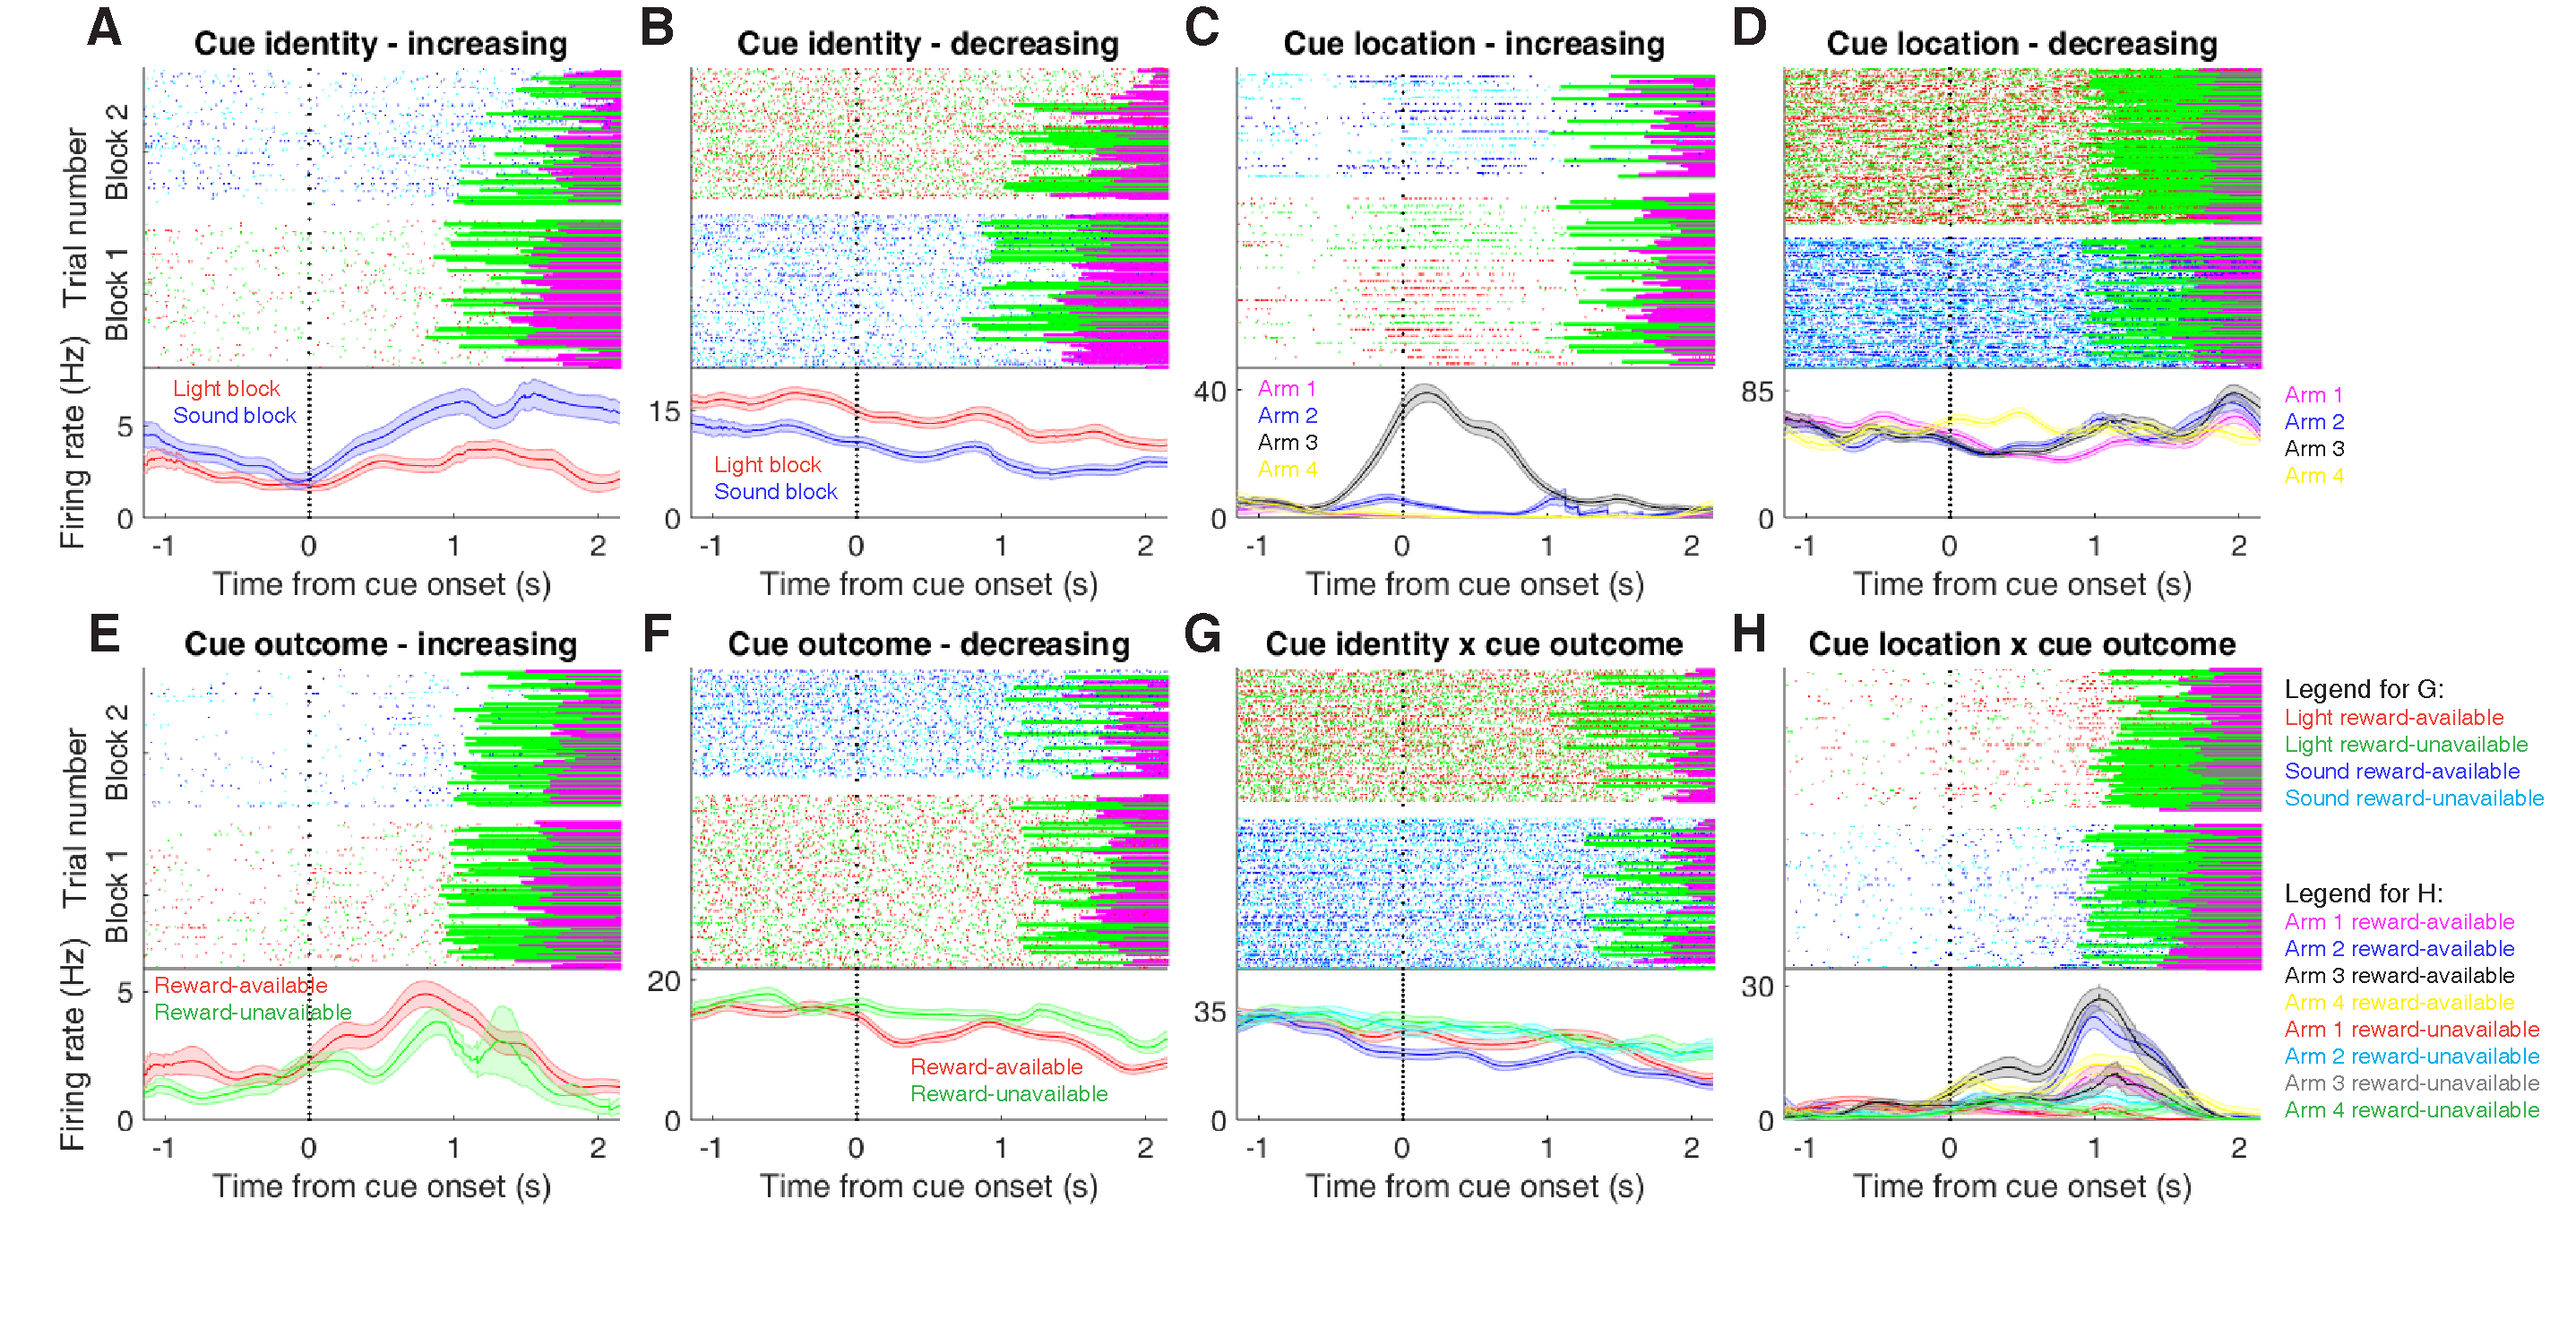
\includegraphics[width=\textwidth]{Fig 5 - Neural examples.png}
\caption{Examples of different cue-modulated NAc units influenced by various
  task parameters. \DIFdelbeginFL \DIFdelFL{A. }\DIFdelendFL \DIFaddbeginFL \DIFaddFL{\bsf{A}: }\DIFaddendFL Example of a cue-modulated NAc unit that showed an
  increase in firing \DIFdelbeginFL \DIFdelFL{in response to }\DIFdelendFL \DIFaddbeginFL \DIFaddFL{following }\DIFaddendFL the cue, and encoded cue identity. Top:
  rasterplot showing the spiking activity across all trials aligned to
  cue-onset. Spikes across trials are \DIFdelbeginFL \DIFdelFL{color coded }\DIFdelendFL \DIFaddbeginFL \DIFaddFL{color-coded }\DIFaddendFL according to cue type (red:
  reward-available light; green: reward-unavailable light; navy blue:
  reward-available sound; light blue: reward-unavailable sound). Green and
  magenta bars indicate trial termination when a rat initiated the next trial or
  made a nosepoke, respectively. White space halfway up the rasterplot indicates
  switching from one block to the next. Dashed line indicates cue onset. Bottom:
  PETHs showing the average smoothed firing rate for the unit for trials during
  light (red) and sound (blue) blocks, aligned to cue-onset. Lightly shaded area
  indicates standard error of the mean. Note this unit showed a larger increase
  in firing to sound cues. \DIFdelbeginFL \DIFdelFL{B. }\DIFdelendFL \DIFaddbeginFL \DIFaddFL{\bsf{B}: }\DIFaddendFL An example of a unit that was responsive to
  cue identity as in A, but for a unit that showed a decrease in firing to the
  cue. Note the sustained higher firing rate during the light block. \DIFdelbeginFL \DIFdelFL{C-D. }\DIFdelendFL \DIFaddbeginFL \DIFaddFL{\bsf{C-D}:
  }\DIFaddendFL Cue-modulated units that encoded cue location, each color in the PETHs
  represents average firing response for a different cue location. \DIFdelbeginFL \DIFdelFL{C. This }\DIFdelendFL \DIFaddbeginFL \DIFaddFL{\bsf{C}: The
  }\DIFaddendFL firing rate of this unit only changed on arm 3 of the task. \DIFdelbeginFL \DIFdelFL{D. }\DIFdelendFL \DIFaddbeginFL \DIFaddFL{\bsf{D}: }\DIFaddendFL Firing
  decreased for this unit on all arms but arm 4. \DIFdelbeginFL \DIFdelFL{E-F. }\DIFdelendFL \DIFaddbeginFL \DIFaddFL{\bsf{E-F}: }\DIFaddendFL Cue-modulated units
  that encoded cue outcome, with the PETHs comparing reward-available (red) and
  reward-unavailable (green) trials. \DIFdelbeginFL \DIFdelFL{E. }\DIFdelendFL \DIFaddbeginFL \DIFaddFL{\bsf{E}: }\DIFaddendFL This unit showed a slightly higher
  response during presentation of reward-available cues. \DIFdelbeginFL \DIFdelFL{F. }\DIFdelendFL \DIFaddbeginFL \DIFaddFL{\bsf{F}: }\DIFaddendFL This unit
  showed a dip in firing when presented with reward-available cues. \DIFdelbeginFL \DIFdelFL{G-H. }\DIFdelendFL \DIFaddbeginFL \DIFaddFL{\bsf{G-H}:
  }\DIFaddendFL Examples of cue-modulated units that encoded multiple cue features. \DIFdelbeginFL \DIFdelFL{G. }\DIFdelendFL \DIFaddbeginFL \DIFaddFL{\bsf{G}:
  }\DIFaddendFL This unit integrated cue identity and outcome. \DIFdelbeginFL \DIFdelFL{H. }\DIFdelendFL \DIFaddbeginFL \DIFaddFL{\bsf{H}: }\DIFaddendFL An example of a unit
  that integrated cue identity and location.}
\label{fig:examples}
\end{figure}
\begin{figure}[h]
\centering
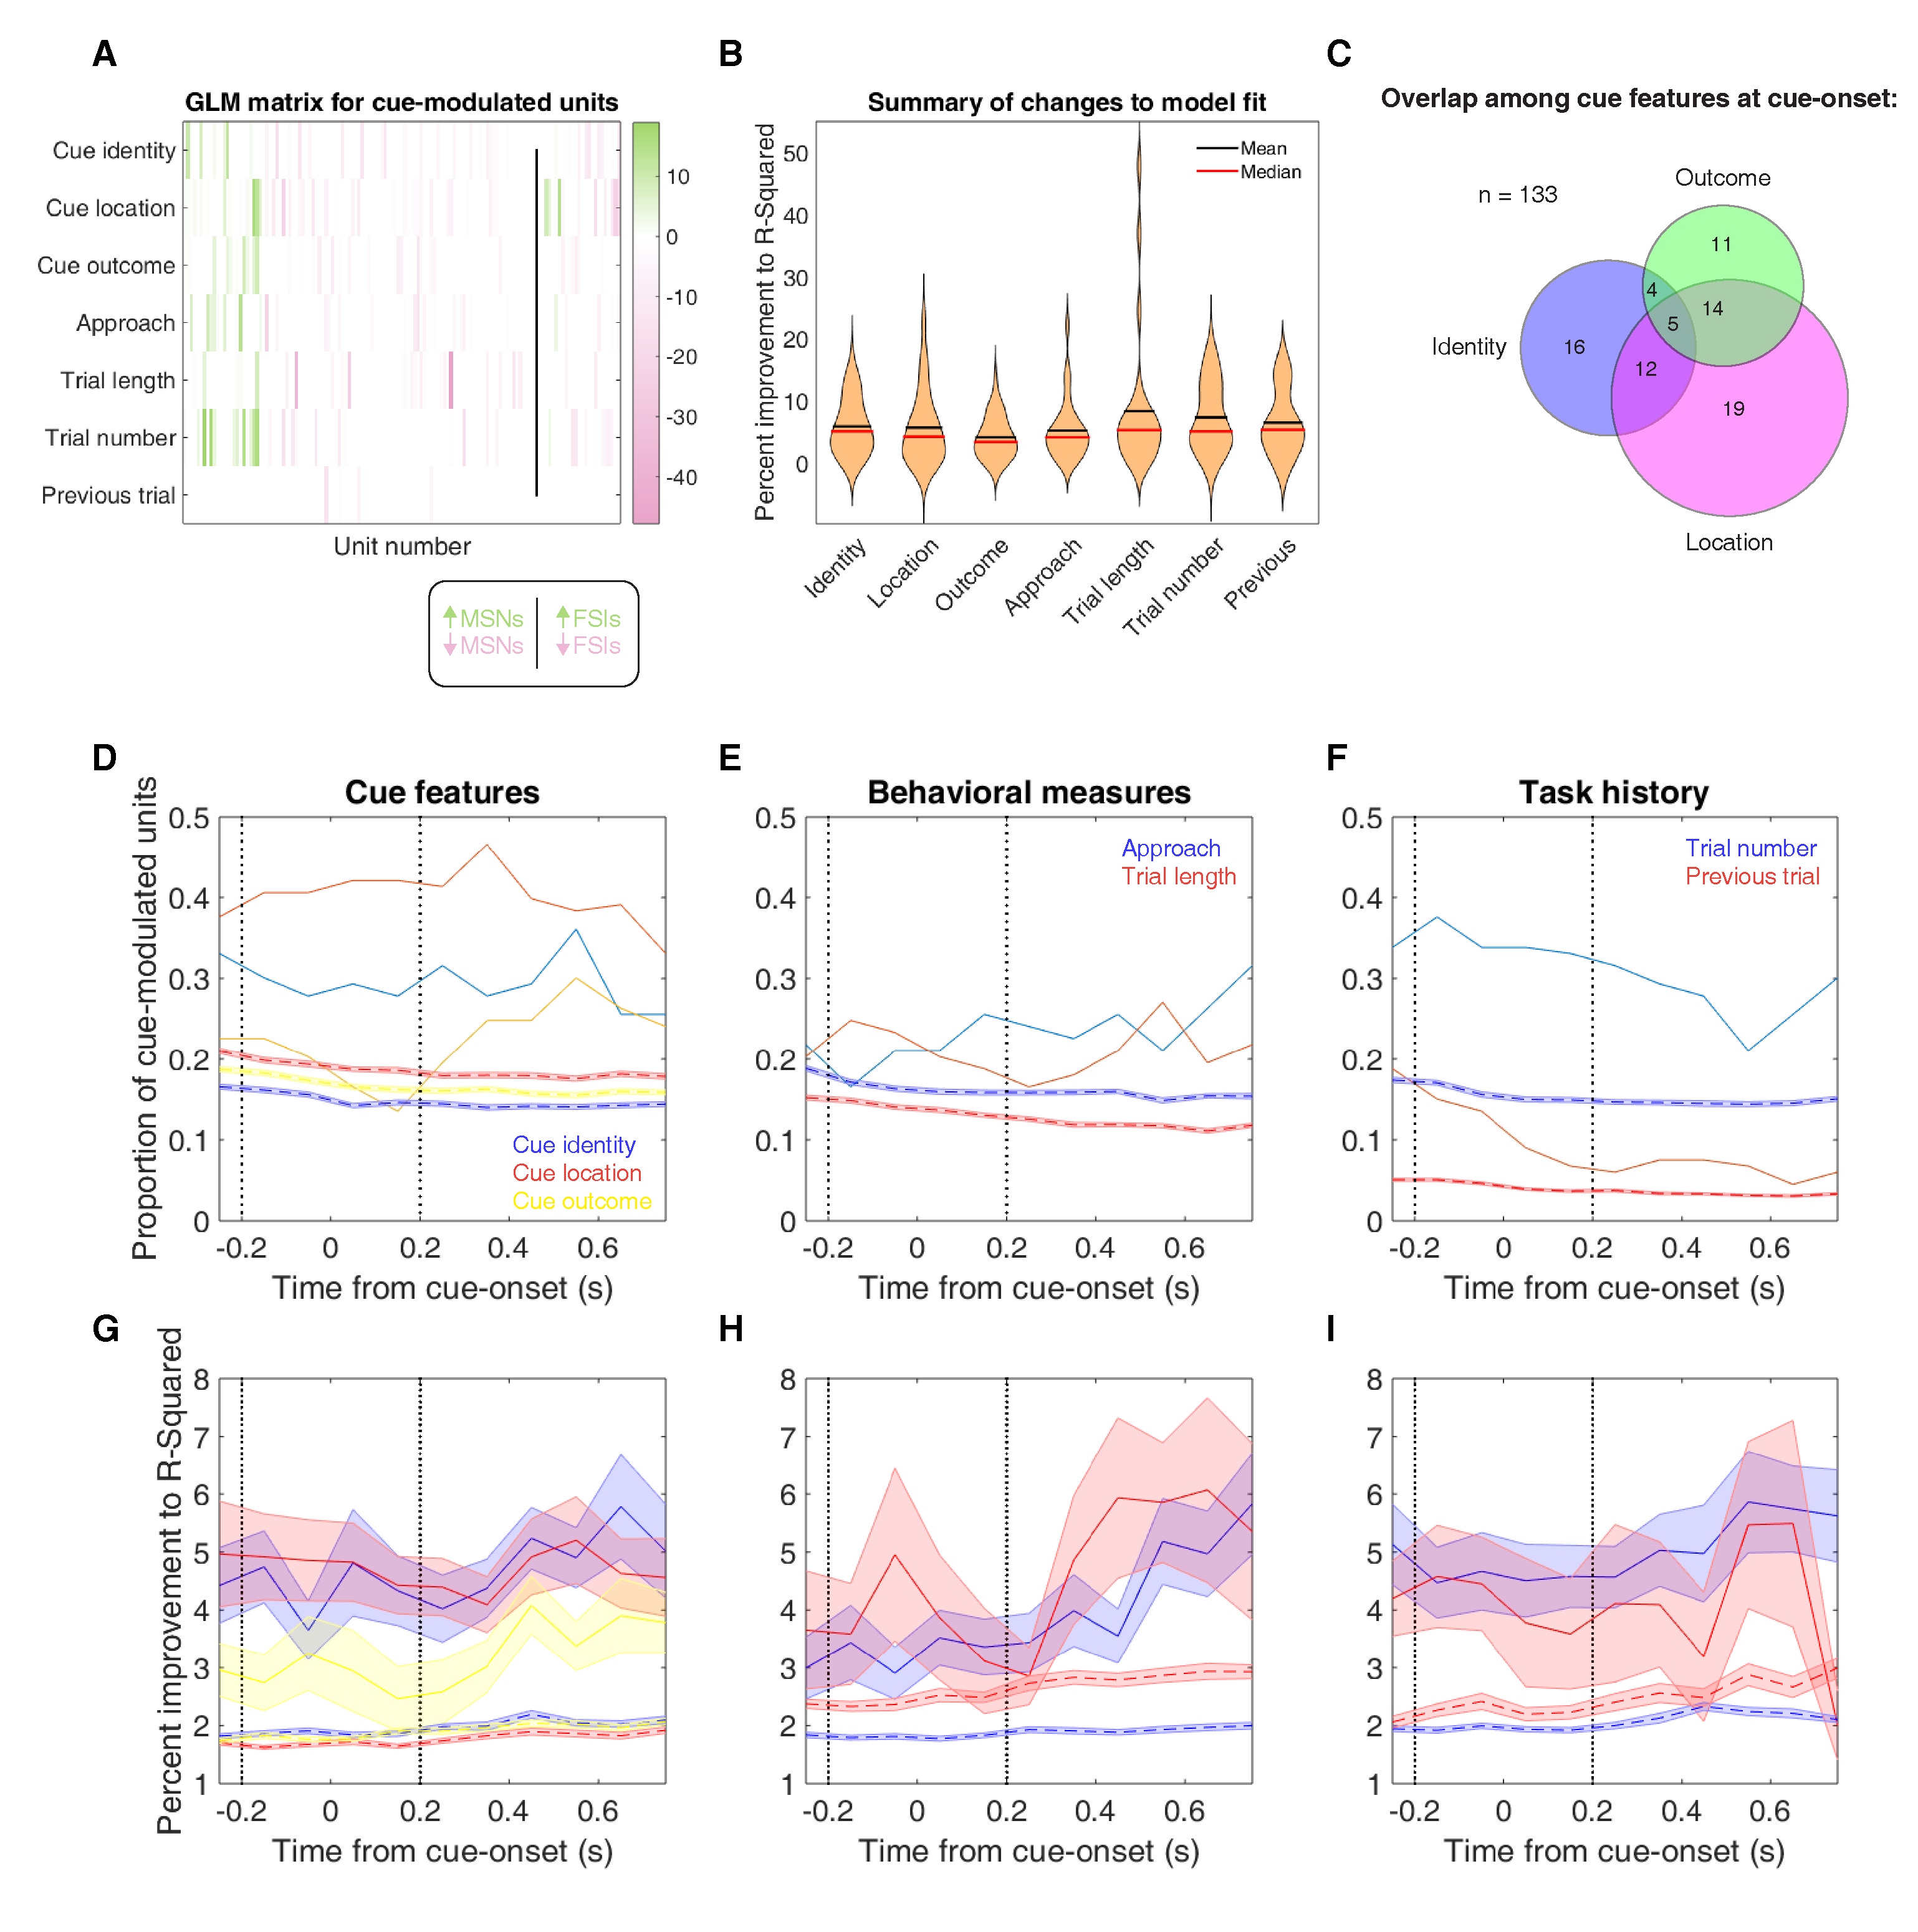
\includegraphics[width=\textwidth]{Fig 6 - GLM.png}
\caption{Summary of influence of various task parameters on cue-modulated NAc
  units after cue-onset. \DIFdelbeginFL \DIFdelFL{A. }\DIFdelendFL \DIFaddbeginFL \DIFaddFL{\bsf{A}: }\DIFaddendFL GLM matrix \DIFdelbeginFL \DIFdelFL{demonstrating impact }\DIFdelendFL \DIFaddbeginFL \DIFaddFL{illustrating the contribution }\DIFaddendFL of
  various task parameters \DIFdelbeginFL \DIFdelFL{on }\DIFdelendFL \DIFaddbeginFL \DIFaddFL{to }\DIFaddendFL NAc \DIFaddbeginFL \DIFaddFL{unit }\DIFaddendFL firing rates. A stepwise GLM was fit to
  each unit that showed evidence of cue modulation by a Wilcoxon signed-rank
  test. Each row represents a given task parameter, and each column \DIFdelbeginFL \DIFdelFL{is the influence of that task parameter on }\DIFdelendFL \DIFaddbeginFL \DIFaddFL{corresponds
  to }\DIFaddendFL a \DIFdelbeginFL \DIFdelFL{given }\DIFdelendFL \DIFaddbeginFL \DIFaddFL{single }\DIFaddendFL unit. \DIFdelbeginFL \DIFdelFL{Response variable is }\DIFdelendFL \DIFaddbeginFL \DIFaddFL{Colors indicate }\DIFaddendFL how much of the firing rate variance an
  individual predictor contributed to the model, as measured by differences in
  R-squared between the final model and the model minus the predictor of
  interest. Ordering from left to right: MSNs that increased firing in response
  to the cue (green, left of line), MSNs with a decreasing response (red, left
  of line), FSIs with an increasing response (green, right of line), FSIs with a
  decreasing response (red, right of line). Darker shades indicate more firing
  rate variance explained by a given predictor. Black line indicates separation
  of MSNs and FSIs. \DIFdelbeginFL \DIFdelFL{B. }\DIFdelendFL \DIFaddbeginFL \DIFaddFL{\bsf{B}: }\DIFaddendFL Violin plots demonstrating changes in R-squared
  values with the addition of each of the individual predictors. The mean,
  median, and distribution of changes in R-squared values is plotted for each of
  the seven task parameters used in the GLM.}
\label{fig:GLM}
\end{figure}
{\bf Population level averages reveal characteristic response profiles:}

\DIFdelbegin \DIFdel{A }\DIFdelend \DIFaddbegin \DIFadd{We observed a }\DIFaddend variety of single unit response profiles \DIFdelbegin \DIFdel{were observed }\DIFdelend around the time of \DIFdelbegin \DIFdel{cue-onset}\DIFdelend \DIFaddbegin \DIFadd{cue
onset (Figure \ref{fig:examples})}\DIFaddend . To investigate whether these firing rate
patterns were related to \DIFdelbegin \DIFdel{the cue information they represented, we looked at }\DIFdelend \DIFaddbegin \DIFadd{what cue features were encoded, we plotted the
}\DIFaddend population level averages for units that were modulated by each feature. To do
this\DIFaddbegin \DIFadd{, }\DIFaddend we normalized firing activity for each unit that was modulated by a given
cue feature, such as light block, then generated the cue-onset aligned
population average firing rate for each of the cue features (Figure
\ref{fig:pop}). \DIFdelbegin \DIFdel{This analyses revealed overall }\DIFdelend \DIFaddbegin \DIFadd{Overall, this analysis revealed }\DIFaddend that cells that showed an
increase upon cue presentation had stronger responses for the preferred cue
condition (Figure \ref{fig:pop}A,C,E). Interestingly, units that were classified
as decreasing in response to the cue showed a biphasic response at the
population level, with a small peak at a time in alignment with entry into the
arm, followed by a sustained dip after cue-onset (Figure
\ref{fig:pop}B,D,F). Units that were modulated by cue identity showed a stronger
increase in response to the preferred task block, as well as a higher tonic
firing rate to the preferred task block, most notably in units that decreased in
firing rate to the cue (Figure \ref{fig:pop}A,B). Units that were modulated by
cue location showed a graded response to locations of decreasing preference,
with peak firing occurring around cue-onset (Figure \ref{fig:pop}C,D). Units
that were modulated by cue outcome showed a ramping of activity after cue-onset
for their preferred cue type. Additionally, units that exhibited a decrease in
firing in response to the cue and whose activity was modulated by cue outcome,
showed a sustained discriminatory response to reward-available and
reward-unavailable cues that extended beyond cue-onset (Figure
\ref{fig:pop}F). Together, these visualizations of the averaged population
responses revealed nuanced differences in the way NAc units are modulated by cue
conditions across cue features.

\begin{figure}[h]
\centering
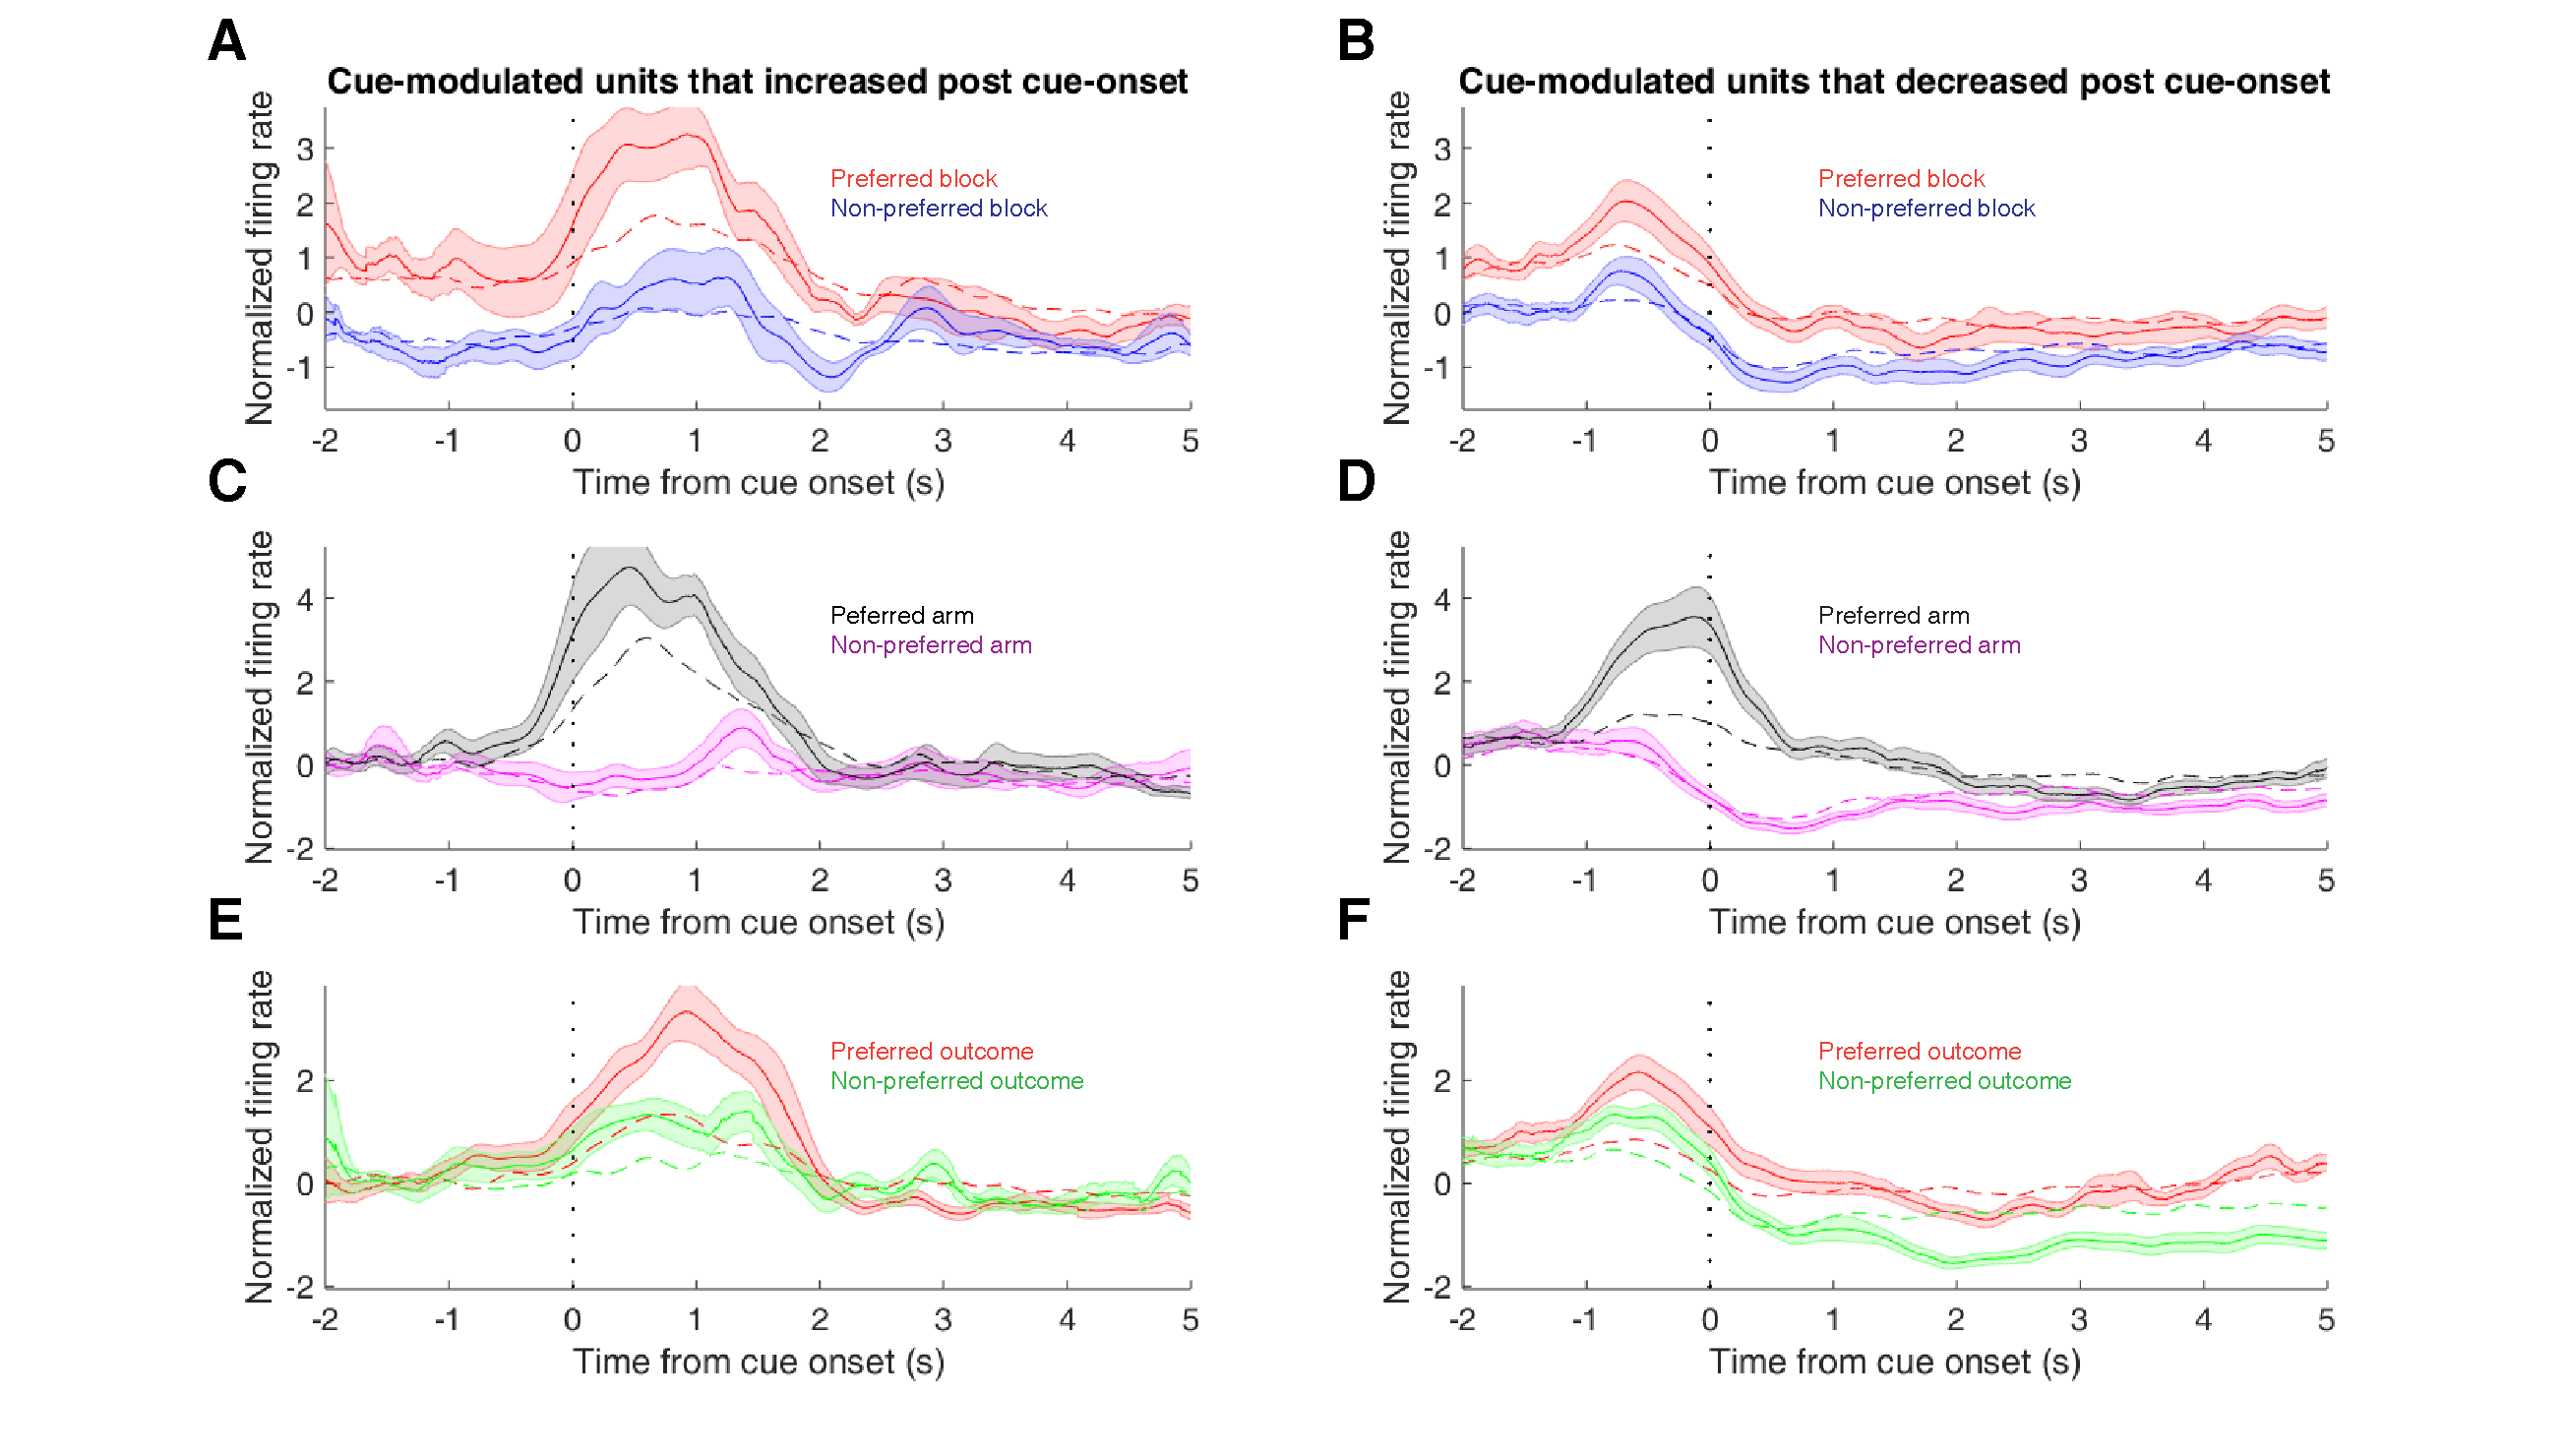
\includegraphics[width=\textwidth]{Fig 7 - Population averages.png}
\caption{Population-level averages of cue feature sensitive NAc units. \DIFdelbeginFL \DIFdelFL{A. }\DIFdelendFL \DIFaddbeginFL \DIFaddFL{\bsf{A}:
  }\DIFaddendFL Average smoothed normalized (z-score) activity for cue-modulated units where
  cue identity was a significant predictor in the GLM, aligned to
  cue-onset. Activity is plotted for preferred stimulus block (red) and
  nonpreferred stimulus block (blue). Dashed line indicates onset of
  cue. Lightly shaded area indicates standard error of the mean. Note larger
  increase to preferred stimulus block to nonpreferred stimulus block. Black
  lines indicate the average of 1000 rounds of random sampling of units from the
  non-drifting population for the preferred and non-preferred blocks. \DIFdelbeginFL \DIFdelFL{B. }\DIFdelendFL \DIFaddbeginFL \DIFaddFL{\bsf{B}:
  }\DIFaddendFL Same as A but for units that decreased in firing. Note population level
  activity reveals cells classified as “decreasing” in response to cue show a
  biphasic response at the population level, with a transient increase around
  the time the rat starts on the arm, followed by a minimum after cue
  onset. Also, note the sustained difference in firing between the two
  blocks. \DIFdelbeginFL \DIFdelFL{C-D. }\DIFdelendFL \DIFaddbeginFL \DIFaddFL{\bsf{C-D}: }\DIFaddendFL Same as A-B for cue location. Activity is plotted from most
  preferred arm (yellow), in decreasing order to least preferred arm (black,
  navy blue, magneta, respectively). Note the graded response to arms of
  decreasing preference. \DIFdelbeginFL \DIFdelFL{E-F. }\DIFdelendFL \DIFaddbeginFL \DIFaddFL{\bsf{E-F}: }\DIFaddendFL Same as A-B for cue outcome. Activity is
  plotted for preferred expected outcome (red), and nonpreferred outcome
  (green). Note the larger increase to the cue representing the cell’s preferred
  outcome (E), and the sustained decrease to the nonpreferred outcome (F).}
\label{fig:pop}
\end{figure}
{\bf NAc units dynamically segment the task:}

Given the varied time courses and response profiles of NAc units to various
aspects of the cue, the NAc may be computing a temporally evolving state value
signal (Pennartz., 2011). If this is the case, then the recruitment of NAc units
should vary alongside changes in the environment. To look at the distribution of
responses throughout our task space and see if this distribution is modulated by
cue features, we z-scored the firing rate of each unit and plotted the
normalized firing rates of all units aligned to cue-onset and sorted them
according to the time of peak firing rate (Figure \ref{fig:tiling}). We did this
separately for both the light and sound blocks, and found a nearly uniform
distribution of firing fields in task space that was not limited to alignment to
the cue (Figure \ref{fig:tiling}A). Furthermore, to determine if this population
level activity was similar across blocks, we also organized firing during the
sound blocks according to the ordering derived from the light
blocks. \DIFaddbegin {\color{red}\DIFadd{(JIMMIE EDIT THIS SECTION!)}} \DIFaddend This revealed that while there
was some preservation of order, the overall firing was qualitatively different
across the two blocks. To control for the possibility that any comparison of
trials would produce this effect, we did a within block comparison, comparing
half of the trials in the light block against the other half. This comparison
looked similar to our test comparison of sound block trials ordered by light
block trials. Additionally, given that the majority of our units showed an
inhibitory response to the cue, we also plotted the firing rates according to
the lowest time in firing, and again found some maintenance of order, but
largely different ordering across the two blocks, and the within block
comparison (Figure \ref{fig:tiling}B). To further test this, we divided each
block into two halves and looked at the correlation of the average smoothed
firing rates across various combinations of these halves across our cue-aligned
centered epoch\DIFdelbegin \DIFdel{(Table \ref{tbl3})}\DIFdelend . A linear mixed effects model revealed that within block
correlations (e.g. one half of light trials vs other half of light trials) were
higher and more similar than across block correlations (e.g. half of light
trials vs half of sound trials), suggesting that activity in the NAc
discriminates across various cue conditions \DIFaddbegin \DIFadd{(within block correlations = .381,
across block correlations = .342)}\DIFaddend . This process was repeated for cue location
and cue outcome, showing that NAc segmentation of the task is qualitatively
different even during those parts of the task not immediately associated with a
specific cue, action, or outcome, although the within condition comparison of
reward-unavailable trials was less correlated than reward-available trials, and
more similar to the across condition comparisons (Figure \ref{fig:tiling}C-F).

\begin{figure}
[h]
\centering
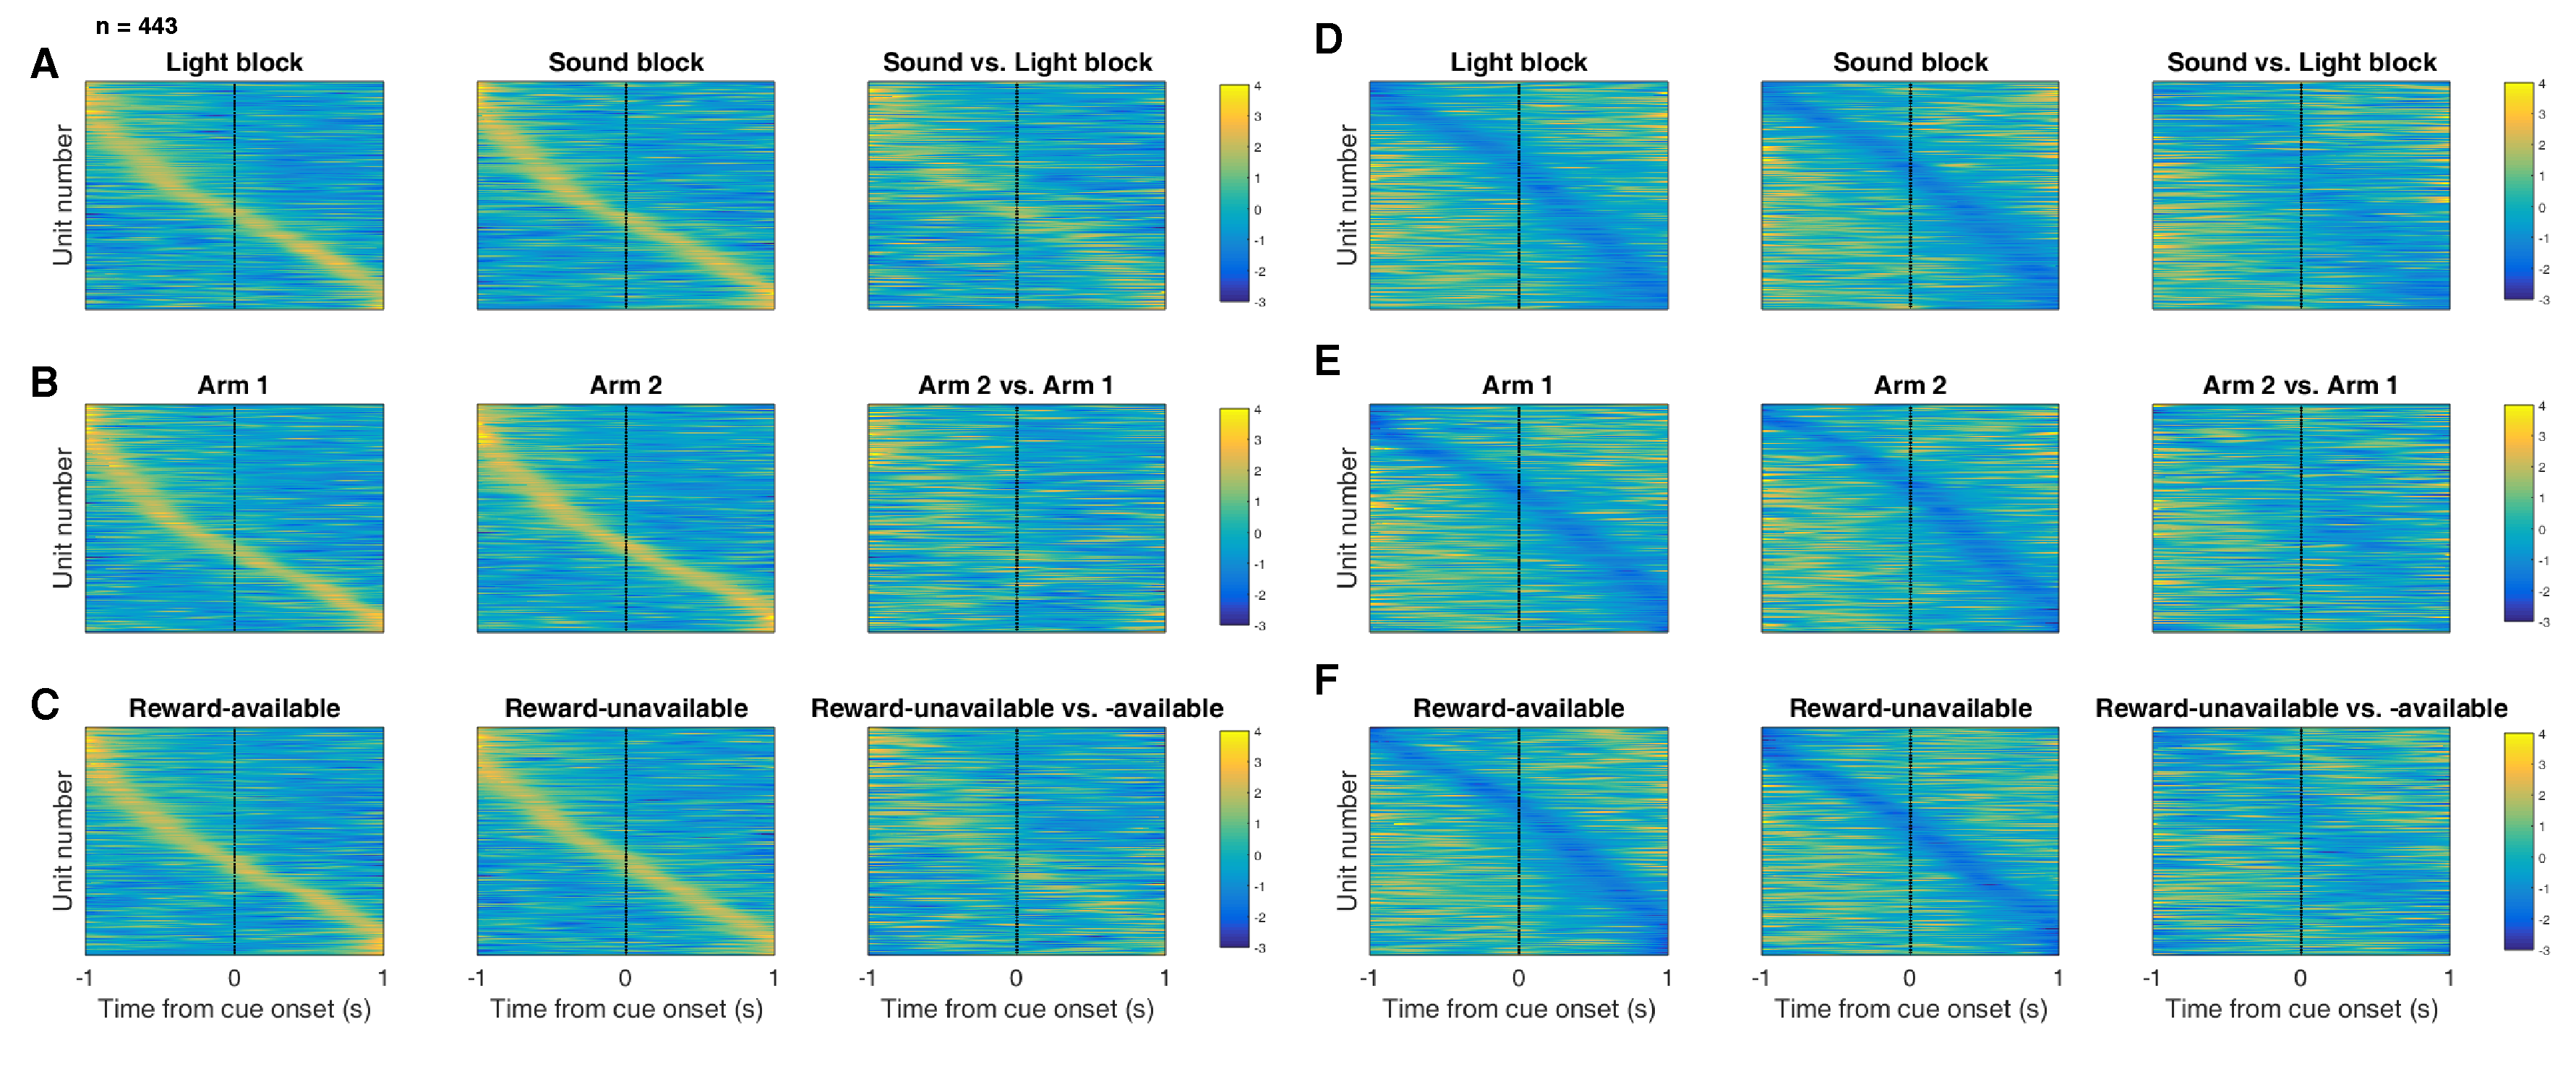
\includegraphics[height=0.5\textheight]{Fig 8 - Task tiling.png}
\caption{Distribution of NAc firing rates across time surrounding cue
  onset. Each panel shows normalized (z-score) firing rates for all recorded NAc
  units (each row corresponds to one unit) as a function of time (time 0
  indicates cue onset), averaged across all trials for a specific cue type,
  indicated by text labels. \DIFdelbeginFL \DIFdelFL{A-C. }\DIFdelendFL \DIFaddbeginFL \DIFaddFL{\bsf{A-C}: }\DIFaddendFL Heat plots aligned to normalized peak
  firing rates. A, far left: Heat plot showing smoothed normalized firing
  activity of all recorded NAc units ordered according to the time of their peak
  firing rate during the light block. Each row is a unit’s average activity
  across time to the light block. Dashed line indicates cue onset. Notice the
  yellow band across time, indicating all aspects of visualized task space were
  captured by the peak firing rates of various units. A, middle left: Same units
  ordered according to the time of the peak firing rate during the sound
  block. Note that for both blocks, units tile time approximately uniformly with
  a clear diagonal of elevated firing rates. A, middle right: Unit firing rates
  taken from the sound block, ordered according to peak firing rate taken from
  the light block. Note that a weaker but still discernible diagonal persists,
  indicating partial similarity between firing rates in the two blocks. A, far
  right: Unit firing rates taken from half of the light block, ordered according
  to peak firing rate taken from the other half of light trials. Note similar
  pattern to middle right suggests that reordering any two sets of trials
  produces this partial similarity, however correlations within blocks are more
  similar than correlations across blocks (see text). \DIFdelbeginFL \DIFdelFL{B. }\DIFdelendFL \DIFaddbeginFL \DIFaddFL{\bsf{B}: }\DIFaddendFL Same layout as in
  A, except that the panels now compare two different locations on the track
  instead of two cue modalities. As for the different cue modalities, NAc units
  clearly discriminate between locations, but also maintain some similarity
  across locations, as evident from the visible diagonal in the right panel. Two
  example locations were used for display purposes; other location pairs showed
  a similar pattern. \DIFdelbeginFL \DIFdelFL{C. }\DIFdelendFL \DIFaddbeginFL \DIFaddFL{\bsf{C}: }\DIFaddendFL Same layout as in A, except that panels now
  compare reward-available and reward-unavailable trials. D-F. Heat plots
  aligned to normalized minimum firing rates. \DIFdelbeginFL \DIFdelFL{D. }\DIFdelendFL \DIFaddbeginFL \DIFaddFL{\bsf{D}: }\DIFaddendFL Responses during
  different stimulus blocks as in A, but with units ordered according to the
  time of their minimum firing rate. \DIFdelbeginFL \DIFdelFL{E. }\DIFdelendFL \DIFaddbeginFL \DIFaddFL{\bsf{E}: }\DIFaddendFL Responses during trials on
  different arms as in B, but with units ordered by their minimum firing
  rate. \DIFdelbeginFL \DIFdelFL{F. }\DIFdelendFL \DIFaddbeginFL \DIFaddFL{\bsf{F}: }\DIFaddendFL Responses during cues signalling different outcomes as in C,
  but with units ordered by their minimum firing rate. Overall, NAc units
  "tiled" experience on the task, as opposed to being confined to specific task
  events only. Units from all sessions and animals were pooled for this
  analysis.}
\label{fig:tiling}

\end{figure}
\DIFdelbegin %DIFDELCMD < \begin{table}[p]
%DIFDELCMD < \centering
%DIFDELCMD < \setlength{\tabcolsep}{1 em} %%%
%DIF <  for the horizontal padding
%DIFDELCMD < \begin{tabular}{l c  c c c c c}
%DIFDELCMD < 

%DIFDELCMD < %%%
\DIFdelFL{Task parameter                                 }%DIFDELCMD < & %%%
\DIFdelFL{Within condition 1        }%DIFDELCMD < &%%%
\DIFdelFL{Within condition 2        }%DIFDELCMD < & %%%
\DIFdelFL{Across conditions 1        }%DIFDELCMD < &%%%
\DIFdelFL{Across conditions 2       }%DIFDELCMD < &%%%
\DIFdelFL{Across conditions 3       }%DIFDELCMD < &%%%
\DIFdelFL{Across conditions 4}%DIFDELCMD < \\
%DIFDELCMD < \hline
%DIFDELCMD < %%%
\DIFdelFL{Cue identity       }%DIFDELCMD < & %%%
\DIFdelFL{.383         }%DIFDELCMD < &%%%
\DIFdelFL{.379          }%DIFDELCMD < & %%%
\DIFdelFL{.343          }%DIFDELCMD < & %%%
\DIFdelFL{.338          }%DIFDELCMD < &%%%
\DIFdelFL{.337        }%DIFDELCMD < &%%%
\DIFdelFL{.348}%DIFDELCMD < \\
%DIFDELCMD < \hline
%DIFDELCMD < %%%
\DIFdelFL{Cue location       }%DIFDELCMD < & %%%
\DIFdelFL{.369         }%DIFDELCMD < &%%%
\DIFdelFL{.350          }%DIFDELCMD < & %%%
\DIFdelFL{.290          }%DIFDELCMD < & %%%
\DIFdelFL{.286          }%DIFDELCMD < & %%%
\DIFdelFL{.285        }%DIFDELCMD < &%%%
\DIFdelFL{.291}%DIFDELCMD < \\
%DIFDELCMD < \hline
%DIFDELCMD < %%%
\DIFdelFL{Cue outcome       }%DIFDELCMD < & %%%
\DIFdelFL{.429        }%DIFDELCMD < &%%%
\DIFdelFL{.261          }%DIFDELCMD < & %%%
\DIFdelFL{.258        }%DIFDELCMD < & %%%
\DIFdelFL{.253          }%DIFDELCMD < & %%%
\DIFdelFL{.255        }%DIFDELCMD < &%%%
\DIFdelFL{.249}%DIFDELCMD < \\
%DIFDELCMD < \hline
%DIFDELCMD < 

%DIFDELCMD < \end{tabular}
%DIFDELCMD < \caption %%%
\DIFdelendFL {\DIFdelbeginFL \DIFdelFL{Firing rate correlations}%DIFDELCMD < } %DIFDELCMD < \label{tbl3} %%%
%DIFDELCMD < \end{table}
%DIFDELCMD < 

%DIFDELCMD < {%%%
\DIFdelend \bf Encoding of cue features is maintained until outcome:}

In order to be useful for \DIFaddbegin \DIFadd{credit assignment in }\DIFaddend reinforcement learning, a trace
of the cue must be maintained until the outcome\DIFdelbegin \DIFdel{to link the
outcome to }\DIFdelend \DIFaddbegin \DIFadd{, so that information about the
outcome can be associated with }\DIFaddend the outcome-predictive cue. To test whether
representations of cue features were maintained post-approach until the outcome
was revealed, we fit a GLM to the post-approach firing rates of cue-modulated
units aligned to the time of nosepoke into the reward receptacle. This analysis
showed that a variety of units still discriminated firing according to various
cue features, but not other task parameters, showing that NAc activity
discriminates various cue conditions well into a trial (Table \ref{tbl1},
Figures \ref{fig:NP_examples},\ref{fig:NP_GLM}). Additionally, these units were
a mix between \DIFdelbegin \DIFdel{those }\DIFdelend \DIFaddbegin \DIFadd{most of the units }\DIFaddend that encoded cue features at cue-onset \DIFaddbegin \DIFadd{(observed
overlap greater than expected by chance according to chi-square tets)}\DIFaddend , and those
that did not previously have a cue feature as a predictor (29, 48, and 30 units
encoded both time points for cue identity, location, and outcome,
respectively). Fitting a GLM to all recorded units revealed a similar pattern
(data not shown). Population level averages for units that increased to
cue-onset showed a ramping up of activity that peaked upon nosepoke, whereas
units that decreased to cue-onset showed a gradual reduction of firing activity
that reached a minimum upon nosepoke (Figure \ref{fig:NP_pop}). Additionally, a
peak is seen for preferred cue outcome in decreasing units at 1 second post
cue-onset when reward was received, demonstrating an integration of expected and
received reward (Figure \ref{fig:NP_pop}F). Furthermore, aligning normalized
peak firing rates to nosepoke onset, revealed a clustering of responses around
reward receipt for all cue conditions where the rat would have received reward
(Figure \ref{fig:NP_tiling}). To determine whether coding of cue features was
maintained after the outcome was revealed, a GLM was fit to the firing rates of
cue-modulated units at the time of reward receipt, during which the cue was
still present. Fitting a GLM revealed 10 units (8\%) where cue outcome accounted
for an average of 32\% of firing rate variance (Table \ref{tbl1}, data not
shown). However, an absence of cue identity or cue location coding was observed,
suggesting that the NAc does not maintain a representation of these cue features
once the rat receives behavioral feedback for its decision.

\begin{figure}[h]
\centering
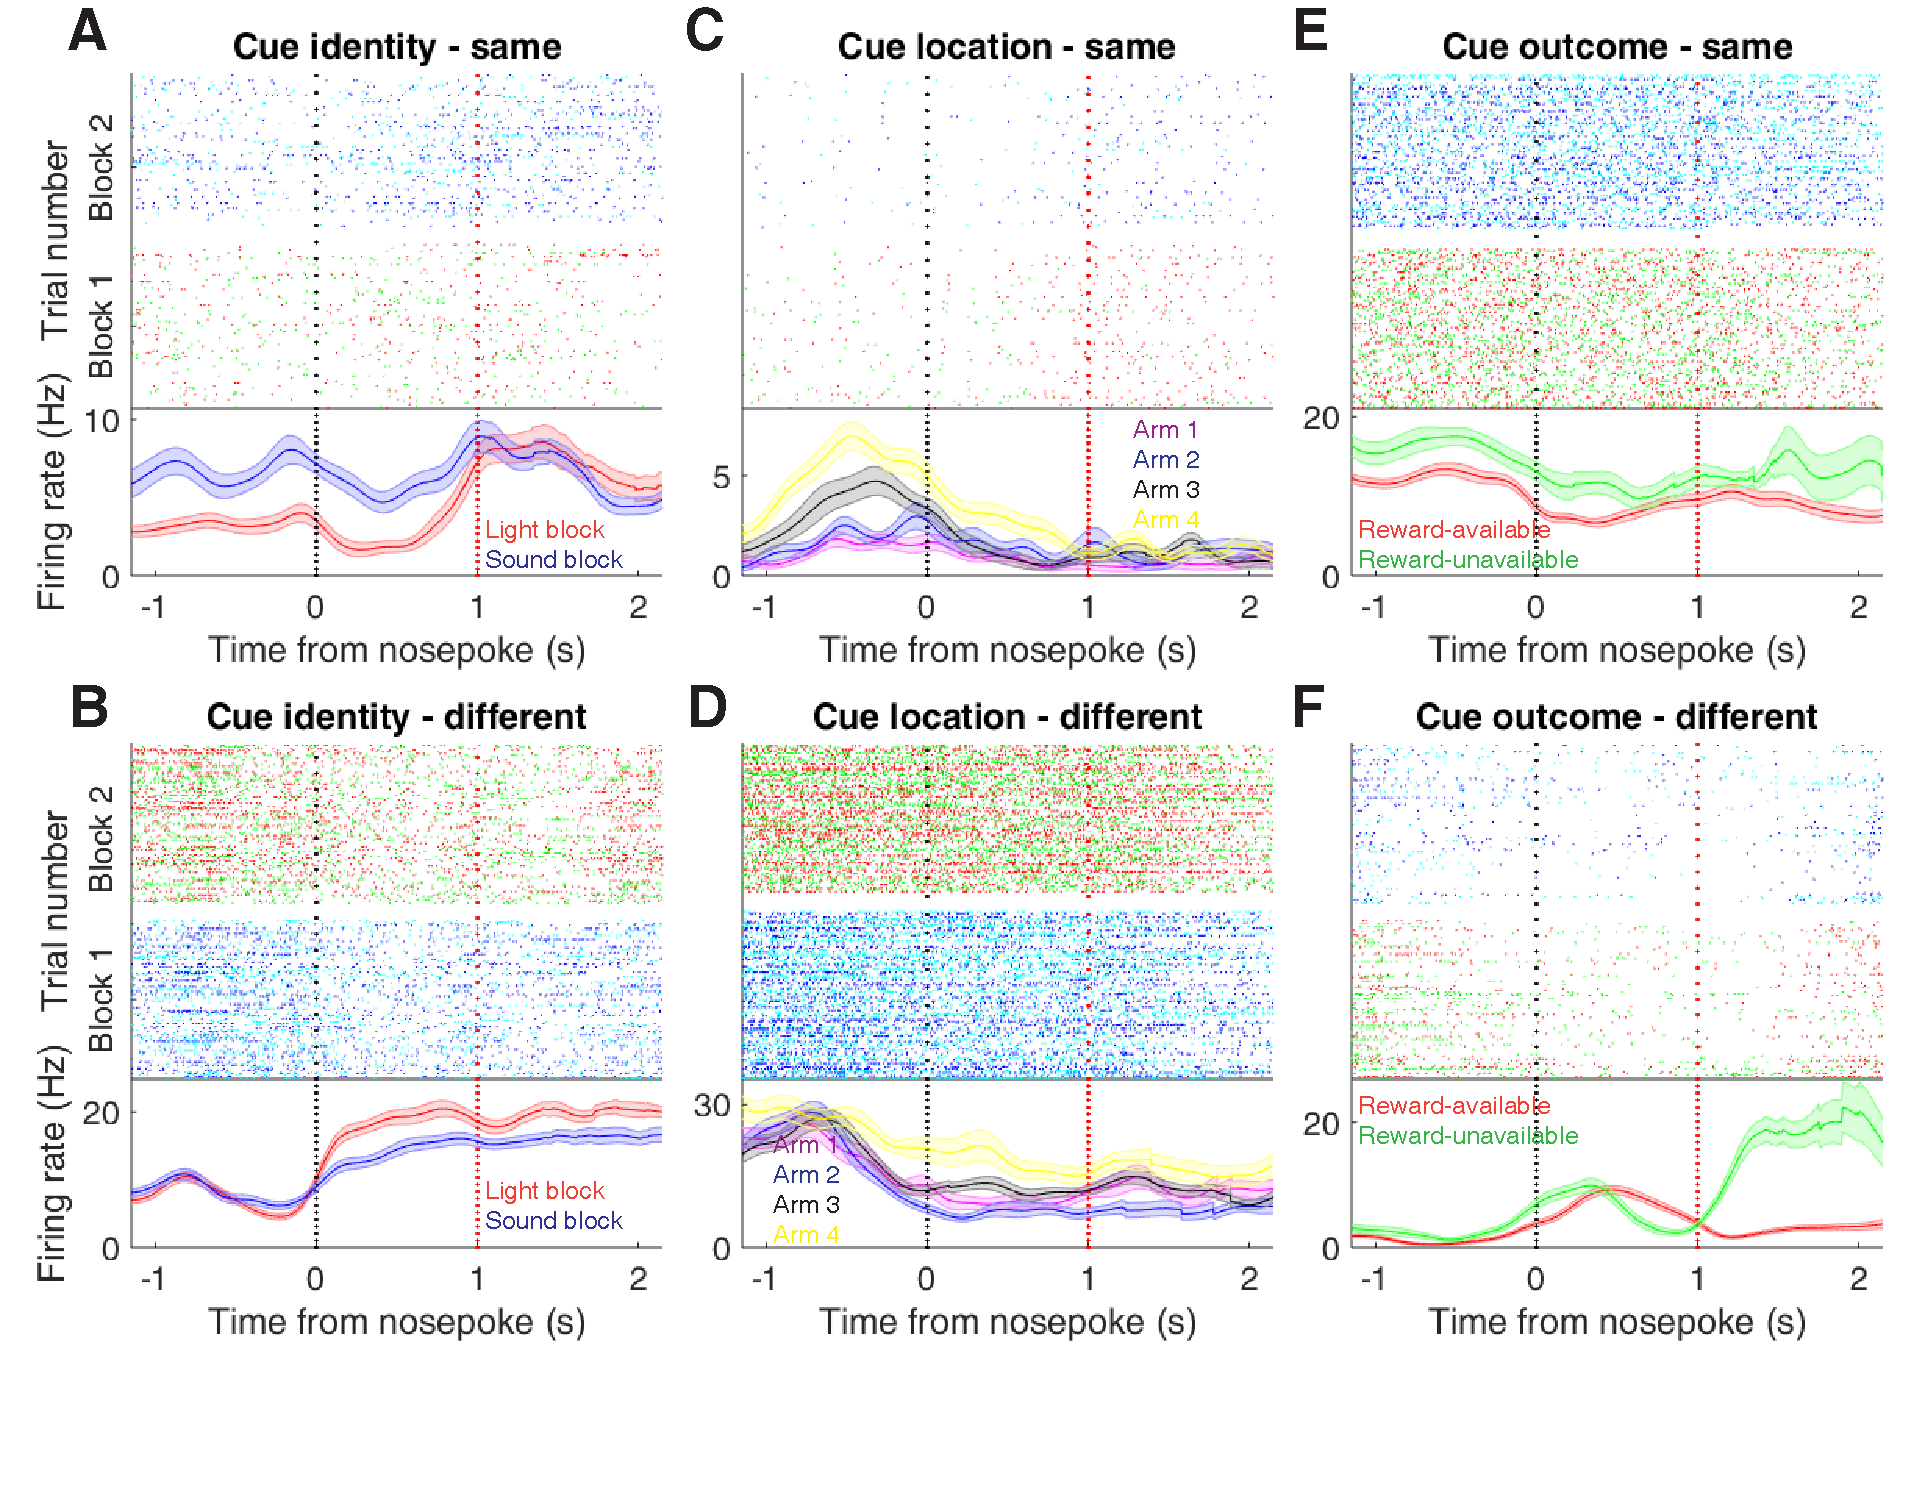
\includegraphics[width=\textwidth]{Fig 9 - NP Neural examples.png}
\caption{Examples of cue-modulated NAc units influenced by various task
  parameters at time of nosepoke. \DIFdelbeginFL \DIFdelFL{A. }\DIFdelendFL \DIFaddbeginFL \DIFaddFL{\bsf{A}: }\DIFaddendFL Example of a cue-modulated NAc unit
  that encoded cue identity at both cue-onset and during nosepoke hold. Top:
  rasterplot showing the spiking activity across all trials aligned to
  nosepoke. Spikes across trials are color coded according to cue type (red:
  reward-available light; green: reward-unavailable light; navy blue:
  reward-available sound; light blue: reward-unavailable sound). White space
  halfway up the rasterplot indicates switching from one block to the
  next. Black dashed line indicates nosepoke. Red dashed line indicates receipt
  of outcome. Bottom: PETHs showing the average smoothed firing rate for the
  unit for trials during light (red) and sound (blue) blocks, aligned to
  nosepoke. Lightly shaded area indicates standard error of the mean. Note this
  unit showed a sustained increase to sound cues during the trial. \DIFdelbeginFL \DIFdelFL{B. }\DIFdelendFL \DIFaddbeginFL \DIFaddFL{\bsf{B}: }\DIFaddendFL An
  example of a unit that was responsive to cue identity at time of nosepoke but
  not cue-onset. \DIFdelbeginFL \DIFdelFL{C-D. }\DIFdelendFL \DIFaddbeginFL \DIFaddFL{\bsf{C-D}: }\DIFaddendFL Cue-modulated units that encoded cue location, at
  both cue-onset and nosepoke (C), and only nosepoke (D). Each color in the
  PETHs represents average firing response for a different cue
  location. \DIFdelbeginFL \DIFdelFL{E-F. }\DIFdelendFL \DIFaddbeginFL \DIFaddFL{\bsf{E-F}: }\DIFaddendFL Cue-modulated units that encoded cue outcome, at both
  cue-onset and nosepoke (E), and only nosepoke (F), with the PETHs comparing
  reward-available (red) and reward-unavailable (green) trials.}
\label{fig:NP_examples}
\end{figure}
\begin{figure}[h]
\centering
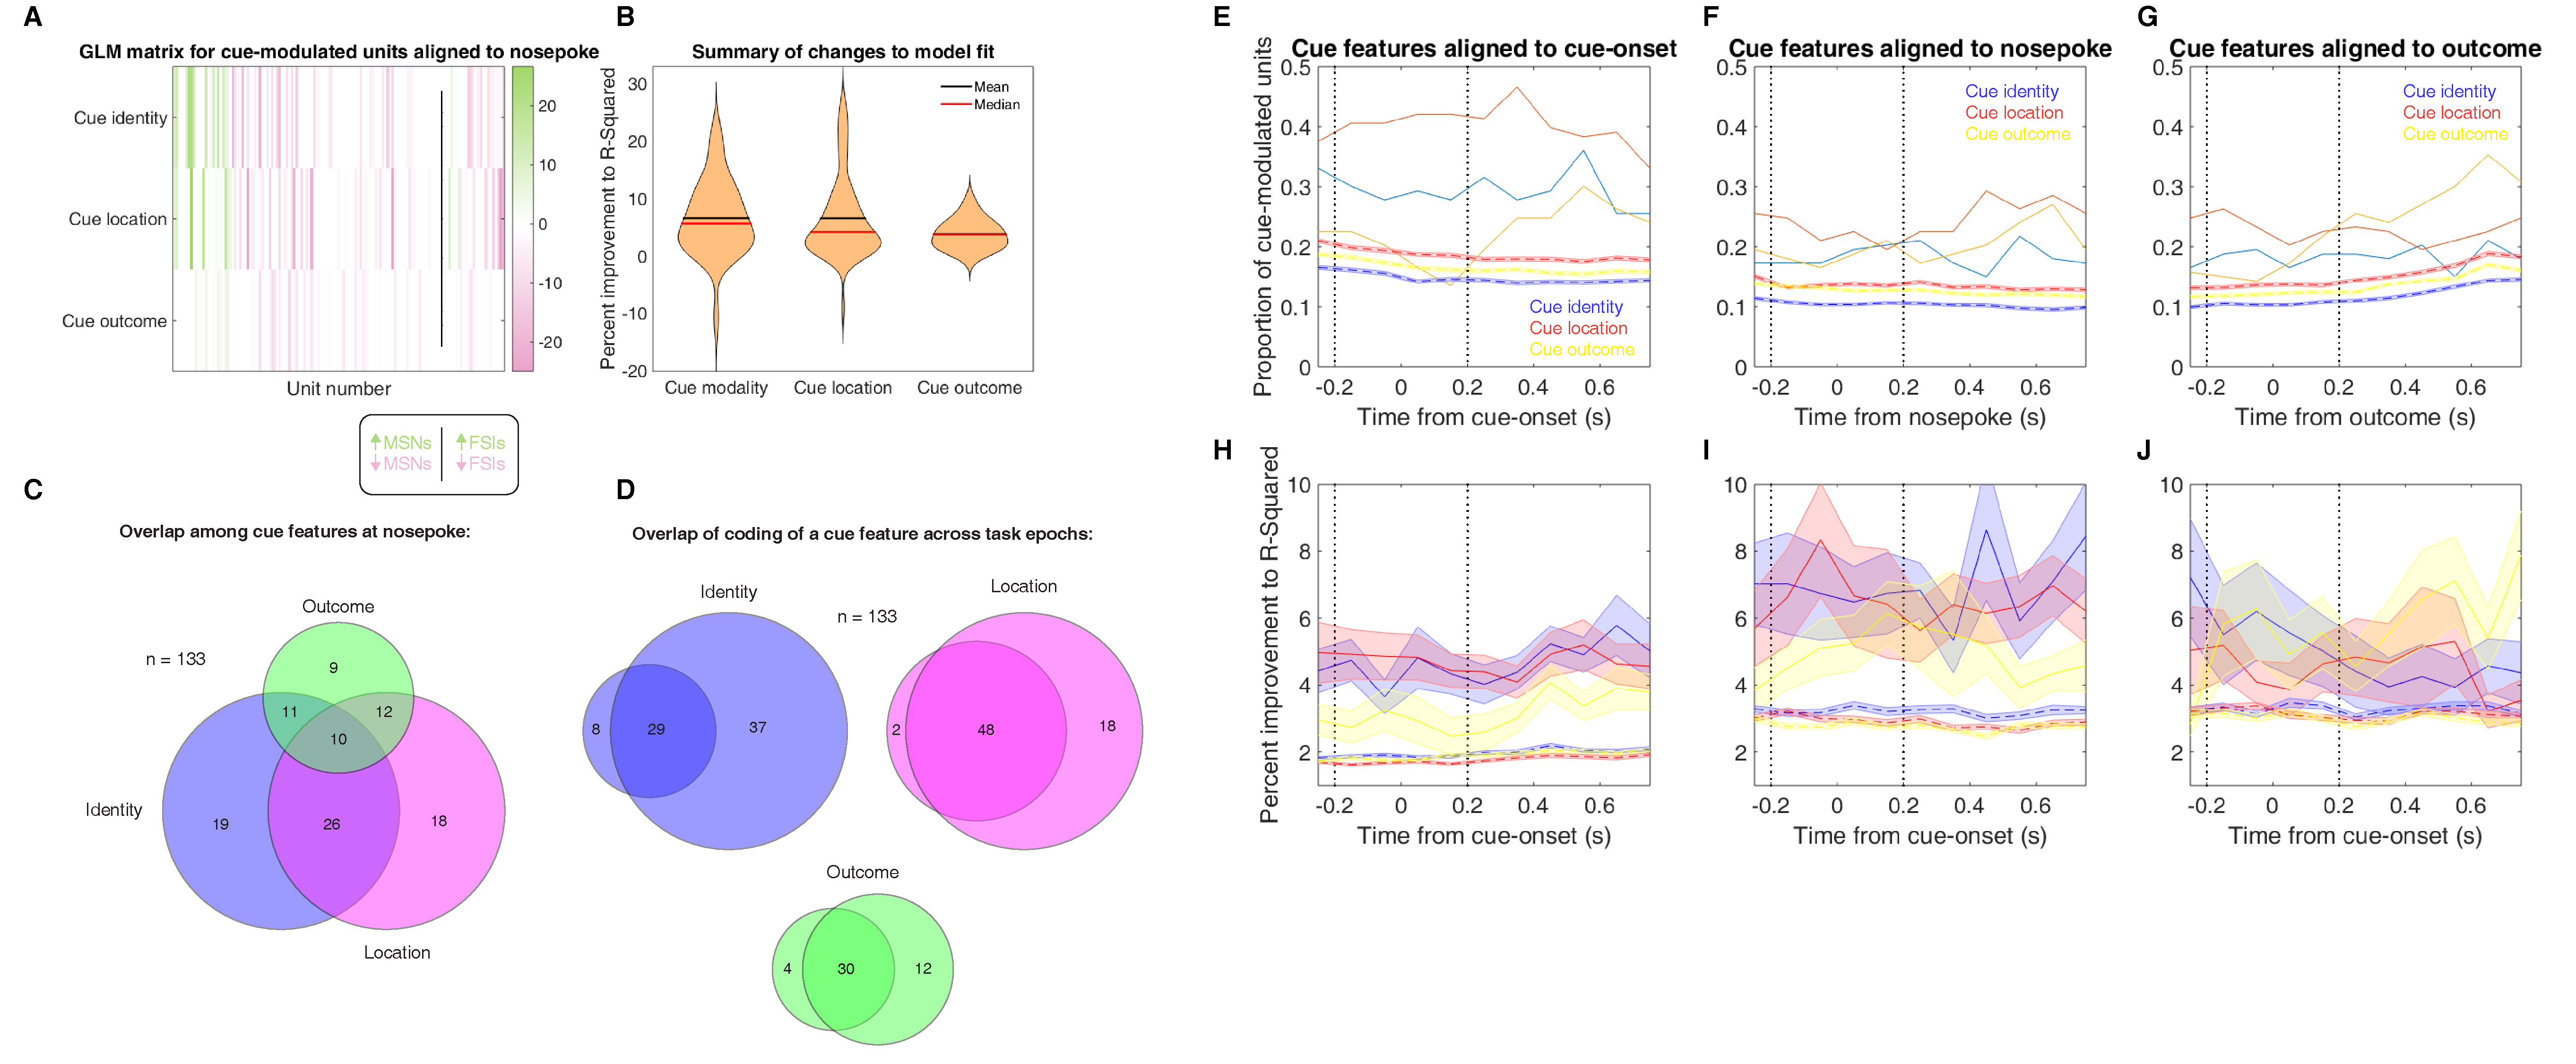
\includegraphics[width=\textwidth]{Fig 10 - NP GLM.png}
\caption{Summary of influence of various task parameters of cue-modulated NAc
  units during nosepoke. \DIFdelbeginFL \DIFdelFL{A. }\DIFdelendFL \DIFaddbeginFL \DIFaddFL{\bsf{A}: }\DIFaddendFL GLM matrix demonstrating impact of various
  task parameters on NAc firing rates. A stepwise GLM was fit to each unit that
  showed evidence of cue modulation by a Wilcoxon signed-rank test. Each row
  represents a given task parameter, and each column is the influence of that
  task parameter on a given unit. Response variable is how much of the firing
  rate variance an individual predictor contributed to the model, as measured by
  differences in R-squared between the final model and the model minus the
  predictor of interest. Ordering from left to right: MSNs that increased firing
  in response to the cue (green, left of line), MSNs with a decreasing response
  (red, left of line), FSIs with an increasing response (green, right of line),
  FSIs with a decreasing response (red, right of line). Darker shades indicate
  more firing rate variance explained by a given predictor. Black line indicates
  separation of MSNs and FSIs. \DIFdelbeginFL \DIFdelFL{B. }\DIFdelendFL \DIFaddbeginFL \DIFaddFL{\bsf{B}: }\DIFaddendFL Violin plots demonstrating changes in
  R-squared values with the addition of each of the individual predictors. The
  mean, median, and distribution of changes in R-squared values is plotted for
  each of the three task parameters that were significant predictors in the
  GLM.}
\label{fig:NP_GLM}
\end{figure}
\begin{figure}[h]
\centering
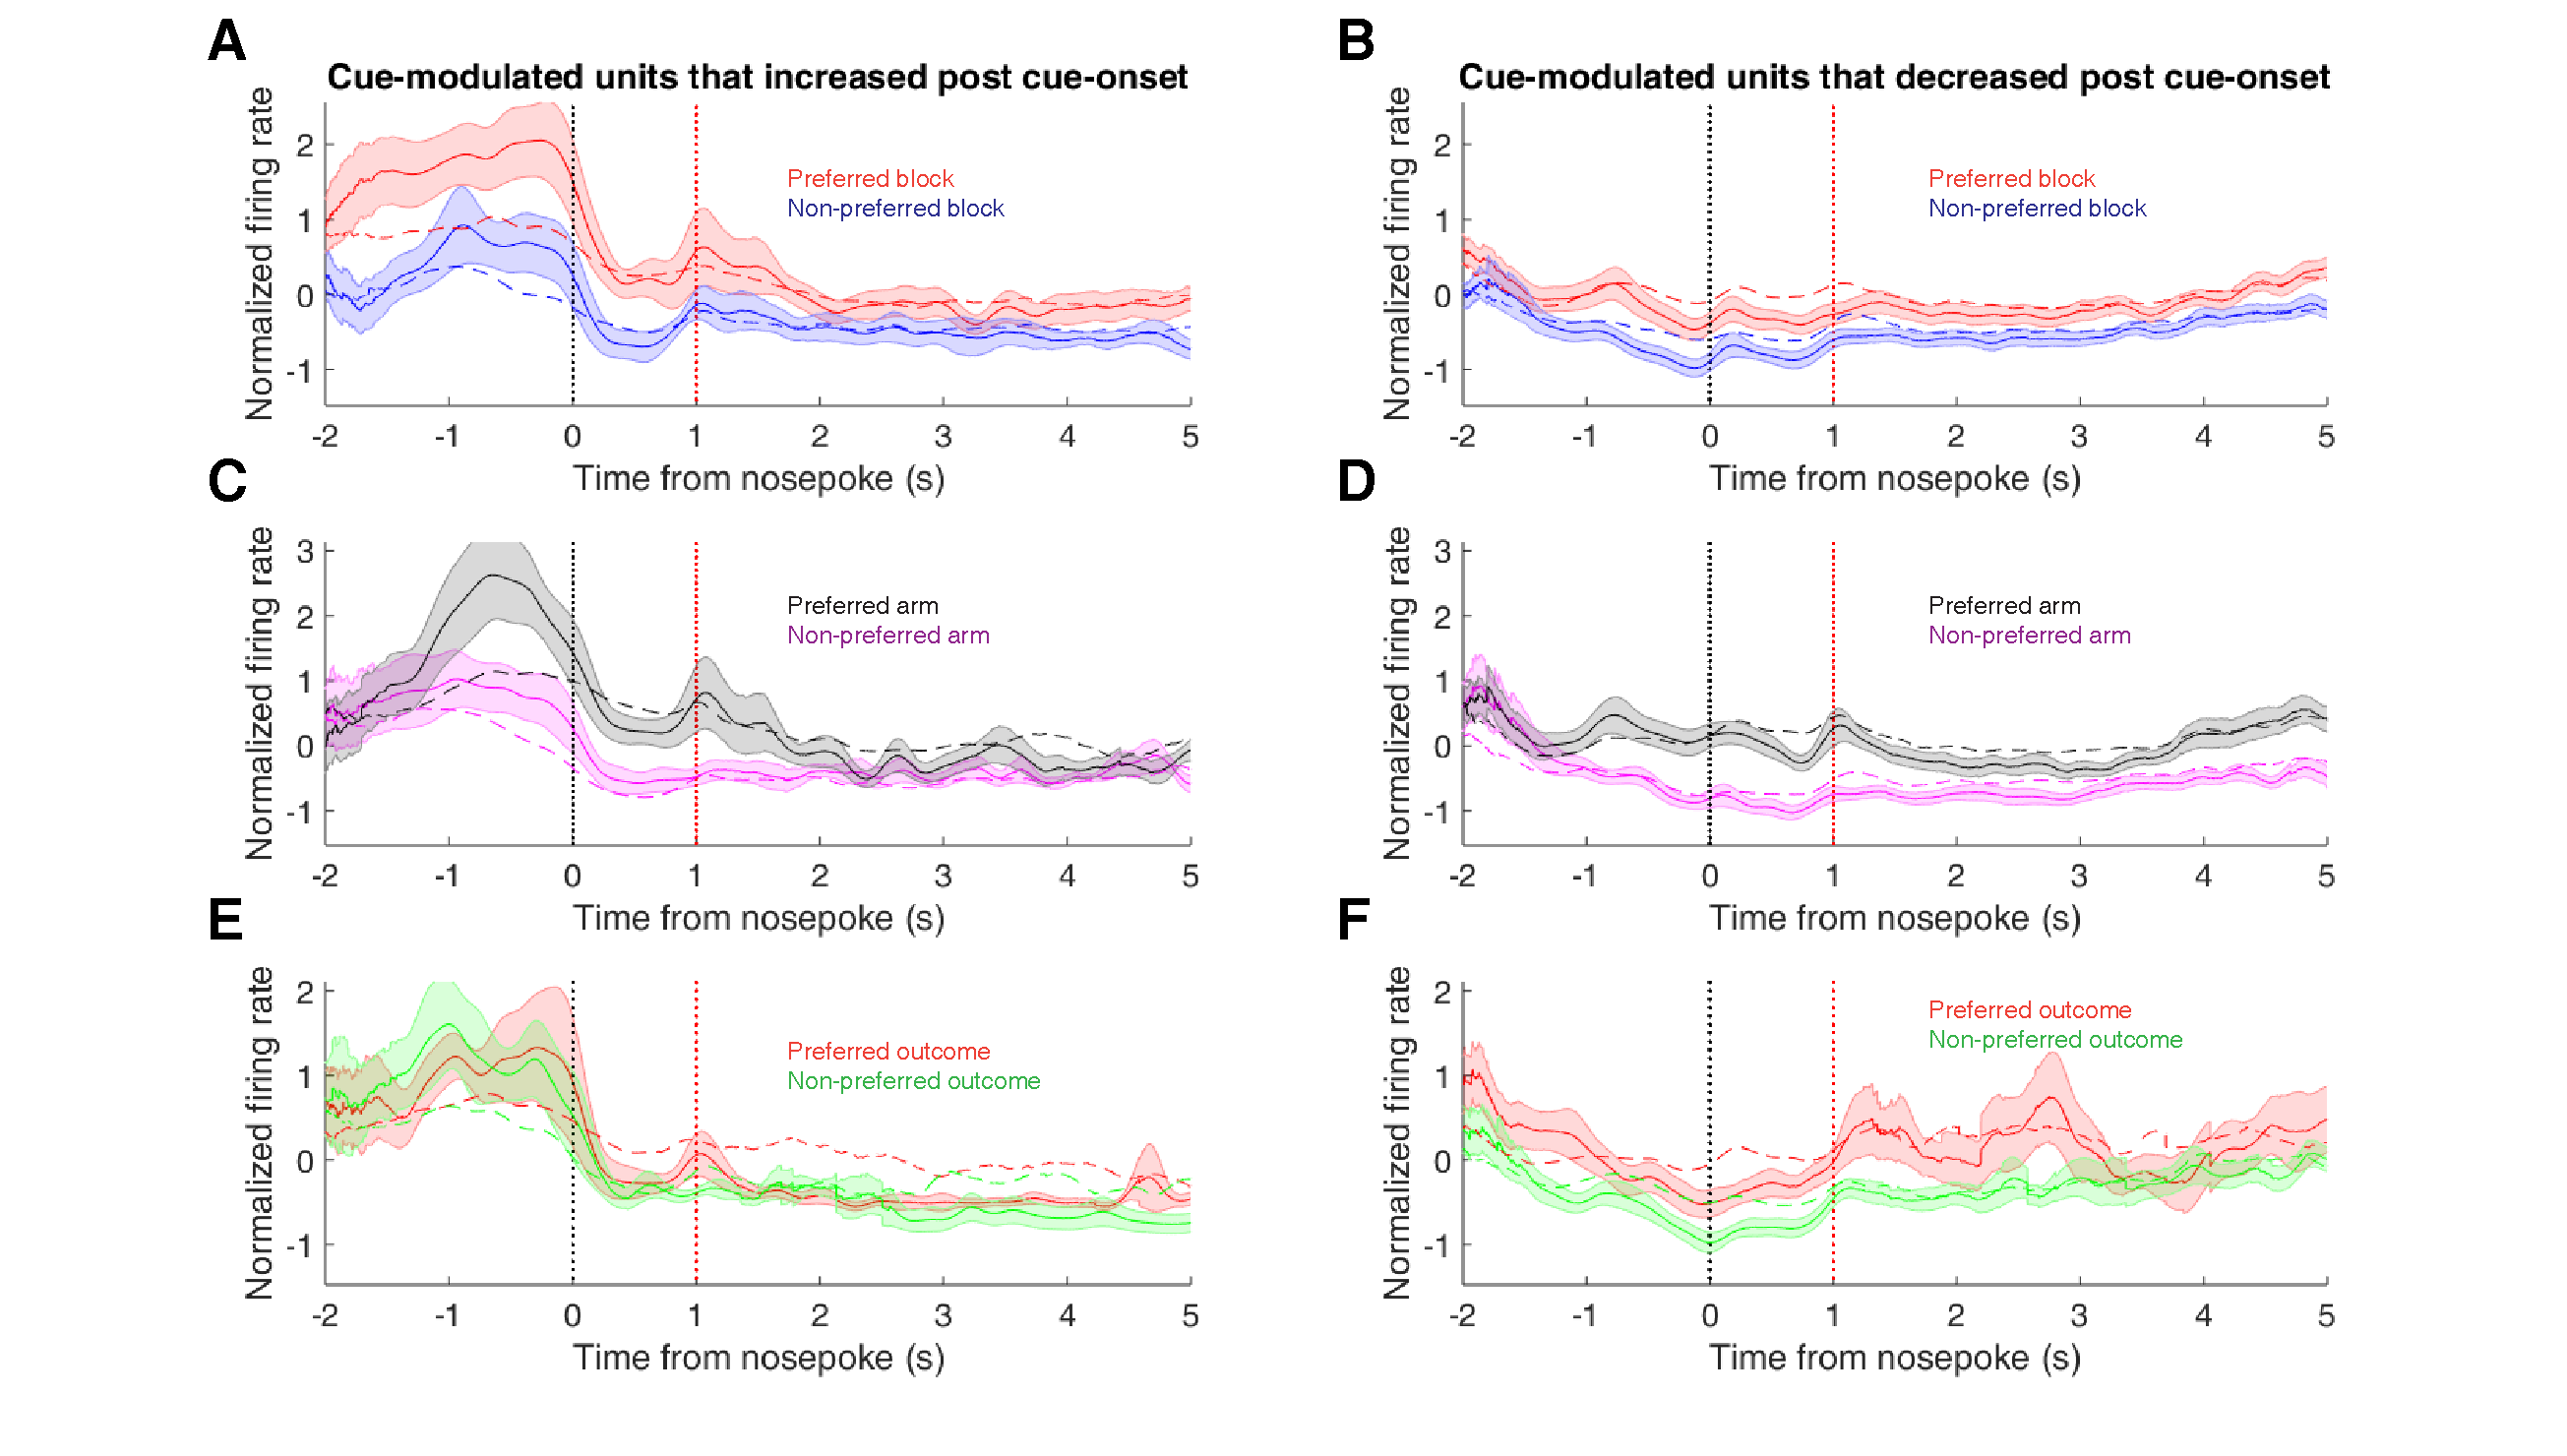
\includegraphics[width=\textwidth]{Fig 11 - NP population averages.png}
\caption{Population-level averages of cue feature sensitive NAc units during a
  nosepoke. \DIFdelbeginFL \DIFdelFL{A. }\DIFdelendFL \DIFaddbeginFL \DIFaddFL{\bsf{A}: }\DIFaddendFL Average smoothed normalized activity for cue-modulated
  units where cue identity was a significant predictor in the GLM, aligned to
  nosepoke with reward delivery occurring 1 s after nosepoke. Activity is
  plotted for preferred stimulus block (red) and nonpreferred stimulus block
  (blue). Black dashed line indicates nosepoke. Red dashed line indicates reward
  delivery occurring 1 s after nosepoke for reward-available trials. Lightly
  shaded area indicates standard error of the mean. Note larger increase leading
  up to nosepoke to preferred stimulus block to nonpreferred stimulus
  block. \DIFdelbeginFL \DIFdelFL{B. }\DIFdelendFL \DIFaddbeginFL \DIFaddFL{\bsf{B}: }\DIFaddendFL Same as A but for units that decreased in firing. Note the
  sustained difference in firing between the two blocks. \DIFdelbeginFL \DIFdelFL{C-D. }\DIFdelendFL \DIFaddbeginFL \DIFaddFL{\bsf{C-D}: }\DIFaddendFL Same as A-B
  for cue location. Activity is plotted from most preferred arm (yellow), in
  decreasing order to least preferred arm (black, navy blue, magneta,
  respectively). Note the subtle but graded response to arms of decreasing
  preference. \DIFdelbeginFL \DIFdelFL{E-F. }\DIFdelendFL \DIFaddbeginFL \DIFaddFL{\bsf{E-F}: }\DIFaddendFL Same as A-B for cue outcome. Activity is plotted for
  preferred expected outcome (red), and nonpreferred outcome (green). Note the
  peak after reward receipt for preferred outcome in decreasing cells (F).}
\label{fig:NP_pop}
\end{figure}
\begin{figure}
[h]
\centering
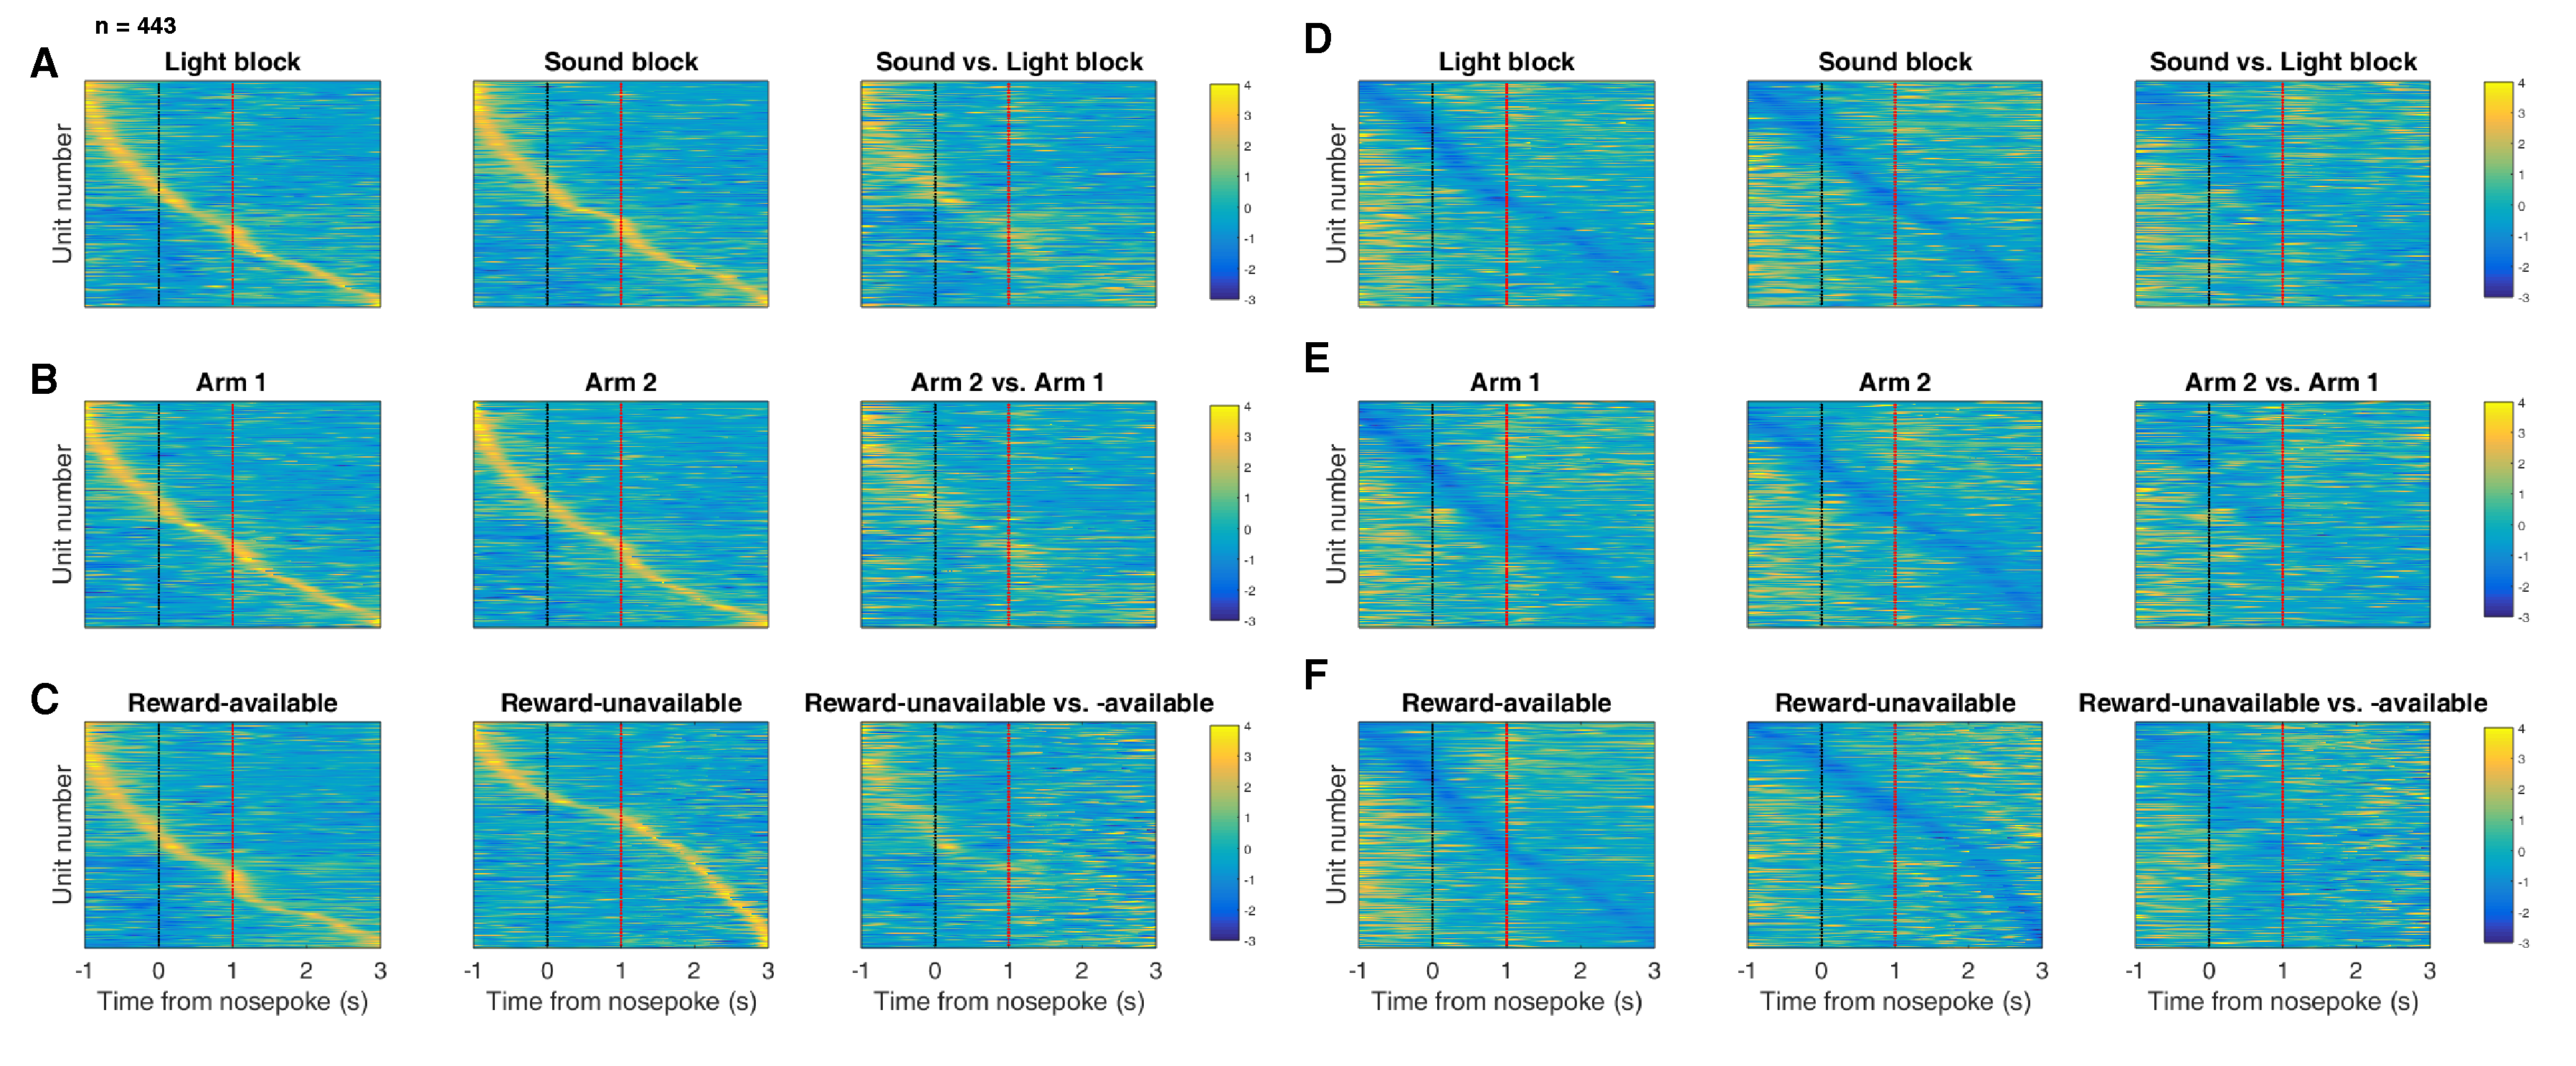
\includegraphics[height=0.5\textheight]{Fig 12 - NP task tiling.png}
\caption{Distribution of NAc firing rates across task space during approach
  trials. Each panel shows normalized firing rates for all recorded NAc units
  (each row corresponds to one unit) as a function of time (time 0 indicates
  nosepoke), averaged across all approach trials for a specific cue type,
  indicated by text labels. \DIFdelbeginFL \DIFdelFL{A}\DIFdelendFL \DIFaddbeginFL \DIFaddFL{\bsf{A}}\DIFaddendFL , far left: Heat plot showing smoothed
  normalized firing activity of all recorded NAc units ordered according to the
  time of their peak firing rate during the light block. Each row is a unit’s
  average activity across time to the light block. Black dashed line indicates
  nosepoke. Red dashed line indicates reward delivery occurring 1 s after
  nosepoke for reward-available trials. Notice the yellow band across time,
  indicating all aspects of visualized task space were captured by the peak
  firing rates of various units. A, middle left: Same units ordered according to
  the time of the peak firing rate during the sound block. Note that for both
  blocks, units tile time approximately uniformly with a clear diagonal of
  elevated firing rates, and a clustering around reward receipt. A, middle
  right: Unit firing rates taken from the sound block, ordered according to peak
  firing rate taken from the light block. Note that a weaker but still
  discernible diagonal persists, indicating partial similarity between firing
  rates in the two blocks. A, far right: Unit firing rates taken from half of
  the light block, ordered according to peak firing rate taken from the other
  half of light trials. Note similar pattern to middle right suggests that
  reordering any two sets of trials produces this partial similarity, however
  correlations within blocks are more similar than correlations across blocks
  (see text). \DIFdelbeginFL \DIFdelFL{B}\DIFdelendFL \DIFaddbeginFL \DIFaddFL{\bsf{B}}\DIFaddendFL : Same layout as in A, but with units ordered according to
  the time of their minimum firing rate. \DIFdelbeginFL \DIFdelFL{C}\DIFdelendFL \DIFaddbeginFL \DIFaddFL{\bsf{C}}\DIFaddendFL : Same layout as in A, except
  that the panels now compare two different locations on the track instead of
  two cue modalities. As for the different cue modalities, NAc units clearly
  discriminate between locations, but also maintain some similarity across
  locations, as evident from the visible diagonal in the right panel. Two
  example locations were used for display purposes; other location pairs showed
  a similar pattern. \DIFdelbeginFL \DIFdelFL{D}\DIFdelendFL \DIFaddbeginFL \DIFaddFL{\bsf{D}}\DIFaddendFL : As for C, but with units ordered by their minimum
  firing rate. \DIFdelbeginFL \DIFdelFL{E}\DIFdelendFL \DIFaddbeginFL \DIFaddFL{\bsf{E}}\DIFaddendFL : Same layout as in A, except that panels now compare
  reward-available and reward-unavailable trials. Notice the absence of a
  cluster of tiling around reward receipt for reward-unavailable
  trials. \DIFdelbeginFL \DIFdelFL{F}\DIFdelendFL \DIFaddbeginFL \DIFaddFL{\bsf{F}}\DIFaddendFL : As for A, but with units ordered by their minimum firing
  rate. Overall, NAc units "tiled" experience on the task, as opposed to being
  confined to specific task events only. Units from all sessions and animals
  were pooled for this analysis.}
\label{fig:NP_tiling}

\end{figure}
\section*{Discussion}

The present study found evidence for coding\DIFdelbegin \DIFdel{of }\DIFdelend \DIFaddbegin \DIFadd{, by partially overlapping populations of NAc units, of }\DIFaddend multiple identifying features of motivationally relevant stimuli in addition to expected outcome; the sensory modality of the presented cue, as well at its physical location \DIFdelbegin \DIFdel{within the track , and that this }\DIFdelend \DIFaddbegin \DIFadd{on the track (H2 and H3 in Figure \ref{fig:schematic}A). Importantly, this identity }\DIFaddend coding was maintained on approach trials during a delay period where the rat held a nosepoke until receipt of outcome \DIFdelbegin \DIFdel{. Furthermore, this coding was both independent, and intermixed across cue features and behavioral measures. Coding at the population level revealed qualitatively distinct comparison profiles across cue features, such as cells that encoded cue modality tended to sustain the discriminatory firing outside of cue presentation, while a subset cells that discriminated reward-available from reward-unavailable cues maintained this discrimination until after reward receipt. Across }\DIFdelend \DIFaddbegin \DIFadd{(H2 in Figure \ref{fig:schematic}B). Cells that coded different cue features exhibited different temporal profiles as a whole, although across }\DIFaddend all recorded cells \DIFdelbegin \DIFdel{, }\DIFdelend a tiling of task structure was observed such that all points within our analyzed task space was accounted for by the ordered peak firing rates of all cells\DIFdelbegin \DIFdel{, and }\DIFdelend \DIFaddbegin \DIFadd{. Furthermore, }\DIFaddend this tiling differed between various conditions with a cue feature, such as light versus sound blocks. 
\DIFdelbegin \DIFdel{Cells that }\DIFdelend \DIFaddbegin 

{\bf \DIFadd{Cue identity:}}

\DIFadd{Our finding that NAc units can discriminate between outcome-predictive stimuli with similar biological significance, in the current study cues from different sensory modalities, expands upon an extensive rodent literature examining NAc correlates of conditioned stimuli \mbox{%DIFAUXCMD
\cite{Atallah2014,Bissonette2013,Cooch2015,Day2006,Dejean2017,Goldstein2012,Lansink2012,McGinty2013,Nicola2004,Roesch2009a,Roitman2005,Saddoris2011,Setlow2003,Sugam2014,West2016}}\hspace{0pt}%DIFAUXCMD
. Units that }\DIFaddend discriminated across blocks were not simply due to drifting of the signal across trials, as \DIFdelbegin \DIFdel{cells }\DIFdelend \DIFaddbegin \DIFadd{units }\DIFaddend that showed a drift in firing between the first and second half within a block were excluded from the analysis. Furthermore, even though actions were stereotyped during correct trials, such that the rat always turned left at the decision point to approach for reward, and right to skip the receptacle and initiate the next trial, \DIFdelbegin \DIFdel{cells }\DIFdelend \DIFaddbegin \DIFadd{units }\DIFaddend that were modulated by the expected value of the cue maintained their specific firing patterns even during error trials where the rat turned left after presentation of the reward-unavailable cue, suggesting that these signals did not represent action values. Additionally, NAc signals have been shown to be modulated by response vigor, to detangle this from our results we included the trial length as a predictor in our GLMs, and found \DIFdelbegin \DIFdel{cells with }\DIFdelend \DIFaddbegin \DIFadd{units with cue feature }\DIFaddend correlates independent of trial length \DIFdelbegin \DIFdel{.
}%DIFDELCMD < 

%DIFDELCMD < {\bf %%%
\DIFdel{Potential functional consequences of maintained coding:}%DIFDELCMD < }
%DIFDELCMD < 

%DIFDELCMD < %%%
\DIFdel{NAc has been shown to encode stimulus-outcome associations. In reinforcement learning, these associations are commonly framed as a value estimate tied to the reward-predicting stimulus. This view, while informative, may not be complete in the sense that these value estimates may be more complex than just an agnostic value signal, for instance, the NAc is tuned to the identity of a reward. Our goal was to expand our understanding of the informational content of these outcome-predictive signals to include aspects of this environmental signal expected to be encoded by the NAc based on it’s corticolimbic inputs (discrete cues - amygdala input, spatial context - hpc input, task rules/set, behavioral strategy - pfc input). Having an enriched (multidimensional?) representation that includes details about the environmental context the animal finds itself and is maintained online until the outcome is revealed could be useful for assigning credit of a reward to the appropriate elements of an environment, to develop an accurate value function and optimize long term acquisition of reward (2012 Lee - eligibility trace). From a motivated behavior standpoint, the presence of these enriched representations can help inform action selection involving Pavlovian behaviors (conditioned approach), and after a decision has been made the maintained representation can help to hold the response in the face of competing alternatives while waiting for an outcome (Floresco 2015 summarizes this literature). 
}%DIFDELCMD < 

%DIFDELCMD < %%%
\DIFdel{If these representations function as an eligibility trace, then there should be a relationship between the content and robustness of these representations and the degree to which organisms form adaptive associations between reinforcers and their environment, which could contribute to the presence of prediction errors in the NAc in those that learned an experimental task in humans versus those that did not (Schonberg 2007). In the present experiment, understanding what information about the environment the NAc is keeping track of when reward arrives could be useful for potentially determining what representations are being reinforced. Would be interesting to see if selectively reward an animal when certain representations are active (e.g. arm 1), would help shape their assignment of reward to that arm. Could be useful for altering a maladaptive preference back to a more adaptive one, as the loss of certain aspects of coding via BLA and PFC inputs leads to the loss of outcome-predictive activity to discrete cues in the NAc. Furthermore, non-discriminatory coding in the NAc could hypothetically be correlated to over-generalization of situations, in which the animal may not recognize it is in a different situation and perform actions that are inefficient or maladaptive for reward procurement.  
}%DIFDELCMD < 

%DIFDELCMD < {\bf %%%
\DIFdel{Cue identity:}%DIFDELCMD < }
%DIFDELCMD < 

%DIFDELCMD < %%%
\DIFdel{Our finding that NAc units can discriminate between outcome-predictive stimuli with similar biological significance, in the current study cues from different sensory modalities, expands upon an extensive literature examining neural correlates of conditioned stimuli. }\DIFdelend \DIFaddbegin \DIFadd{\mbox{%DIFAUXCMD
\cite{McGinty2013}}\hspace{0pt}%DIFAUXCMD
. }\DIFaddend Perhaps the most comparable work in rodents comes from a study that found distinct coding for an odor when it predicted separate but equally valued rewards \DIFdelbegin \DIFdel{(Cooch)}\DIFdelend \DIFaddbegin \DIFadd{\mbox{%DIFAUXCMD
\cite{Cooch2015}}\hspace{0pt}%DIFAUXCMD
}\DIFaddend . The present work is complementary to this as it shows that NAc \DIFdelbegin \DIFdel{cells }\DIFdelend \DIFaddbegin \DIFadd{units }\DIFaddend have representations of identifiable aspects of the cue itself, \DIFdelbegin \DIFdel{in addition to }\DIFdelend \DIFaddbegin \DIFadd{both separately and integrated with }\DIFaddend the reward it predicts \DIFaddbegin \DIFadd{(H2 and H3 in Figure \ref{fig:schematic}A)}\DIFaddend . Another study paired separate cues with appetitive or aversive outcomes, and found separate populations of \DIFdelbegin \DIFdel{cells that encode }\DIFdelend \DIFaddbegin \DIFadd{units that encoded }\DIFaddend each cue, with many switching selectivity after reversal of the associations between the cues and outcomes, providing evidence that the NAc encodes the biological significance of stimuli \DIFaddbegin \DIFadd{\mbox{%DIFAUXCMD
\cite{Setlow2003}}\hspace{0pt}%DIFAUXCMD
}\DIFaddend . Once again, our study was different as we recorded neural responses to distinct cues encoding the same anticipated outcome, suggesting that even when the biological relevance of these stimuli is similar \DIFdelbegin \DIFdel{, }\DIFdelend the NAc dissociates their representations at the level of the single-unit\DIFdelbegin \DIFdel{(Setlow)}\DIFdelend , although this doesn’t explain the difference in population averaged firing rate for the epochs when the cue is not present. \DIFaddbegin \DIFadd{A possible interpretation of this coding of cue features alongside expected outcome is that these representations are used to associate reward with relevant features of the environment, so-called credit assignment in the reinforcement learning literature \mbox{%DIFAUXCMD
\cite{sutton1998}}\hspace{0pt}%DIFAUXCMD
. A burgeoning body of human and non-human primate work has started to elucidated neural correlates of credit assignment in the PFC, particularly in the lateral orbitofrontal cortex \mbox{%DIFAUXCMD
\cite{Akaishi2016,Asaad2017,Chau2015,Noonan2017}}\hspace{0pt}%DIFAUXCMD
. Given the importance of cortical inputs in NAc associative representations, it is possible that information related to credit assignment is relayed from the cortex to NAc \mbox{%DIFAUXCMD
\cite{Cooch2015,Ishikawa2008}}\hspace{0pt}%DIFAUXCMD
. 
}

\DIFaddend Another possibility is that these modality specific \DIFdelbegin \DIFdel{cells }\DIFdelend \DIFaddbegin \DIFadd{units }\DIFaddend were encoding the context, rule, or sequence within a session as some \DIFdelbegin \DIFdel{cells responded similar }\DIFdelend \DIFaddbegin \DIFadd{units responded similarly }\DIFaddend for both reward-available and reward-unavailable cues within a block. This interpretation is in alignment with a recent paper from the non-human primate literature that recorded NAc responses during the Wisconsin Card Sorting Task (WCST), a common set-shifting task used in both the laboratory and clinic, and found \DIFdelbegin \DIFdel{cells }\DIFdelend \DIFaddbegin \DIFadd{units }\DIFaddend that preferred firing to stimuli when a certain rule, or rule category was currently active \DIFdelbegin \DIFdel{(Sleezer)}\DIFdelend \DIFaddbegin \DIFadd{\mbox{%DIFAUXCMD
\cite{Sleezer2016}}\hspace{0pt}%DIFAUXCMD
}\DIFaddend . Indeed, an encoding of the current strategy could be an explanation as to why a sustained difference in population averaged firing was seen across stimulus blocks, as well as a potential explanation for the differentially tiling of task structure across blocks in the current study. Further support for a modulation of NAc responses by strategy comes from an fMRI study that examined BOLD levels during a set-shifting task \DIFdelbegin \DIFdel{(FitzGerald et al. , 2014). }\DIFdelend \DIFaddbegin \DIFadd{\mbox{%DIFAUXCMD
\cite{Fitzgerald2014}}\hspace{0pt}%DIFAUXCMD
. }\DIFaddend In this task, participants learned two sets of stimulus-outcome contingencies, a visual set and auditory set. During testing they were presented with both simultaneously, and the stimulus dimension that was relevant was periodically shifted between the two. Here, they found that bilateral NAc activity reflected value representations \DIFdelbegin \DIFdel{of whatever }\DIFdelend \DIFaddbegin \DIFadd{for }\DIFaddend the currently relevant stimulus dimension\DIFdelbegin \DIFdel{was}\DIFdelend , and not the irrelevant stimulus. The current finding of separate, but overlapping, populations of \DIFdelbegin \DIFdel{cells }\DIFdelend \DIFaddbegin \DIFadd{units }\DIFaddend encoding cue modality and expected value, suggests that the fMRI finding is generated by the combined activity of several different functional cell types.

A caveat of the current study is that rats were never presented with both sets of cues simultaneously, and thus never had to switch strategies, although extrapolating the data from the primate study \DIFdelbegin \DIFdel{, }\DIFdelend suggests that the activity of the cue identity \DIFdelbegin \DIFdel{cells }\DIFdelend \DIFaddbegin \DIFadd{units }\DIFaddend would be modulated by relevance. Keeping along this theme, the current data set is unable to identity precisely what the modality-sensitive neurons were encoding, that is were they tracking representations of stimulus identity, a preferred context, or even a macroscale representation of progress through the session. Furthermore, their relevance for ongoing behavior is also uncertain. NAc core lesions have been shown to impair shifting between different behavioral strategies, and it is possible that selectively silencing the \DIFdelbegin \DIFdel{cells }\DIFdelend \DIFaddbegin \DIFadd{units }\DIFaddend that prefer responding for a given modality or rule would impair performance when the animal is required to use that information, or artificial enhancement of those \DIFdelbegin \DIFdel{cells }\DIFdelend \DIFaddbegin \DIFadd{units }\DIFaddend would cause them to use the rule when it is the inappropriate strategy.

{\bf Encoding of position:}

Our finding that cue-evoked activity was modulated by cue location \DIFdelbegin \DIFdel{sides with some of the literature (Lavoie, 1994; Tabuchi, 2000; Strait, 2016). An alternative explanation for a pure spatial representation, is that these are task segmentation correlates}\DIFdelend \DIFaddbegin \DIFadd{is in alignment with several previous reports \mbox{%DIFAUXCMD
\cite{Lavoie1994,Mulder2005,Strait2016,Wiener2003}}\hspace{0pt}%DIFAUXCMD
. The NAc receives strong inputs from the hippocampus, and the communication of place-reward information across the two structures suggests that the NAc might be keeping track of locations associated with reward \mbox{%DIFAUXCMD
\cite{Lansink2008,Lansink2009,Lansink2016,Pennartz2004,Sjulson2017,Tabuchi2000,VanderMeer2011}}\hspace{0pt}%DIFAUXCMD
. Alternatively, it is possible that this positional modulation is part of a representation of task space}\DIFaddend , keeping track of where in the task the rat is. A previous non-human primate \DIFdelbegin \DIFdel{paper has shown }\DIFdelend \DIFaddbegin \DIFadd{experiment showed }\DIFaddend that when reward is contingent upon completion of a series of trials, separate populations of NAc neurons signal the start of a schedule, subsequent trials in the schedule, and the first trial in extended schedules \DIFdelbegin \DIFdel{(Shidara et al. , 1998). }\DIFdelend \DIFaddbegin \DIFadd{\mbox{%DIFAUXCMD
\cite{Shidara1998}}\hspace{0pt}%DIFAUXCMD
. }\DIFaddend This signalling of position within a sequence has been observed in subsequent studies, and it is possible that the \DIFdelbegin \DIFdel{our }\DIFdelend rats were keeping track of which specific arm they were in as part of a sequence of arms, \DIFdelbegin \DIFdel{and not just strictly a spatial representation (Mulder, 2004 and 2005; Khamassi et al. , 2008; Berke, 2009). Also, given that our task is }\DIFdelend \DIFaddbegin \DIFadd{especially since they started from the same arm during the start of each session \mbox{%DIFAUXCMD
\cite{Atallah2014,Berke2009,Khamassi2008,Lansink2012,Mulder2004}}\hspace{0pt}%DIFAUXCMD
. Given that the current task was }\DIFaddend pseudo-random, it is possible that the rats learned \DIFdelbegin \DIFdel{which cue to anticipate}\DIFdelend \DIFaddbegin \DIFadd{the structure of sequential cue presentation}\DIFaddend , and the neural activity could reflect this. However, this is unlikely as including a ‘previous trial’ variable in the analysis did not explain a significant amount of firing rate variance in response to the cue for the vast majority of cells. \DIFaddbegin \DIFadd{A limitation of the current study is that the behavioral relevance of cue location was not manipulated in the sense that varying cue location did not change the outcome-predictive nature of the cue}\DIFaddend . 

{\bf \DIFdelbegin \DIFdel{Mixed selectivity}\DIFdelend \DIFaddbegin \DIFadd{Potential functional consequences of maintained coding}\DIFaddend :}

\DIFdelbegin \DIFdel{Several other papers have reported unit profiles that integrate different task-related variables. These papers report integrated coding between expected value and subsequent motor responses, expected value and identity of a reward, and a combination of spatial-}\DIFdelend \DIFaddbegin \DIFadd{In the current study we found that the coding of cue features persisted after the choice point, during a delay period while the rat waited at the receptacle for the outcome (H2 in Figure \ref{fig:schematic}B). Having an enriched representation that includes details about the environmental context the animal finds itself in alongside expected outcome}\DIFaddend , \DIFdelbegin \DIFdel{movement-}\DIFdelend \DIFaddbegin \DIFadd{and is maintained online until the outcome is revealed could be useful for assigning credit of a reward to the appropriate elements of an environment, to develop an accurate value function and optimize long term acquisition of reward \mbox{%DIFAUXCMD
\cite{Lee2012}}\hspace{0pt}%DIFAUXCMD
. A recent non-human primate experiment found evidence for simultaneous coding of outcome and outcome-predictive stimuli at the time of feedback in the dorsolateral PFC, and that this coding of stimulus information was strongest before behavioral performance stabilized \mbox{%DIFAUXCMD
\cite{Asaad2017}}\hspace{0pt}%DIFAUXCMD
. Interestingly, we found coding of cue identity and location after presentation of the cue}\DIFaddend , and \DIFdelbegin \DIFdel{reward-related features (Roesch, Lavoie, Cooch). However, our study is the first to show mixed selectivity among identifying features of a cue and expected outcomeor behavior. The presence of mixed selectivity responses confers a larger number of input-output relationships that are available to a given neuron. A possible functional consequence of this attribute of NAc units, is }\DIFdelend \DIFaddbegin \DIFadd{during a delay period between nosepoke and outcome, but not after the outcome was received. The absence of coding during feedback, and that these recordings were done after behavioral performance had stabilized suggests the possibility that these NAc representations represent an integrated value estimate that is }\DIFaddend the \DIFdelbegin \DIFdel{combination and transformation of various motivationally relevant features into a signal informing downstream decoders such as the ventral pallidum about appropriate behaviors in obtaining motivationally relevant goals and biasing action selection towards these behaviors.
}%DIFDELCMD < 

%DIFDELCMD < %%%
\DIFdel{Mixed selectivity in the NAc could be a consequence of synaptic integration from a variety of anatomically distinct inputs, as seen in experiments examining the convergence of various NAc afferents at the level of synaptic transmission and stimulation-induced firing (Goto and Grace 2008). In one such experiment it was shown that NAc cells that responded to stimulation of either the fornix, amygdala, or PFC, typically responded to stimulation from all inputs (O’Donnell and Grace, 1995). Furthermore, an interaction between these inputs was observed such that PFC stimulation failed to elicit spiking in the NAc neurons unless they were in a depolarized UP-state, a state induced by hippocampal stimulation and was dependent on an intact fornix. Hippocampal-induced suppression of other inputs has also been observed for }\DIFdelend \DIFaddbegin \DIFadd{outcome of earlier upstream credit assignment in cortical inputs. From a motivated behavior standpoint, }\DIFaddend the \DIFdelbegin \DIFdel{BLA (Mulder et al., 1998). Recently, it has also been shown that train stimulation of PFC afferents reduces hippocampal-evoked NAc responses, suggesting that there is competition between various inputs (Calhoon and O’Donnell, 2013). These studies suggest that the integration of the variables we saw could be the result of this gating observed in behaviorally-independent preparations. However, given that we did not systematically manipulate these various limbic and cortical afferents, comments on the anatomical origins of the observed mixed selectivity responses are speculative at this point.
}%DIFDELCMD < 

%DIFDELCMD < %%%
\DIFdel{Integrating cueidentity and value, as seen modestly in the present study, could be one neural instantiation of how value is associated with the appropriate predictive stimuli (credit assignment ), keeping in mind that value encoding is distributed, redundantly in some aspects, across various structures (Hayden Nat Neuro opinion). Indeed, lesions of the NAc impair the ability to learn changes in reward value or identity in an unblocking experiment, as well as disrupting dopamine RPEs generated by modification of timing of reward (McDannald 2011, Takahashi 2016). Would be interesting to see if uncoupling the integrated coding of stimulus features and predictive properties of a cue has an effect on the ability of a rat to use reward-predictive cues to pursue the associated reward}\DIFdelend \DIFaddbegin \DIFadd{presence of these enriched representations can help inform action selection involving Pavlovian behaviors such as conditioned approach \mbox{%DIFAUXCMD
\cite{DiCiano2001,Parkinson2000,Saunders2012}}\hspace{0pt}%DIFAUXCMD
, and after a decision has been made the maintained representation can help to hold the response in the face of competing alternatives while waiting for an outcome \mbox{%DIFAUXCMD
\cite{DiCiano2008,Floresco2008,Floresco2015,Peters2008}}\hspace{0pt}%DIFAUXCMD
}\DIFaddend .

{\bf Tiling of task structure:}

Additionally, we found that the population of recorded units had a relatively uniform distribution of firing fields within our task space, similar to what has been reported previously \DIFdelbegin \DIFdel{(Shidara, 1998; Berke, 2009; Lansink, 2012)}\DIFdelend \DIFaddbegin \DIFadd{\mbox{%DIFAUXCMD
\cite{Berke2009,Lansink2012,Shidara1998}}\hspace{0pt}%DIFAUXCMD
}\DIFaddend . Uniquely, we found that this representation \DIFdelbegin \DIFdel{differed }\DIFdelend \DIFaddbegin \DIFadd{was statistically different }\DIFaddend across conditions of a cue features, such \DIFaddbegin \DIFadd{as }\DIFaddend according to whether the rat was currently engaged in the light or sound block, suggesting that this could be a possible neural correlate for encoding the currently relevant strategy in the NAc. It has been previously shown that during progress through a predictable trial series, neurons represented state value of cue\DIFdelbegin \DIFdel{(Shidara 1998)}\DIFdelend , and that single-unit responses allowed the monkey to know how it was progressing throughout the task \DIFaddbegin \DIFadd{\mbox{%DIFAUXCMD
\cite{Shidara1998}}\hspace{0pt}%DIFAUXCMD
}\DIFaddend . Likewise, the tiling we saw could be a consequence of upstream cortical or limbic inputs informing the striatum of the current task rules. Another possibility is that the NAc not only pays attention to progress throughout a task within a trial, but also higher-order task information, like blocks. Furthermore, dopamine levels in the NAc fluctuate through a trial, and it is possible that the observed tiling could be a NAc-representation of state value related to this temporally evolving dopamine signal. Future experiments should monitor this mapping of task structure during the application of dopamine antagonists. Finally, the presence of functional correlates not evident when looking at single-unit responses time-locked to salient task events emphasizes the need to employ ensemble level analyses across all aspects of a task\DIFaddbegin \DIFadd{.
}

{\bf \DIFadd{Implications:}}

\DIFadd{Maladaptive decision making, as occurs in schizophrenia, addiction, Parkinson’s, among others, can result from dysfunctional RPE and value signals \mbox{%DIFAUXCMD
\cite{Frank2004,Gradin2011,Maia2011}}\hspace{0pt}%DIFAUXCMD
. This view has been successful in explaining both positive and negative symptoms in schizophrenia, and deficits in learning from feedback in Parkinson’s \mbox{%DIFAUXCMD
\cite{Frank2004,Gradin2011}}\hspace{0pt}%DIFAUXCMD
. However, the effects of RPE and value updating are contingent upon encoding of preceding action and cue features, the eligibility trace \mbox{%DIFAUXCMD
\cite{Lee2012,sutton1998}}\hspace{0pt}%DIFAUXCMD
. Value updates can only be performed on these aspects of preceding experience that are encoded when the update occurs. Therefore, maladaptive learning and decision making can result from not only aberrant RPEs but also from altered cue feature encoding. For instance, on this task the environmental stimulus that signaled the availability of reward was conveyed by two distinct cues that were presented in four locations. While in our current study, the location and identity of the cue did not require any adjustments in the animal’s behavior, we found coding of these features alongside the expected outcome of the cue that could be the outcome of credit assignment computations computed upstream. Identifying neural coding related to an aspect of credit assignment is important as inappropriate credit assignment could be a contributor to conditioned fear overgeneralization seen in disorders with pathological anxiety such as generalized anxiety disorder, post traumatic stress disorder, and obsessive-compulsive disorder \mbox{%DIFAUXCMD
\cite{Kaczkurkin2013,Kaczkurkin2017,Lissek2014}}\hspace{0pt}%DIFAUXCMD
, and delusions observed in disorders such as schizophrenia, Alzheimer’s and Parkinson’s \mbox{%DIFAUXCMD
\cite{Corlett2010,Kapur2003}}\hspace{0pt}%DIFAUXCMD
. Thus, our results provide a neural window into the process of credit assignment, such that the extent and specific manner in which this process fails in e.g. syndromes such as schizophrenia, obsessive-compulsive disorder, etc. can be experimentally accessed.
}

\DIFadd{Orphan paragraph? (also removed mixed selectivity paragraphs)
}

\DIFadd{If these representations function as an eligibility trace, then there should be
a relationship between the content and robustness of these representations and
the degree to which organisms form adaptive associations between reinforcers and
their environment, which could contribute to the presence of prediction errors
in the NAc in those that learned an experimental task in humans versus those
that did not (Schonberg 2007). In the present experiment, understanding what
information about the environment the NAc is keeping track of when reward
arrives could be useful for potentially determining what representations are
being reinforced. Would be interesting to see if selectively reward an animal
when certain representations are active (e.g. arm 1), would help shape their
assignment of reward to that arm. Could be useful for altering a maladaptive
preference back to a more adaptive one, as the loss of certain aspects of coding
via BLA and PFC inputs leads to the loss of outcome-predictive activity to
discrete cues in the NAc. Furthermore, non-discriminatory coding in the NAc
could hypothetically be correlated to over-generalization of situations, in
which the animal may not recognize it is in a different situation and perform
actions that are inefficient or maladaptive for reward procurement}\DIFaddend .


\bibliography{vStrCueCoding}
\end{document}
